\chapter{Einleitung} In der heutigen Hochtechnologiegesellschaft besteht auch
weiterhin ein \mbox{ungebremstes} Interesse daran, immer schnellere, kleinere
und effizientere Prozessoren zu \mbox{entwickeln}. Bisher konnte die
Halbleiterindustrie diesem weitestgehend nachkommen, dennoch zeichnen sich
Grenzen dieser Miniaturisierung ab, die unüberwindbar scheinen. Grundlegende
physikalische Begebenheiten wie Quanteneffekte führen dazu, dass funktionale
Strukturen nicht weiter verkleinert werden können, ohne sie massiv zu
beeinträchtigen und damit unbrauchbar werden zu lassen \cite{Moore.2017}.\\  Um
den technischen Fortschritt auch in Zukunft vorantreiben zu können, bedarf es,
ob der Unumgänglichkeit dieser Effekte, neuer Denkansätze. Einer dieser Ansätze
umfasst die Verwendung optischer Schaltkreise. Diese bieten den Vorteil eines
Informationstransportes in Lichtgeschwindigkeit, im Gegensatz zu der deutlich
langsameren \mbox{Geschwindigkeit} der Elektronen in konventionellen
Schaltkreisen. Auch die Schaltzeiten sind gegenüber den herkömmlichen
elektronischen Bauteilen stark reduziert \cite{Simonite.2010,Johnson.2015}, denn
bei elektronischen Bauteilen ist die Driftgeschwindigkeit der Elektronen ein
limitierender Faktor – dieser entfällt bei optischen Bauteilen. Durch beide
\mbox{Begebenheiten}, der schnelleren Transportgeschwindigkeit und den kürzeren
Schaltzeiten, \mbox{erhöht} sich der Datentransfer gegenüber herkömmlichen
elektronischen Prozessoren drastisch. Die Integrierte Optik (IO) als Technik der
nächsten Generation steckt aber noch in den Kinderschuhen und es wird ausgiebig
an der Verwirklichung geforscht \cite{Touch.2017}, in Erwartung, dass der Markt
in den nächsten Jahren stark wachsen wird \cite{Credence.2017}.\\ Für diese neue
Art des Rechnens wird eine gerichtete kohärente Lichtquelle benötigt – ein
Laser. Halbleiternanodrähte bilden eine solche Klasse miniaturisierter Laser und
könnten in Zukunft diese Lücke füllen. Sie besitzen einen Durchmesser von
wenigen hundert Nanometern, bei einer Länge von wenigen Mikrometern. Aufgrund
eines \mbox{Brechungsindex} größer eins, können sie Licht einer Wellenlänge
führen, die größer ist als ihr eigener Durchmesser \cite{Zimmler.2010}. Damit
setzen Nanodrähte eine untere Grenze für die gerichtete Laseremission,
gleichzeitig fungieren sie aufgrund ihrer Struktur als natürliche Resonatoren
~\cite{Eichhorn.2013}. Sie besitzen Schaltzeiten im Bereich weniger Pikosekunden,
drei Größenordnungen unter den Schaltzeiten moderner Transistoren
\cite{Sidiropoulos.2014,Qiu.2017}. Damit erfüllen Nanodrähte die Anforderungen,
die die Gesellschaft an ein solches System stellt – sie sind schnell, sie sind
klein und sie sind effizient.\\ Für eine letztendliche Anwendung bedarf es
jedoch hinreichender Kenntnis über die Betriebsparameter und über die
Emissionseigenschaften, denn selbige müssen für die Anwendung reproduzierbar
sein, um einen stabilen Betrieb zu ermöglichen – hier setzt diese Masterthesis
an. Kenntnis über die Abstrahlcharakteristik der Nanodrähte ist notwendig, um
das Licht weiterverarbeiten zu können. Hierbei spielt die Polarisation des
Lichtes eine entscheidende Rolle, denn diese lässt sich leicht manipulieren und
eignet sich somit gut für optische Rechenprozesse \cite{Lohmann.1986}.\\ In
dieser Masterthesis wird die Abstrahlcharakteristik von Zinkoxid
(ZnO)-Nanodrähten untersucht. Zinkoxid ist ein Materialsystem mit einer
Lichtemission im nahen UV-Bereich bei ca. 3.3 eV \cite{Srikant.1998}. Es eignet
sich also wegen der Wellenlänge \mbox{$\uplambda\approx$ 390 nm} für die
Herstellung besonders dünner Drähte, die trotzdem noch das Licht ihrer Lasermode
führen können. Einer der großen Vorteile liegt in der Herstellung solcher
Strukturen unter Ausnutzung von Selbstorganisationsmechanismen. Mithilfe des
Vapor-Liquid-Solid-Verfahrens (VLS) können unzählige dieser Nanostrukturen mit
verschiedensten Durchmessern und Längen sowie hoher Kristallinität gleichzeitig
gewachsen und damit technisch aufwendige Produktionsschritte wie
Lithographieverfahren einfach \mbox{umgangen} werden \cite{Roeder.Diss}.\\ Zur
Messung der Emissionseigenschaften wird in der ``Top-View''-Geometrie, einer
Sichtperspektive von oben auf den flach auf dem Substrat liegenden Nanodraht
herab, die Polarisation winkelaufgelöst analysiert und mittels Stokes-Parametern
charakteri- siert. Zu diesem Zweck wurden die Methode der rotierenden
$\uplambda$/4-Platte und eine Fourieroptik eingesetzt. Um weitere Erkenntnisse
über das Verhalten der Emission bei externen (Stör-)Feldern zu gewinnen, werden
die ZnO-Nanodrähte zudem einem Magnetfeld ausgesetzt. Dazu werden die Nanodrähte
auf ein magnetisierbares Substrat \mbox{aufgebracht}. Durch Ausnutzung von
``Proximity-Effekten'' soll eine spontane Gleichrichtung der Elektronen- und
Lochspins mit den Spins des \mbox{magnetisierten} Substrats stattfinden und so
eine Spinpolarisation induziert \cite{Epstein.2002}, deren Auswirkungen auf die
Emissionscharakeristik untersucht werden.\\ Hierzu wurde im Rahmen dieser
Masterthesis ein Fourieraufbau in den \mbox{bestehenden} Mikro-Photolumineszenz
($\upmu$-PL)-Aufbau integriert. Es wurde ein drehbares Helmholtz- spulenpaar
dimensioniert, das es erlaubt, die Magnetisierungsrichtung des Substrates
während der Messung \textit{in situ} zu verändern. Weiterhin wurde ein
Matlab-Auswertungs- skript zur Berechnung der Stokes-Parameter in großen Teilen
neu geschrieben, ver- bessert und auf die Messgeometrie zugeschnitten.
\chapter{Theoretische Grundlagen} \section{Das Materialsystem Zinkoxid (ZnO)}
\label{ZnOMat} Zinkoxid (ZnO) ist ein $\text{II}^\text{b}$-VI
Verbindungshalbleiter mit einer direkten Bandlücke von  $\text{E}_\text{g}=
(\text{3.37} \pm \text{0.01})$ eV bei Raumtemperatur am $\Upgamma$-Punkt
\cite{Klingshirn.2010}. Durch das \mbox{Kristallfeld} und die
Spin-Bahn-Wechselwirkung wird das Valenzband (kurz \textit{VB}) in drei
\mbox{Subbänder} aufgespalten (A, B und C, bzw. \textit{heavy hole (HH)},
\textit{light hole (LH)} und \textit{split off (SO)}) – die Energiedifferenzen
betragen $\Updelta \text{E}_\text{AB}= \text{4.9}$ meV und $\Updelta
\text{E}_\text{BC}= \text{43.7}$ meV \cite{Klingshirn.2010}. Hierbei wird dem
B-Valenzband die Symmetrie $\Upgamma_\text{9}$, den anderen beiden
\mbox{Valenzbändern} A und B sowie dem Leitungsband die Symmetrie
$\Upgamma_\text{7}$ zugeordnet. Dies führt dazu, dass einige
\mbox{Dipolübergänge} stark unterdrückt sind, je nachdem ob der Vektor des
\mbox{elektrischen} \mbox{Feldes} $\vec{\textbf{E}}$ parallel oder senkrecht zur
c-Achse des Kristalls ausgerichtet ist. Die \mbox{verschiedenen} Übergänge sind
in \autoref{spinueb} zusammengefasst. \\ %Dies ist eine ungewöhnliche Anordnung,
verglichen mit den meisten anderen Halbleitern, welche die
$\Upgamma_\text{9}$-Symmetrie im obersten Valenzband zeigen, und wurde von
Hopfield (1960) beschrieben \cite{Hopfield.1960}, ist aber seitdem umstritten
\cite{Park.1966}, denn für beide Anordnungen gibt es Argumente, die hier im
Rahmen dieser Arbeit aber nicht weiter erläutert werden sollen. Für den Übergang
$\Upgamma_\text{9}[\text{B}]\longrightarrow \Upgamma_\text{7}$ gilt die
Auswahlregel, dass der elektrische Feldvektor des Lichtes orthogonal auf der
c-Achse des Kristallgitters stehen muss ($\vec{\textbf{E}} \bot
\vec{\textbf{c}}$), für die Übergänge  $\Upgamma_\text{7}[\text{A,C}]
\longrightarrow \Upgamma_\text{7}$ kann dieser zusätzlich auch parallel
ausgerichtet sein (sowohl $\vec{\textbf{E}} \bot \vec{\textbf{c}}$ als auch
$\vec{\textbf{E}} \| \vec{\textbf{c}}$ möglich)\cite{Thomas.1962}.\\ Zinkoxid
kristallisiert unter Normalbedingungen bevorzugt in der hexagonalen
Wurzit-Struktur (s. \autoref{ZnO} a)) mit den Gitterkonstanten \mbox{$\text{a}=
\text{b} = \text{3.25 } \AA$} und $\text{c} = \text{5.20 } \AA$
\cite{Klingshirn.2010}. Jedes Zinkatom ist dabei von vier Sauerstoffatomen
\mbox{umgeben} und andersherum. Die tetraedale Bindungsstruktur wird von
$\text{sp}^\text{3}$-Hybridorbitalen \mbox{geformt} und besitzt einen kovalenten
Bindungscharakter, wobei die komplett \mbox{gefüllten} \mbox{2p-Orbitale} des
Sauerstoffs (O) das Valenzband, die leeren 4s-Orbitale des Zink (Zn) das
Leitungsband formen. Durch den hohen Elektronegativitätsunterschied  von
\mbox{Sauerstoff} und Zink ($\Updelta\upchi\approx \text{1.8}$) hat die Bindung
einen hohen ionischen Bindungsanteil. Die Stärke dieser ionischen Bindung
beträgt 0.62 auf der Phillips-Skala \cite{Ivanov.1981} und liegt somit auf der
Grenze zwischen ionischer und kovalenter Bindung.  Zinkoxid ist ein optisch
anisotropes Medium mit den Brechungsindizes $\text{n}_\text{o}= \text{2.38}$
(parallel zur c-Achse) und $\text{n}_\text{ao}= \text{2.36}$ (orthogonal zur
c-Achse) in der Nähe der Energie der Bandlücke für $\uplambda= \text{382}$ nm
($\text{E}_\text{Photon}= \text{3.25}$ eV) bei 4 K \cite{Park.1968}. Die
Dispersion bei $\uplambda=\text{385 nm}$ beträgt $\frac{\text{dn}}{\text{d}
\uplambda} \approx \text{-0.012 nm}^\text{-1}$ \cite{Zimmler.2010}.
\begin{table}[h] \centering \begin{footnotesize} \begin{tabular}{llll}
Exzitonenzustand & Dipolübergang & Spin-Flip & Übergangswahrscheinlichkeit\\
\toprule A $\Upgamma_\text{1}$ & erlaubt (für $\vec{\textbf{E}} \|
\vec{\textbf{c}}$) & ja & klein\\ A $\Upgamma_\text{2}$ & verboten & ja & sehr
klein\\ A $\Upgamma_\text{5}$ & erlaubt (für $\vec{\textbf{E}} \bot
\vec{\textbf{c}}$) & nein & groß\\ \midrule B $\Upgamma_\text{6}$ & verboten &
ja & sehr klein\\ B $\Upgamma_\text{5}$ & erlaubt (für $\vec{\textbf{E}} \bot
\vec{\textbf{c}}$) & nein & groß\\ \midrule C $\Upgamma_\text{1}$ & erlaubt (für
$\vec{\textbf{E}} \| \vec{\textbf{c}}$) & nein & groß\\ C $\Upgamma_\text{2}$ &
verboten & ja & sehr klein\\ C $\Upgamma_\text{5}$ & erlaubt (für
$\vec{\textbf{E}} \bot \vec{\textbf{c}}$) & ja & klein\\ \end{tabular}
\end{footnotesize} \caption[Auswahlregeln der Anregung für Exzitonen]{Die
Auswahlregeln für Übergänge der A-, B- und C-Exzitonen von ZnO für
$\text{n}_\text{B}=\text{1}$ ins Leitungsband mit ihren relativen Häufigkeiten
(aus \cite{Klingshirn.2010}).} \label{spinueb} \end{table} \begin{figure}[h]
\centering
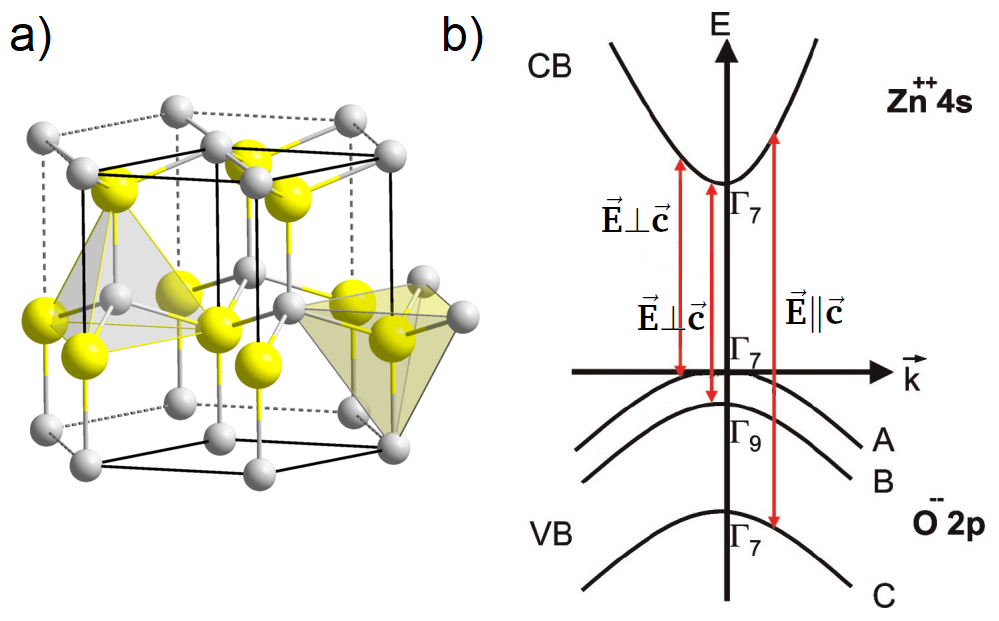
\includegraphics[width=.5\textwidth]{Bilder/Vorbetrachtung/ZnO_Str_BG}
\caption[ZnO Kristall- und Bandstruktur]{Darstellung der a) hexagonalen
Wurzit-Struktur von ZnO mit Zn (gelb) und O (grau) (aus \cite{wurzite}) sowie
der b) Bandstruktur von ZnO um den $\Upgamma$-Punkt mit den verschiedenen
Subbändern (nach \cite{Klingshirn.2010}).} \label{ZnO} \end{figure}
\section{Lumineszenz in II$^b$-VI Halbleitern} \label{ExAn} Dieser Abschnitt
soll eine Übersicht über die wichtigsten exzitonischen Prozesse im Material
geben. Diese sind notwendig, um ein Verständnis für das optische Verhalten von
Halbleitern unter Anregung zu schaffen und ihre Emissionseigenschaften zu
verstehen. \subsection{Exzitonen} Trifft ein Photon mit einer Energie größer
oder gleich der Bandlücke zwischen Valenz- und Leitungsband
$\text{E}_\text{Photon} \geq \text{E}_\text{g}$ auf ein Medium, so kann es
absorbiert werden. Im Falle der Absorption wird ein Elektron aus dem Valenzband
in das Leitungsband angehoben, zurück bleibt eine geladene Fehlstelle
(\textit{Loch}). Um die Energie zu minimieren relaxieren beide Ladungen
materialabhängig im Piko- bis Femtosekundenbereich an die jeweilige Bandkante
(Unterkante des Leitung- bzw. Oberkante des Valenzbandes). Die überschüssige
Energie wird in Form von Gitterschwingungen (\textit{Phononen}) an den
Festkörper abgegeben. Ein solches Elektron-Loch-Paar kann in seiner Beschreibung
als Quasiteilchen betrachtet werden, man spricht von einem \textit{Exziton}.
Dieses Exziton wird durch die Coulombkraft zwischen Elektron und Loch räumlich
zusammengehalten und kann sich im Falle des \textit{freien Exzitons}
(\textit{FX}) im Kristall bewegen. Ähnlich dem Wasserstoffatom kann man auch für
das Exziton einen Bohr'schen Radius $\text{a}_\text{b}$ definieren, der die
Ausdehnung des Exzitons beschreibt: \begin{equation}
a_b=\dfrac{\epsilon\hslash^2}{e^2 \,\mu_{FX}} \qquad\qquad\qquad \text{ mit}
\qquad\qquad\qquad &\mu_{FX}=\frac{(m_e^{\ast} \cdot m_h^{\ast})}{(m_e^{\ast} +
m_h^{\ast})}=\frac{(m_e^{\ast} \cdot m_h^{\ast})}{M}\text{ ,} \end{equation} mit
der Permittivität $\upepsilon$, der Elementarladung e, dem reduzierten Planschen
Wirkungsquantum $\hbar$, der reduzierten Masse des Exzitons $\upmu_\text{FX}$
sowie der effektiven Massen der Elektronen und Löcher m$_\text{e,h}^\ast$.\\ Die
Näherung der effektiven Masse besitzt jedoch nur dann Gültigkeit, wenn die
\mbox{Ausdehnungen} des Exzitons größer als die Elementarzelle des
Materialsystems \mbox{ist \cite{Klingshirn.2007}}. Für ZnO ($\text{a}_\text{b}=
\text{1.8}$ nm \cite{Haranath.2009} gegen $\text{c}= \text{0.52}$ nm) ist dies
erfüllt. Solch schwach \mbox{gebundene} Exzitonen werden auch als
\textit{Mott-Wannier-Exzitonen} bezeichnet. Die Energie des freien Exzitons
beträgt \begin{equation} E_X(\vec{\textit{\textbf{k}}},n_B)= E_g -
R_y\,\frac{\mu_{FX}}{m_0\epsilon^2} \frac{1}{n_B^2}
+\frac{\hslash^2\vec{\textit{\textbf{k}}}^2}{2\,M} \textit{ ,} \label{EX}
\end{equation} mit der Rydbergkonstante $\text{R}_\text{y}$, der Ruhemasse des
Elektrons $\text{m}_\text{0}$, der Hauptquantenzahl des Exzitons
$\text{n}_\text{B}= \text{1, 2, }\ldots $ sowie dem Wellenvektor des Exzitons
$\vec{\textbf{k}}= \vec{\textbf{k$_\text{e}$}}+\vec{\textbf{k$_\text{h}$}}$.
Hierbei wird der zweite Term oft als Exziton-Bindungsenergie bezeichnet, der
dritte Term enthält die kinetische Energie des Exzitons. Die Ausprägung der
Bindungsenergie ist dabei \mbox{maßgeblich} von der Abschirmung durch die
Valenzelektronen des \mbox{Materialsystems} bestimmt. Je lokalisierter diese
sind, desto geringer ist die Abschirmung \cite{Dvorak.2013}. Für ZnO ergeben
sich  Bindungsenergien zu $\text{E}_\text{X,ZnO}=$ 49$\ldots$63 meV
\cite{Mang.1995} bei $\text{n}_\text{B}= \text{1}$ für die drei \mbox{Subbänder}
A, B und C; die Lebensdauer dieser Exzitonen liegt typischerweise im Bereich von
einigen \mbox{hundert Pikosekunden \cite{Zhang.2007}}. Da die Bindungsenergien
höher als die thermische Energie ($\text{k}_\text{b}\text{T} \approx$ 25 meV)
sind, bleiben die Exzitonen des Materialsystems bei \mbox{Raumtemperatur}
stabil. Für thermische Energien größer der Bindungsenergie der Exzitonen
dissoziieren diese.\\ Bei den meisten Halbleiter, so auch in ZnO, kann die
exzitonische Anregung des \mbox{Kristalls} nicht unabhängig vom Lichtfeld
betrachtet werden, da hier eine starke \mbox{Kopplung} \mbox{auftritt}. Ein
Photon bringt eine Polarisation in Form eines Exzitons in den Kristall ein. Das
\mbox{Exziton} rekombiniert und emittiert ein Photon usw. Dieses Quasiteilchen
aus Exziton und Photon wird als \textit{Exziton-Polariton} bezeichnet
\cite{Hopfield.1958}. Die dazugehörige \mbox{Dispersion} ergibt sich aus der
exakten Diagonalisierung des Hamilton-Operators für das gekoppelte System aus
Exziton und Photon und wird in \autoref{PolScat} dargestellt. Hierbei stellt der
obere Ast (engl. \textit{upper polariton branch}, kurz \textit{UPB}) die
Dispersion der longitudinalen exzitonischen Polarisation (die nicht mit dem
\mbox{Lichtfeld} koppelt), der untere Ast (eng. \textit{lower polariton branch},
kurz \textit{LPB}) die \mbox{transversale} \mbox{exzitonische}
\mbox{Polarisation} dar. Oberhalb der Exziton-Resonanz $\text{E}_\text{0}$
erfährt das \mbox{Lichtfeld} die Hintergrunds-Dielektrizitätskonstante
$\upvarepsilon _\text{b}=\upvarepsilon (\infty)$, für Energien darunter die
\mbox{statische} Dielektrizitätskonstante $\upvarepsilon _\text{s}=\upvarepsilon
(\text{0})$. Somit folgt im UPB die Dispersion für \mbox{kleine} \mbox{Werte}
$\vec{\textbf{k}}$ zunächst der exzitonischen Dispersion und nähert sich für
größere Werte der \mbox{photonischen} Dispersion mit der Steigung
$\text{c}/\sqrt{\upvarepsilon _\text{b}}$ an. Im LPB ist es genau
\mbox{andersherum} mit der entsprechenden Steigung der photonischen Dispersion
$\text{c}/\sqrt{\upvarepsilon _\text{s}}$. Polaritonen mit Energien sehr viel
größer $\text{E}_\text{L}$, respektive Energien sehr viel kleiner
$\text{E}_\text{0}$, besitzen folglich einen photonischen Charakter. Anregungen,
wie sie in dieser Arbeit Anwendung finden, geschehen im UPB und können über
akustische oder optische Phononenzweige ins LPB relaxieren
\cite{Klingshirn.2007}.\\ \begin{figure}[htb] \centering
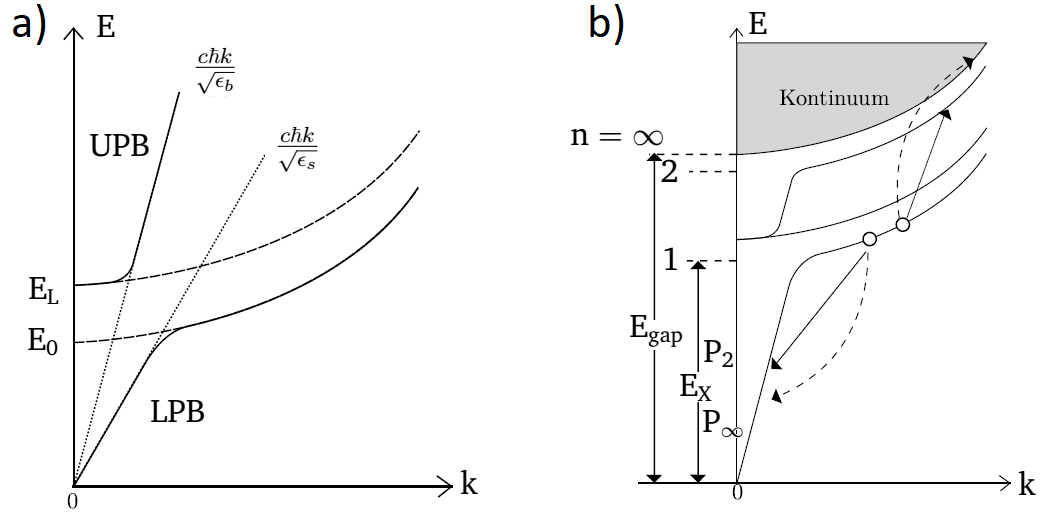
\includegraphics[width=.6\textwidth]{Bilder/Vorbetrachtung/PolScat}
\caption[Polaritonendispersion und inelastische X-X-Streuung]{Schematische
Darstellung der a) Dispersion des Exziton-Polaritons im UPB und LPB. Ebenfalls
eingezeichnet, die Dispersion für Exzitonen (gestrichelt) und Photonen
(gepunktet), sowie der b) inelastischen X-X-Streuung mit
P$_\text{2}$($\longrightarrow$) und P$_\infty$ ($\dashrightarrow$) (beide aus
\cite{Richters.Diss}).} \label{PolScat} \end{figure}
\subsection{Mehr-Exziton-Prozesse} Treffen nun ausreichend viele Photonen
passender Energie pro Zeit und Volumen- element auf ein Material, so erhöht sich
die Zahl der erzeugten Exzitonen und die Wechselwirkung zwischen den einzelnen
Exzitonen kann nicht mehr vernachlässigt \mbox{werden} (s. \autoref{regimes}) –
man spricht vom Bereich mittlerer Anregungsdichte. Es kommt \mbox{vermehrt} zu
elastischen und inelastischen Streuprozessen von Exzitonen an \mbox{Exzitonen}
(\textit{X-X-Streuung}) und an Ladungsträgern \textit{(X-e-} bzw.
\textit{X-h-Streuung}). Es können sich Bi-Exzitonen (\textit{X$_\text{2}$}),
bestehend aus zwei Exzitonen analog zum H$_\text{2}$-Molekül, sowie höhere
Anregungszustände ausbilden \cite{Corfdir.2011}. Die elastische Streuung der
Exzitonen aneinander sorgt hierbei für eine Erweiterung der Resonanz der
Exzitonen, reduziert aber \mbox{gleichsam} ihre Lebensdauer. Bei inelastischer
Streuung wird ein Exziton in einen \mbox{höheren} exzitonischen Zustand gehoben,
während das andere auf den photonischen Ast der Exziton-Polaritondispersion
gestreut wird. Die hierbei entstehende P-Bande wird, je nach erreichtem
Endanregungszustand des in den höheren Zustand gestreuten Exzitons, mit
P$_\text{2}$, P$_\text{3}$, $\ldots$, P$_\infty$ bezeichnet (s.
\autoref{PolScat}). Das so gestreute Exziton relaxiert über Phononen-Streuung
wieder in den Grundzustand zurück \cite{Klingshirn.1975}. Da an diesem
Streuprozess zwei Exzitonen teilnehmen, steigt die Intensität der P-Bande
quadratisch mit der Anregungsdichte an \cite{Priller.2004}. Die strahlende
Rekombination für Biexzitonen erzeugt die sogenannte M-Bande, die für ZnO ca.
12$\ldots$20 meV unterhalb der Energie des freien Exzitons angesiedelt ist.
Hierbei findet ein Zwei-Polariton-Zerfall statt, bei dem zumeist ein
exzitonähnliches und ein photonähnliches Polariton entsteht, die Entstehung
zweier photonähnlicher Polaritonen ist jedoch auch möglich \cite{Hvam.1983}.
\begin{figure}[htb] \centering
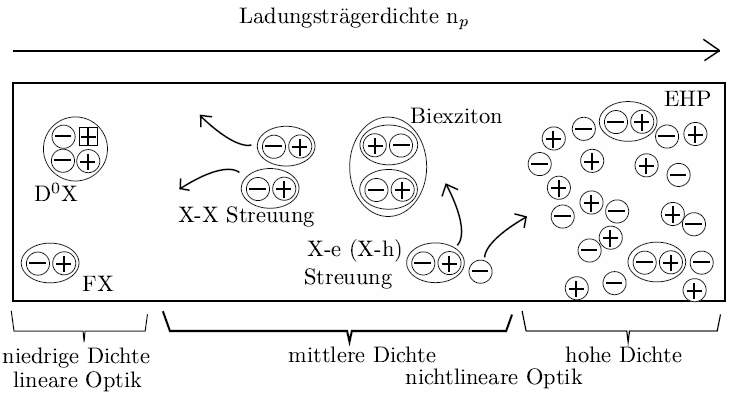
\includegraphics[width=0.7\textwidth]{Bilder/Vorbetrachtung/regimes}
\caption[Übersicht Exzitonen unter hohen Anregungsdichten]{Schematische
Übersicht möglicher Quasiteilchen und deren Wechselwirkung unter verschiedenen
Anregungsdichten (aus \cite{Richters.Diss}).} \label{regimes} \end{figure}
\subsection{Elektron-Loch-Plasma} \label{EHP} Bei noch höheren Anregungsdichten
geht das Gesamtsystem in ein sogenanntes Elektron-Loch-Plasma (engl.
\textit{electron-hole-plasma}, kurz \textit{EHP}) über. Das EHP bezeichnet das
Regime hoher Anregungsdichten und beginnt, sobald der mittlere Abstand der
Exzitonen in etwa ihrem Bohr-Radius a$_\text{B}$ entspricht. Daraus folgt für
die kritische Anregungsdichte n$_\text{p}^\text{c}\approx$
a$_\text{B}^\text{-3}$ \cite{Klingshirn.2007}. Ab dieser Anregungsdichte ist die
Abschirmung der Teilchen untereinander so groß, dass nicht mehr unterschieden
werden kann, welches Elektron an welches Loch gebunden ist. Die Definiertheit
der Exzitonen verschwimmt, sodass nicht mehr von einem Quasipartikel, sondern
vielmehr von einem Plasma gesprochen werden muss (s. \autoref{regimes}). Durch
die starke Abschirmung der Coulombwechselwirkung kommt es zu einer Verminderung
der Bandlückenenergie – man spricht von der sogenannten
\textit{Bandlückenrenormierung}.\begin{figure}[b] \centering
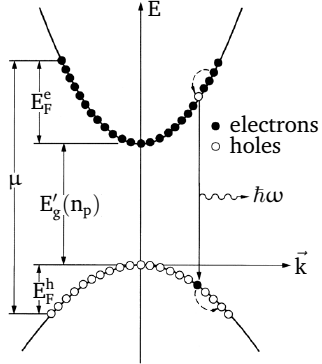
\includegraphics[width=0.3\textwidth]{Bilder/Vorbetrachtung/ehp}
\caption[Besetzung im EHP]{Schematische Darstellung der Besetzung in einem EHP
mit Rekombinationsprozess (nach \cite{Klingshirn.2007}).} \label{Besetzung im
EHP} \end{figure} Diese folgt aus dem Pauli-Prinzip, das den Aufenthalt zweier
Elektronen gleichen Spins im Phasenraum einer Elementarzelle verbietet. Es ist
somit wahrscheinlicher, dass sich in unmittelbarer Nähe des Elektrons ein Loch
aufhält als ein zweites Elektron. Somit überwiegen die anziehenden Coulombkräfte
und die Bandlücke verkleinert sich \cite{Klingshirn.2007}. Im EHP sind sowohl
Valenz- als auch Leitungsband bis zu den Quasiferminiveaus E$_\text{F}^\text{e}$
und E$_\text{F}^\text{h}$ gefüllt (s. \autoref {Besetzung im EHP}). Die
Energiedifferenz beider wird als chemisches Potential $\upmu$ bezeichnet. Bei
steigenden Anregungsdichten laufen die Quasiferminiveaus auseinander, sodass die
spektrale Breite des Spektrums bei strahlender Rekombination \begin{equation}
&\Delta E=\mu -E_g \qquad \qquad \qquad \text{mit }&\mu=E_F^e-E_F^h
\end{equation} zunimmt. \newpage \noindent Da es sich bei ZnO um ein n-leitendes
Material handelt, wird bei zunehmender Anregungsdichte das Donatorniveau immer
weiter aufgefüllt, sodass sich das Ferminiveau nach oben zur
Leitungsbandunterkante verschieben kann. Die daraus resultierende Vergrößerung
der Bandlücke ist als \textit{Burstein-Moss-Effekt} bekannt
\cite{Burstein.1954}. Ein weiterer wichtiger Effekt, der insbesondere bei hohen
Temperaturen und geringen Wärmeleitfähigkeiten zum Tragen kommt, ist die
temperaturbedingte Vergrößerung der Gitterkonstanten, die zu einer Verringerung
der Bandlücke führt, welche quantitativ durch die \textit{Varshni-Formel}
beschrieben wird \cite{Varshni.1967}. \section{Plasmonik}
\subsubsection{Volumenplasmonen} Ein Metall lässt sich im Modell des freien
Elektronengases als Plasma, bestehend aus den positiven Atomrümpfen und den
negativen freien Elektronen, beschreiben. Die schweren Atomrümpfe können
hochfrequenten elektrischen Feldern aufgrund ihrer Trägheit nicht mehr folgen,
wohl aber die um einige Größenordnungen leichteren Elektronen – es kommt zu
einer Ladungstrennung. Diese quantisierte Schwankung der Ladungsträgerdichte im
Festkörper wird gemeinhin als \textit{Plasmon} bezeichnet \cite{Gross.2014}.
Durch innere Streuprozesse der Elektronen an den Gitterrümpfen und anderen
Elektronen wird die Schwingung der Plasmonen gedämpft. Nach dem Drude-Model
ergibt sich die Bewegungsgleichung der Elektronen zu \begin{equation} m_{e}^\ast
\cdot \ddot{\vec{\textbf{x}}} + m_{e}^\ast \cdot \gamma \cdot
\dot{\vec{\textbf{x}}}=-e \cdot \vec{\textbf{E}} \text{ ,} \end{equation} mit
der effektiven Elektronenmasse $\text{m}_\text{e}^\ast$, der Ladung e des
Elektrons, sowie dem Dämpfungskoeffizienten $\upgamma$ der
Elektronenoszillation. Es ergibt sich eine Schwingung mit der Plasmafrequenz
$\upomega_\text{p}$ \cite{Maier.2010}. Plasmonen besitzen entsprechend
näherungsweise die Energie \begin{equation} E=\hbar \cdot \omega_p=\hbar \cdot
\sqrt{\frac{n_e\, e^2}{m_{e}^\ast \cdot \varepsilon}} \text{ ,} \end{equation}
mit der Elektronendichte $\text{n}_\text{e}$ und der Permittivität
$\upvarepsilon$. Die Energie solcher Volumen- plasmonen liegt in der
Größenordnung von etwa 10 meV \cite{Gross.2014}.
\subsubsection{Oberflächenplasmon-Polariton} Oberflächenplasmon-Polaritonen
(engl. \textit{surface plasmon polaritons}, kurz \textit{SPP}) sind Plasmonen,
die sich an der Grenzschicht zwischen dielektrischem und leitendem Material
fortbewegen. Hierbei verweist der Begriff Polariton auf die enge Kopplung einer
sich im dielektrischen Material bewegenden elektromagnetischen Welle an die sich
im leitenden Material bewegenden Ladungen des Elektronengases. Um SSPs
anzuregen, muss der elektrische Feldvektor orthogonal zur Oberfläche
ausgerichtet sein. Die Welle ist somit stark an die Oberfläche gebunden und
evanesziert in beide Materialien \cite{Roeder.Diss}. Verglichen mit den
Volumenplasmonen besitzen sie eine niedrigere Energie, sodass sie optisch
angeregt werden können \cite{Maier.2010}. Mithilfe der Maxwell-Gleichungen und
unter Berücksichtigung der Kontinuitätsbedingung an der Grenzfläche, nämlich
dass die Tangentialkomponente des elektrischen Feldes $\vec{\textbf{E}}$ und die
Normalkomponente der elektrischen Flussdichte $\vec{\textbf{D}}$ stetig sein
müssen, ergibt sich die Dispersionsrelation für SSPs zu \begin{equation}
\beta=\left(\frac{\omega}{c}\right)\cdot \sqrt{\frac{\epsilon_1 \,
\epsilon_2}{\epsilon_1+\epsilon_2}} \text{ ,} \end{equation} mit der
Propagationskonstante $\upbeta$, den Dielektrizitätskonstanten
$\upepsilon_\text{1}$ des Metalls und $\upepsilon_\text{2}$ des Dielektrikums
sowie der Bedingung, dass $\upepsilon_\text{2}<-\upepsilon_\text{1}$. Dies wird
von den meisten Grenzflächen zwischen Metall und Dielektrikum erfüllt. Da fast
alle Metalle über komplexwertige Brechungsindizes
$\upepsilon_\text{1}=\upepsilon'_\text{1}+\upepsilon''_\text{1}$ verfügen, ist
automatisch auch die Propagationskonstante komplex. \section{Lasing in II$^b$-IV
Halbleiternanodrähten} \subsection{Halbleiterlaser} \label{HLLaser} Laser sind
Lichtquellen, die sich durch eine hohe räumliche und zeitliche Kohärenz der
emittierten Strahlung auszeichnen. So haben Laser eine geringe Strahldivergenz
bei einer schmalen Frequenzbreite und einen definierten Polarisationszustand.
Diese Eigen- schaften beruhen auf dem Erzeugungsprozess des Lichtes, der
stimulierten Emission. Hierfür benötigt der Laser drei Bestandteile. Zunächst
wird ein aktives Medium benötigt, das einen strahlenden Übergang bei der
gewünschten Energiez ermöglicht. Diesem Medium muss zweitens durch einen
Pumpprozess genügend Energie zugeführt werden. Für Halbleiterlaser muss so eine
\textit{Besetzungsinversion} (s. \autoref{EHP}) erzeugt werden
\cite{Kneubuhl.2008}. Hierbei sind mehr Elektronen des Valenzbandes in das
Leitungsband angeregt als im Valenzband verbleiben. Dort entsteht ein Überschuss
an Löchern – das System ist also gegenüber dem Grundzustand invertiert
\cite{Kneubuhl.2008}. Damit dies möglich wird, benötigt das aktive Medium
mindestens drei Energieniveaus \cite{Eichhorn.2013}. Um im oberen Laserniveau
eine Überpopulation aufbauen zu können, muss gelten, dass der Übergang des
obersten Niveaus E$_\text{3}$ zum oberen Laserniveau E$_\text{2}$ schneller  als
der Übergang vom oberen Laserniveau in das untere Laserniveau E$_\text{1}$ (hier
der Grundzustand) vonstatten geht \cite{Kneubuhl.2008}. Für ein
Vier-Niveau-System (s. \autoref{Laseruebergang}) kommt, verglichen mit dem
Drei-Niveau-System, ein weiteres Energieniveau $\text{E}_\text{0}$ unter dem
unteren Laserniveau E$_\text{1}$ hinzu. Auch hier gilt, dass der Übergang vom
unteren Laserniveau E$_\text{1}$ zum Grundniveau E$_\text{0}$ sehr schnell
abläuft. Dies hat den Vorteil, das Füllen des unteren Laserniveaus zu verhindern
und so eine Überpopulation im oberen Laserniveau E$_\text{3}$ zu erleichtern.
Das Pumpen kann hierbei optisch oder elektrisch erfolgen. Um stimulierte
Emission zu erhalten, wird als letztes ein optischer Resonator benötigt, der
resonante Moden auswählt und diese in das aktive Medium zurückkoppelt. Die
restlichen Moden werden unterdrückt \cite{Kneubuhl.2008}. \begin{figure}[h]
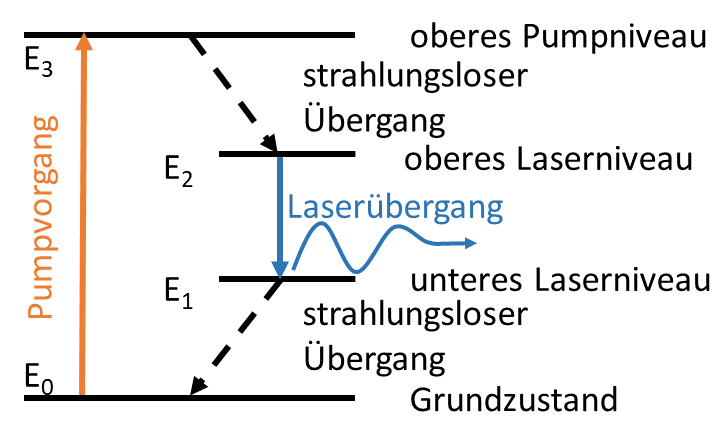
\includegraphics[width=.4\textwidth]{Bilder/Vorbetrachtung/Laseruebergang}
\caption{Laserübergang eines Vier-Niveau-Systems.} \label{Laseruebergang}
\end{figure} \subsection{Lasing in Nanodrähten} Nanodrähte aus ZnO sind aufgrund
ihrer Materialeigenschaften ein aktives Medium und stellen gleichzeitig mit
ihren Wellenleitereigenschaften sowie ihrer durch die hohe Brechzahl bedingten
Reflexion an den Endfacetten einen Resonator dar. Dabei spielen die jeweils
reflektierten Mode und der Durchmesser des Drahtes eine große Rolle, da sich
diese auf den effektiven Brechungsindex auswirken \cite{Maslov.2003}. Im
EHP-Zustand bilden Energiezustände mit hohem $\vec{\textbf{k}}$-Vektor im
Valenz- und Leitungsband, bei einer Absorption von Photonen mit
E$_{\text{Photon}}$ > E$_{\text{g}}$, die Pumpniveaus. Die so entstandenen
Ladungsträger relaxieren durch die in \autoref{ExAn} beschriebenen Streuprozesse
innerhalb von hundert Femtosekunden zu den jeweiligen Bandkanten nahe
$\vec{\textbf{k}}=$ 0, wo der eigentliche strahlende Lasingübergang mit höheren
Lebensdauern stattfindet \cite{Kneubuhl.2008}. Dieses System lässt sich als
Vier-Niveau-System beschreiben \cite{Geburt.Diss}. \subsubsection{Optische
Verstärkung} \label{verst} Bei der Bewegung durch einen Nanodraht verliert eine
elektromagnetische Welle durch Wellenleitung, Absorption, Streuverluste sowie
bei der Reflexion an den Endfacetten an Intensität. Die Schwächung der
Intensität innerhalb des Materials wird durch das Lambert-Beer'sche Gesetz
beschrieben \begin{equation} I(\lambda , L)=I_0 \cdot e^{- \alpha(\lambda)\cdot
L} \text{ ,} \end{equation} mit der Ausgangsintensität I$_{\text{0}}$, dem
wellenlängenabhängigen Absorptionskoeffizienten $\upalpha (\uplambda)$ und der
vom Licht im Material zurückgelegten Strecke L \cite{Eichhorn.2013}. Bei
zunehmenden Anregungsdichten verringert sich der Absorptionskoeffizient
$\upalpha (\uplambda)$ für die betreffenden Wellenlängen der Anregung und kann
im Zustand des EHP sogar negative Werte annehmen; es findet eine Verstärkung
statt, die als verstärkte spontane Emission (engl. \textit{amplified spontaneous
emission}, kurz \textit{ASE}) bekannt ist. Es gilt dann \begin{equation}
&g(\lambda)=-\alpha(\lambda) \qquad \qquad \qquad \text{ und }	&I(\lambda ,
L)=I_0 \cdot e^{g(\lambda)\cdot L} \text{ ,} \end{equation} mit der
Materialverstärkung $\text{g}(\uplambda$), deren spektraler Verlauf in der
\autoref{moden} dargestellt wird. Statt nun mit zunehmender Strecke an
Intensität zu verlieren, steigt die Intensität exponentiell an. Für Photonen mit
Energien $\text{E}_\text{Photon}$ < $\text{E}_\text{g}$ bleibt das Material
transparent, es findet weder Absorption noch Verstärkung statt. Mit Erreichen
der Bandlückenenergie wächst die Verstärkung an. Der Verlauf ist  durch die
Fermifunktionen der Elektronen $\text{f}_\text{e}(\text{E})$ und Löcher
$\text{f}_\text{h}(\text{E})$ sowie der kombinierten Zustandsdichte der Bänder
D$_\text{CDOS}$(E) (engl. \textit{combined desity of states}, kurz
\textit{CDOS}) gegeben \cite{Klingshirn.2007}: \begin{equation} g(E) \sim
(f_e(E) +f_h(E)-1) \cdot D_{CDOS}(E) \text{ .} \end{equation} Am sogenannten
Transparenzpunkt wird die Verstärkung $\text{g}(\text{E}_\text{transp.})=
\text{0}$, er markiert die Energie des höchsten angeregten Zustandes $\upmu$.
Alle Photonen höherer Energie unterliegen einer starken Absorption. Ein
typischer Werte für die maximale Verstärkung von ZnO ist $\text{g} =
\text{7}\cdot \text{10}^\text{3}\text{cm}^\text{-1}$ \cite{Bohnert.1980}. Die
Materialverstärkung $\text{g}(\text{E})$ ist experimentell nicht direkt
zugänglich, sondern nur die \textit{modale Verstärkung}
$\text{g}_\text{mod}(\text{E})$. Die modale Verstärkung beschreibt die
Verstärkung, die das Licht einer bestimmten Mode erfährt, während sie durch das
Material propagiert. Sie ist das Produkt der Materialverstärkung mit einem
Einschlussfaktor $\Upgamma$ \cite{Richters.2012}, der den räumlichen Überlapp
zwischen Lichtwelle und Material beschreibt. \begin{equation} &g_{mod}(E)=\Gamma
\cdot g(E) \qquad \qquad \qquad \text{mit } &\Gamma \in [0,1] \text{ .}
\end{equation} Die modale Verstärkung ist also in der Regel kleiner als die
eigentliche Materialverstärkung. Für größere Durchmesser von Nanodrähten kann
jedoch $ \Upgamma \approx \text{1.2}$ annehmen \cite{Richters.Diss}, da das
Licht in Moden höherer Ordnungen propagieren kann, die nicht parallel zur
Längsachse liegen. Durch diesen ``Zickzackkurs'' legt das Licht einen effektiven
Weg im Nanodraht zurück, der größer als seine eigentliche Länge ist
\cite{Maslov.2004}. Nach der Definition des Einschlussfaktors für planare Wellen
ergibt sich so der höhere Wert.\\ Laseremission kann stattfinden, sobald die
modale Verstärkung im Material die auftretenden Verluste ausgleicht oder
überkompensiert, sprich der Schwellwert $\text{g}_\text{th}$(E) (engl.
\textit{threshold}) \begin{equation} g_{mod}(E)\leq g_{thres.} = \alpha (E)+
\alpha_R(E) +\alpha_W(E) \text{ ,} \end{equation} mit den Absorptions- und
Reflexionsverlusten $\upalpha (\text{E})$, den Wellenleitungsverlusten
$\upalpha_\text{W}(\text{E})$ und den Streuverlusten
$\upalpha_\text{Str}(\text{E})$ erreicht ist, wobei der Verlust durch Reflexion
an den Endfacetten durch \begin{equation} \alpha(E)=\frac{1}{2\,L}\cdot
ln\left(\frac{1}{R_1(E)\cdot R_2(E)}\right) \text{ ,} \end{equation} mit der
Länge L des Resonators und den Reflexivitäten $\text{R}_\text{1,2}$ gegeben ist.
\begin{figure}[b]
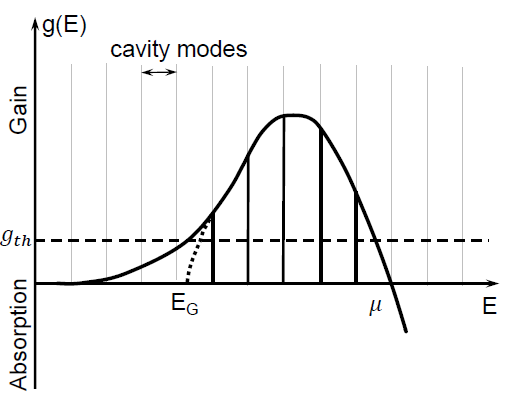
\includegraphics[width=0.35\textwidth]{Bilder/Vorbetrachtung/moden}
\caption[Verstärkungsspektrum eines Halbleiters]{Verstärkungsspektrum eines
Halbleiters zwischen $\text{E}_\text{g}$ und $\upmu$. Schwarz dargestellt sind
die Resonatormoden, deren optische Verstärkung ausreicht, um Lasing oberhalb
einer Schwelle g$_{th}$ zu erreichen (aus \cite{Zapf.Master}).} \label{moden}
\end{figure} \subsubsection{Nanodrähte als Lichtwellenleiter}
Halbleiternanodrähte fungieren, ob ihres hohen Brechungsindex
($\text{n}_\text{NW} \gtrsim 2.5$) verglichen mit ihrer Umgebung
($\text{n}_\text{sur.} \approx 1\ldots 1.5$), als Stufenindexfaser, die die
vollständige Wellenleitung der Lichtwelle innerhalb der Faser gestattet und
somit das Austreten von Licht orthogonal zur Längsachse des Nanodrahtes
unterdrückt \cite{Yao.2009}. Hierbei dient der Nanodraht als eigentlicher Kern,
das umgebende Medium (Vakuum, Luft, Substrat, ...) als Mantel; dieses System
lässt sich als Lichtwellenleiter beschreiben \cite{Pan.2005}. Eine große Rolle
hierbei spielt der Einschlussfaktor $\Upgamma$. Dieser ist generell für
Nanodrähte höher als für konvenionelle, makroskopische Glasfasern
($\Upgamma_\text{NW} \approx$ 1). Nanodrähte, deren Durchmesser einen Wert
$\text{d}_\text{min}\lesssim \uplambda / \text{n}_\text{NW}$ unterschreitet,
schließen das Licht nicht mehr vollständig ein, sodass sich ein Teil der Welle
außerhalb des Drahtes als evaneszente Welle fortsetzt \cite{Voss.2007}. Dieser
Verlauf geht mit starken Verlusten in der Lichtwellenleitung einher. Vor allem
für Nanodrähte, die auf einem Substrat aufgebracht sind, spielt dies eine große
Rolle. Durch den vergleichsweise hohen Brechungsindex $\text{n}_\text{Substr.}
\approx 1.5$ wird der Einschlussfaktor gegenüber dem Substrat stark vermindert,
sodass die Moden zunehmend in das Substrat propagieren. So spielt das Substrat
für größere Durchmesser $\text{d} \geq \text{d}_\text{min}$ eine kleine Rolle,
verglichen mit den Auswirkungen des Substrats auf kleinere Durchmesser der
Nanodrähte. So findet sich unter d $\approx$ 175 nm nur noch die Grundmode, die
für d< 125 nm dann auch verschwindet (s. \autoref{abhd}) \cite{Roeder.Diss}.\\
\begin{figure}[b] \centering
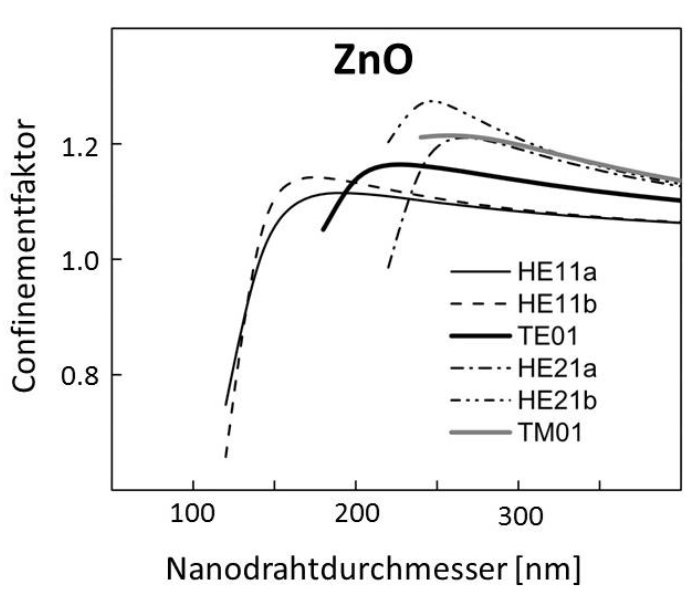
\includegraphics[width=.35\textwidth]{Bilder/Vorbetrachtung/abhd}
\caption[Abhängigkeit des Einschlussfaktors von der Nanodrahtdicke]{Simulierter
Verlauf der Abhängigkeit des Einschlussfaktors von der Dicke des Nano- drahtes
für ZnO auf einem $\text{SiO}_\text{2}$-Substrat (aus \cite{Zimmler.2010}).}
\label{abhd} \end{figure}Man unterscheidet bei der Lichtwellenleitung in
Halbleiternanodrähten zwischen aktivem und passivem Transport. Der aktive
Transport bezieht sich auf Wellenlängen größer als die Bandlücke, die durch
Exziton-Polaritonen weitertransportiert werden und dadurch einer
wegstreckenabhängigen Rotverschiebung im Material unterliegen  \cite{Pan.2005}.
Der passive Transport bezieht sich auf Wellenlängen unterhalb der Bandlücke und
der Urbach-Ausläufer, bei denen – konventionell, wie in Glasfasern – das Licht
entkoppelt von der Exziton-Polariton Wechselwirkung durch den Lichtwellenleiter
propagiert \cite{Klingshirn.2007}.

\subsubsection{Fabry-Pérot-Moden} \label{FPModen} Aufgrund seiner stabförmigen
Geometrie mit den reflektierenden Endfacetten, können Nanodrähte als
\textit{Fabry-Pérot-Resonator} (kurz. \textit{FP}) dienen \cite{Zimmler.2008}.
Durch die Reflexion an den Endfacetten entsteht im Material eine Interferenz der
einlaufenden mit der reflektierten Welle, sodass es zu stehenden Wellen mit
definierten Frequenzen, entsprechend der Resonanzbedingung \begin{equation}
&\lambda_N=\frac{2\,L\cdot n(\lambda)}{N} \qquad\qquad\text{ und}\qquad\qquad
&\Delta \lambda=
\frac{1}{L}\left[\frac{\lambda^2}{2}\left(n(\lambda)-\lambda\cdot\frac{dn(\lambda)}{d\lambda}\right)^{-1}\right]
\text{ ,} \label{ResBed} \end{equation} mit der Wellenlänge
$\uplambda_\text{N}$, der Länge des Resonators L, der Dispersion
$\frac{\text{dn}}{\text{d}\uplambda}$, dem Brechungs- index n($\uplambda)$ sowie
der Modennummer $\text{N} \in \mathbb{N}$, kommt; alle weiteren Frequenzen
inter- ferieren destruktiv. Da jedoch nicht alle Moden eine Verstärkung erfahren
(s. \autoref{moden}) ist N auf die Bereiche
$\text{g}(\text{E})>\text{g}_\text{thres.}$ begrenzt. Der Modenabstand $\Updelta
\uplambda$ ergibt sich \mbox{unter} Berücksichtigung der Dispersion, die
miteinbezogen werden muss, da sich der \mbox{Brechungsindex} von Mode zu Mode
verändert. \subsubsection{Feldverteilung transversaler Moden} Neben den
longitudinalen FP-Lasing-Moden, spielt die Feldverteilung in der Ebene senkrecht
zur Nanodrahtachse eine ebenso herausgehobene Rolle. Sie ist durch die
Transversalmoden gegeben. Diese gliedern sich in transversal-elektrische
($\text{TE}_\text{pl}$), transversal-magnetische ($\text{TM}_\text{pl}$) sowie
ihre hybridisierten Moden ($\text{HE}_\text{mpl}$ bzw. $\text{EH}_\text{pl}$).
In der $\text{TE}_\text{pl}$-Mode existiert nur die elektrische Feldkomponente
senkrecht zur Ausbreitungsrichtung des Lichtes $\vec{\textbf{k}}$, während die
magnetische Feldkomponente in Ausbreitungsrichtung zeigt; bei der
$\text{TM}_\text{pl}$-Mode ist es umgekehrt. Die Hybridmoden enthalten sowohl
elektrische als auch magnetische Komponenten und zeigen in Ausbreitungsrichtung
$\vec{\textbf{k}}$ \cite{Kneubuhl.2008}. Simulierte Feldverteilungen dieser
Moden sind in \autoref{Moden2} abgebildet. Die \mbox{Indizes p, l} bezeichnen
hierbei die Modenzahl bezüglich der Radial- und der Winkel-Komponenten des
Feldes.\begin{figure}[h] \centering
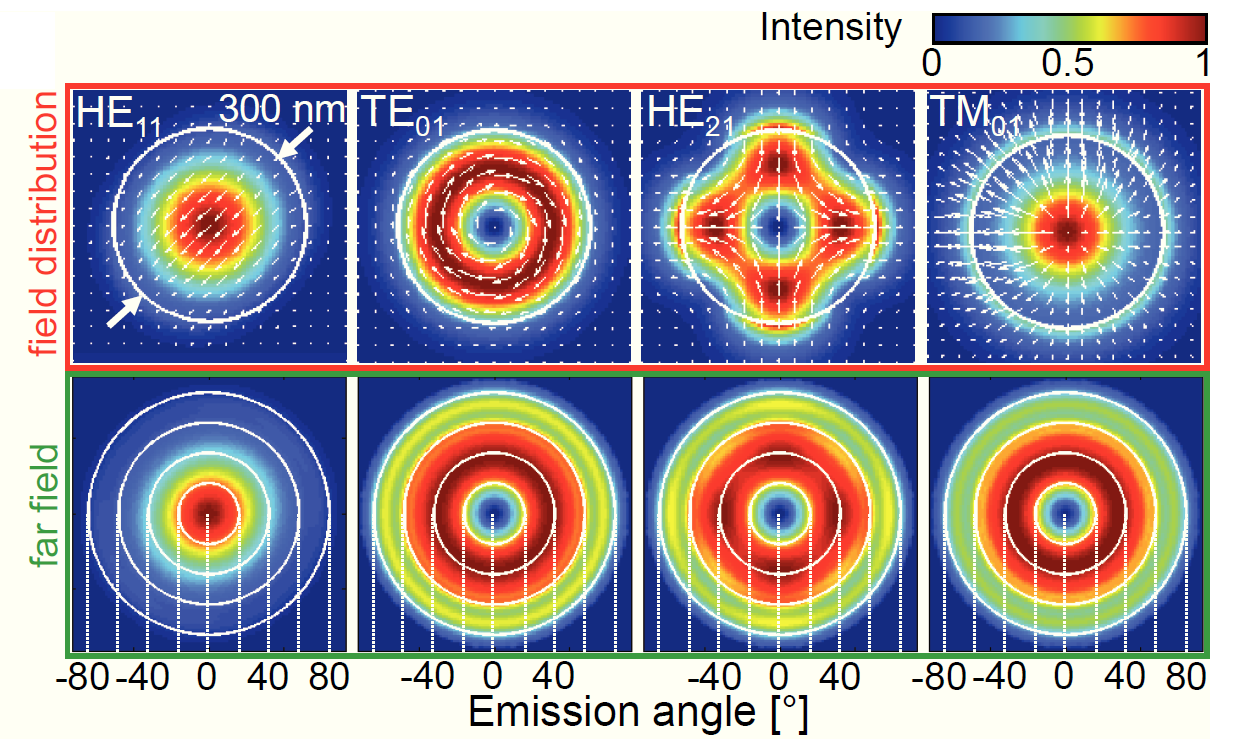
\includegraphics[width=.5\textwidth]{Bilder/Vorbetrachtung/moden2}
\caption[Feldverteilung der Moden eines ZnO-Nanodrahtes]{Simulierte
Feldverteilungen der vier niedrigsten Moden eines zylindrischen ZnO-Nanodrahtes
mit 300 nm Durchmesser ohne Substrat. Oben die Verteilung im Nano- draht, unten
die Emission ins Fernfeld. Jeweils aus Sicht in die Endfacette (aus
\cite{Roeder.Diss}).} \label{Moden2} \end{figure}Für Nanodrähte auf plasmonisch
aktiven Substraten erscheinen zusätzlich zu den photonischen Moden plasmonische
Hybridmoden (engl. \textit{hybrid surface plasmonic mode} kurz \textit{HSP}). Da
der elektrische Feldvektor orthogonal zur Oberfläche eine Grundvoraussetzung für
das Entstehen der SSPs ist, können diese nicht als TE-Mode, sondern
ausschließlich in TM Polarisation vorliegen \cite{Maier.2010}.
\subsubsection{Leistungscharakteristik} Um Lasingverhalten von ASE (s.
\autoref{verst}) zu unterscheiden, muss ein Vergleich mit einem theoretischen
Modell gezogen werden. Da beim Lasing in Nanodrähten verschiedenste Moden
gleichzeitig auftreten und um Verstärkung konkurrieren, können die Moden nicht
einzeln, sondern nur als Gesamtheit betrachtet werden. Etabliert hat sich
hierbei das Multimoden-Laser-Modell nach Casperson (1975) \cite{Casperson.1975}.
Es zeigt analytisch die Abhängigkeit der gesamten emittierten Strahlungsleistung
$\text{x}_\text{t}$ vom Verstärkungs-Verlust-Verhältnis $\text{r}$ pro
Resonatorumlauf. Die auf einen Resonatorspiegel auftreffende Gesamtintensität
aller konkurrierender Lasingmoden ist  durch \begin{equation}
&x_t=\frac{r\,(1+x)^{-1}\,x_0}{\sqrt{1-r\,(1+x)^{-1}}} \qquad \quad \text{mit
}&x_0=x\left[\sqrt{\frac{1+x}{1+x-r}}-1 \right] \end{equation} gegeben. Hierbei
stellt $\text{x}_\text{0}$ ein Maß für den Anteil spontaner Emission in den
Lasingmoden dar. Für jedes r wird der Parameter x aus der impliziten Gleichung
bestimmt. Obige Gleichungen gelten für die Näherung kleiner Frequenzabstände der
longitudinalen Moden gegenüber der Linienbreite des Verstärkungsprofils. An der
Laserschwelle gilt $\text{r}= \text{1}$. Bei einer doppellogarithmischen
Darstellung ergibt sich ein S-förmiger Verlauf. Unterhalb der Lasingschwelle
nimmt die spontane Emission als Funktion der Pumpleistung bzw. des
Verstärkungs-Verlust-Verhältnisses linear zu. Im Bereich um den Laserschwellwert
ist ein starkes nicht-lineares Verhalten der spontanen Emission durch das
Einsetzen der Verstärkung gegeben. Im Lasingbereich ist der Zusammenhang
zwischen gepumpter und emittierter Leistung dann wieder linear.
\begin{figure}[h]
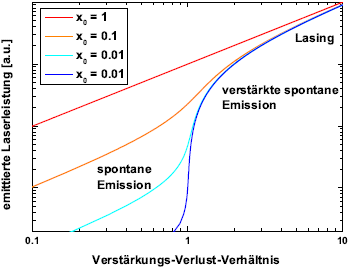
\includegraphics[width=0.4\textwidth]{Bilder/Vorbetrachtung/casperson}
\caption[Lasercharakteristik]{Doppellogarithmische Darstellung der Abhängigkeit
der emittierten Strahlungsleistung als Funktion der Pumpleistung bzw. des
Verstärkungs-Verlust-Verhältnisses (nach \cite{Casperson.1975}).}
\label{casperson} \end{figure} \section{Polarisation und Stokes-Parameter}
\subsection{Polarisationsrichtung von elektromagnetischen Wellen} Neben der
Intensität und der Wellenlänge trägt eine elektromagnetische Welle eine weitere,
nicht direkt messbare Information – die Polarisation. Aus der Lösung der
Maxwell-Gleichungen ergibt sich für den elektrischen Feldanteil im Vakuum
\begin{equation} \vec{\textit{\textbf{E}}}(\vec{\textit{\textbf{r}}},t)=E_0\,
e^{i(\vec{\textit{\textbf{k}}} \cdot \vec{\textit{\textbf{r}}} -\omega t)}
\vec{\textit{\textbf{e}}_{\textit{\textbf{r}}}} \text{ ,} \end{equation} mit der
Ausbreitungsrichtung z folgt daher für die x- und y-Komponente des Feldes
\begin{equation} E_x(\vec{\textit{\textbf{z}}},t)&=E_{0,x} \,
cos(\vec{\textit{\textbf{k}}} \cdot \vec{\textit{\textbf{z}}} - \omega t)\text{
,}\\ E_y(\vec{\textit{\textbf{z}}},t)&=E_{0,y} \, cos(\vec{\textit{\textbf{k}}}
\cdot \vec{\textit{\textbf{z}}} - \omega t + \delta) \text{ ,} \end{equation}
mit der Phasenverschiebung $\updelta$ zwischen den beiden Komponenten. Für
$\updelta= \text{n}\uppi$ ($\text{n} \in \mathbb{Z}$) erfolgt eine lineare
Polarisation in Ausbreitungsrichtung, für $\updelta\neq$ n$\uppi$ ergibt sich
unter Anwendung des Additionstheorems des Kosinus eine Polarisationsellipse
\begin{equation} \left(
\frac{E_x(\vec{\textit{\textbf{z}}},t)}{E_{0,x}}\right)^2 +\left(
\frac{E_y(\vec{\textit{\textbf{z}}},t)}{E_{0,y}} \right)^2-
2\,\frac{E_x(\vec{\textit{\textbf{z}}},t)\,E_y(\vec{\textit{\textbf{z}}},t)}{E_{0,x}\,E_{0,y}}\,cos(\delta)=sin^2(\delta)
\end{equation} einschließlich des Spezialfalles $\updelta = \pm
\frac{\uppi}{\text{2}}$ mit $\text{E}_\text{0,x}=$ E$_\text{0,y}$, in dem sich
zirkular polarisiertes Licht ergibt. Die Hauptachsen der Ellipse müssen dabei
nicht auf denen des Koordinatensystems liegen, sondern können um einen Winkel
$\uppsi$ verschoben sein. Eine aussführliche Beschreibung findet sich bei
Collett (1993) \cite{Collett.1993}. Unpolarisiertes Licht besitzt im Gegensatz
zu polarisiertem, weder ein zeitlich konstantes Phasen- noch
\mbox{Amplitudenverhältnis} und kann somit als Überlagerung vieler linear
polarisierter Wellen aufgefasst werden. \subsection{Stokes-Parameter}
\label{IntroStokesParams} Die Polarisation einer elektromagnetischen Wellen ist
nicht direkt messbar, sie kann aber unter anderem mithilfe eines linearen
Polarisators und eines $\uplambda$/4- Plättchens über die Intensität
rekonstruiert werden (s. \autoref{Mess.Stokes}). Die Intensität ist als
zeitliche Mittellung der quadrierten Feldelemente darstellbar, sodass
\begin{equation} I(\theta)= \underbrace{\left(
E_{0,x}^2+E_{0,y}^2\right)^2}_{=S_0^2}= \underbrace{\left(
E_{0,x}^2-E_{0,y}^2\right)^2}_{=S_1^2} &+ \underbrace{\left(
2\,E_{0,x}\,E_{0,y}\,cos(\delta)\right)^2}_{=S_2^2}+\underbrace{\left(
2\,E_{0,x}\,E_{0,y}\,sin(\delta)\right)^2}_{=S_3^2} \label{StokesGl}
\end{equation} gilt. Die Parameter $\text{S}_{\text{0}\ldots \text{3}}$ werden
nach dem Entwickler dieses Formalismus \textit{Stokes-Parameter} genannt
\cite{Stokes.1851}. S$_\text{0}$ beschreibt hierbei die Gesamtintensität, die
sich aufgliedert: \begin{itemize} \item $\text{S}_\text{1}$, die Differenz
zwischen linear horizontal und vertikal polarisiertem Licht; \item
$\text{S}_\text{2}$, die Differenz zwischen linear $+45^\circ$ und $-45^\circ$
polarisiertem Licht; \item sowie in $\text{S}_\text{3}$, die Differenz aus
rechts- und linkszirkular polarisiertem Licht. \end{itemize} Für Licht mit
Anteilen von polarisiertem und unpolarisiertem Licht geht die obige Gleichung in
eine Ungleichung über: \begin{equation} S_0^2 &\leq S_1^2 + S_2^2 + S_3^2\\
S_0^2 \cdot DOP^2&= S_1^2 + S_2^2 + S_3^2\\ \label{DOPStokes} \Rightarrow
DOP&=\frac{\sqrt{S_1^2+S_2^2+S_3^2}}{S_0} &DOP \in [0,1] \text{ .}
\end{equation} Es wird ein Korrekturfaktor eingefügt, der die Ungleichung zurück
in eine Gleichung überführt. Dieser Faktor DOP wird \textit{Polarisationsgrad}
(engl. \textit{degree of polarization}, kurz \textit{DOP}) genannt. Oftmals
werden die Stokes-Parameter aus praktischen Gründen als Vektor dargestellt.
Unvollständig polarisiertes Licht findet also folgende Darstellung:
\begin{equation} \left( \begin{matrix} S_0 \\ S_1 \\ S_2 \\ S_3 \end{matrix}
\right) = (1-DOP) \left( \begin{matrix} S_0 \\ 0 \\ 0 \\ 0 \end{matrix}
\right)_{UP} + DOP \left( \begin{matrix} S_0 \\ S_1 \\ S_2 \\ S_3 \end{matrix}
\right)_{P} \text{ ,} \end{equation} mit der Aufspaltung in die unpolarisierten
und vollständig polarisierten Anteile \cite{Schaefer.2007}. %Die Drehung
$\Uppsi$ der Polarisationsellipse gegenüber dem Koordinatensystem sowie die
Elliptizität $\upchi$ sind gegeben durch die Verhältnisse der Stokes-Parameter:
%\begin{equation} %\Psi &=\frac{1}{2}arctan\left(\frac{S_2}{S_1}\right)\qquad
\text{mit }\qquad\qquad  0 \leq \Psi \leq \pi \text{ ,}\\ %\chi
&=\frac{1}{2}arcsin\left(\frac{S_3}{S_0}\right)\qquad \text{mit}\qquad\quad
-\frac{\pi}{4} \leq \chi \leq \frac{\pi}{4} \text{ .} %\end{equation}
\section{Magnetismus und Spinpolarisation} Elektronen besitzen, wie alle
Fermionen, einen halbzahligen Spin  s $= \frac{1}{2}$, sowie ein magnetisches
Dipolmoment
$\vec{\boldsymbol{\upmu}}_{\textbf{s}}=\text{g}_\text{e}\upmu_\text{B}\frac{\vec{\textbf{s}}}{\hbar}$.
Es ist also möglich, den Spin mithilfe eines Magnetfeldes auszurichten
\cite{Gross.2014}. Die Ausrichtung des Elektronenspins ist bei der Rekombination
mit einem Loch und der daraus resultierenden Emission eines Photons
mitbestimmend für dessen Polarisationsrichtung (s. \autoref{AusR}). Sie spielt
folglich eine wichtige Rolle im Verständnis der Polarisierbarkeit der Licht- und
Laseremission und soll im Folgenden kurz erläutert werden.
%\subsection{Spin-Bahn-Wechselwirkung} %Im Atom koppelt der Spin der Elektronen
an das Magnetfeld des Kerns. Dieses wiederum hängt maßgeblich vom Bahndrehimpuls
des Elektrons ab, man spricht von der sog. \textit{Spin-Bahn-Kopplung}. Sie
spielt vor allem bei Atomen größerer Masse eine herausragende Rolle, da die
gegenseitige elektrostatische Störung der Elektronen vernachlässigbar wird. Spin
und Bahndrehimpuls der einzelnen Elektronen koppeln zum Gesamtdrehimpulse
$\vec{\textbf{s}}_{\textbf{i}} + \vec{\textbf{l}}_{\textbf{i}}=
\vec{\textbf{j}}_{\textbf{i}}$. Jene koppeln sich zum Gesamtdrehimpuls
$\vec{\textbf{J}}$ des Atoms zusammen $ \vec{\textbf{J}}=\sum_i
\vec{\textbf{j}}_{\textbf{i}}$ . Hierbei sind nur Elektronen unbesetzter Schalen
zu berücksichtigen, da der Gesamtdrehimpuls einer abgeschlossenen Schale sich zu
Null ergibt. Für Atome kleiner Kernladungszahl kann die Spin-Bahn-Wechselwirkung
vernachlässigt werden, hier spielt die spinunabhängige Coulomb-Wechselwirkung
der Elektronen untereinander die entscheidende Rolle. Beschrieben wird dies
durch die LS-Kopplung, bei der sich die Bahndrehimpulse und Spins getrennt
voneinander aufsummieren. Es gilt $ \vec{\textbf{L}}=\sum_i
\vec{\textbf{l}}_{\textbf{i}}$ und $ \vec{\textbf{S}}=\sum_i
\vec{\textbf{s}}_{\textbf{i}}$, beide Gesamtgrößen koppeln dann zum
Gesamtdrehimpuls $ \vec{\textbf{J}}= \vec{\textbf{L}} +  \vec{\textbf{S}}$, der
eine Erhaltungsgröße darstellt. Für die Drehimpulsquantenzahl gilt
$\text{l}=\text{0,1,2 \ldots}<\text{n}$, mit der Hauptquantenzahl n. Oftmals
werden für den Wert dieser Quantenzahl historisch geprägte Buchstaben verwendet,
so wird $\text{l}=\text{0}$ als s-Zustand bezeichnet, $\text{l}=1$ als
p-Zustand, $\text{l}=\text{2}$ als d-Zustand, usw. Eine weitere wichtige
Quantenzahl ist die magnetische Quantenzahl mit $\text{m}_\text{l}=\text{-l, }
\text{-(l-1), }\ldots,\text{(l-1), }\text{l}$, die die zusätzliche Energie der
Elektronen beim Anlegen eines magnetischen Feldes beschreibt.
\subsection{Larmorpräzession und Zeeman-Aufspaltung} \label{Zee} Entsprechend
seines magnetischen Dipolmoments $\vec{\textbf{$\upmu$}}$ erfährt ein Atom oder
Elektron in einem Magnetfeld  $\vec{\textbf{B}}$ ein Drehmoment \begin{equation}
&\vec{\textit{\textbf{M}}}= \vec{\textbf{$\mu$}} \times
\vec{\textit{\textbf{B}}} \qquad \qquad\qquad \text{ und }
&\vec{\textbf{$\mu$}}=g_j \frac{q}{2m} \vec{\textit{\textbf{j}}} \text{ ,}
\end{equation} mit dem Landé-Faktor $\text{g}_\text{j}$, der Ladung q und der
Masse m des Teilchens \cite{Gross.2014}. Dieses Drehmoment bewirkt, dass der
Dipol parallel zum Feld ausgerichtet wird. Als Folge der Drehimpulserhaltung
wird dem Teilchen eine Präzessionsbewegung aufgezwungen. Die Frequenz dieser
Bewegung wird als \textit{Larmor-Frequenz} $\upomega_\text{L}$ bezeichnet und
gibt die zeitliche Änderung des Drehimpulses wieder \begin{equation}
&\frac{d\vec{\textit{\textbf{J}}}}{dt}=
\vec{\textbf{$\omega$}}_{\textit{\textit{\textbf{L}}}} \times
\vec{\textit{\textbf{J}}} \qquad \qquad\qquad \text{ und }
&\vec{\textbf{$\omega$}}_{\textbf{L}}= g_j \frac{q}{2m}
\vec{\textit{\textbf{B}}}. \end{equation} Da es bei Elektronen im
quantenmechanischen Sinne nur zwei Ausrichtung des Spins gibt, kann diese
Präzessionsbewegung nicht als kontinuierliche Drehung verstanden werden, sondern
als Zeit- oder Ensemblemittel der Superposition vieler teilnehmender Elektronen.
Im Fall der LS-Kopplung führt dieser zusätzliche Energieterm zu einer
Aufspaltung der entarteten Energieniveaus nach der Quantenzahl
$\text{m}_\text{j}$ in 2J+1 äquidistante Energieniveaus. Dieser Effekt ist als
\textit{anormaler Zeeman-Effekt} bekannt, der wiederum als Spezialfall
$\text{m}_\text{j}=\text{m}_\text{l}$ bei $\vec{\textbf{S}}=0$ den
\textit{normalen Zeeman-Effekt} beinhaltet \cite{Gross.2014}. Die
Energieaufspaltung beträgt \begin{equation} \Delta E=g_j m_j \frac{q\hbar}{2m}
B. \end{equation} %Bei sehr hohen Magnetfeldern findet eine Entkopplung von Spin
und Bahndrehimpuls statt, die Niveaus verschieben sich weiter und liegen nicht
mehr äquidistant; das Dipolmoment wird zu
$\vec{\textbf{$\upmu$}}=\frac{\text{q}}{\text{2m}}(\text{g}_\text{L}\vec{\textbf{L}}+\text{g}_\text{s}\vec{\textbf{S}})$.
Dieser Effekt ist als \textit{Paschen-Back-Effekt} bekannt \cite{Gross.2014}.
\subsection{Auswahlregeln und Spinpolarisation} \label{AusR} Die Emission oder
Absorption von Photonen folgt strengen Regeln; die Übergangswahrscheinlichkeiten
sind durch \textit{Fermis Goldene Regel} gegeben \cite{Dirac.1927}. Für den
optischen Dipolübergang zur Erzeugung oder Vernichtung eines Exzitons gilt die
Erhaltung des Gesamtdrehimpulses
$\vec{\textbf{J}}=\vec{\textbf{L}}+\vec{\textbf{S}}$. Da das Photon selbst einen
Spin $\vec{\textbf{s}}$ und somit einen Gesamtdrehimpuls von
$|\vec{\textbf{j}}|=|\vec{\textbf{s}}|=\hbar$ trägt, können nur solche Übergange
mit $|\Updelta \vec{\textbf{J}}|=\hbar$ stattfinden. Entsprechend sind auch nur
solche Übergänge der Magnetquantenzahl $\Updelta \text{m}_\text{j}=\text{0,}\pm
\text{1}$ erlaubt. Hierbei gibt $\Updelta\text{m}_\text{j}$ die
Polarisierungsrichtung des Lichtes an: $\Updelta\text{m}_\text{j}=\text{0}$ für
linear polarisiertes ($\pi$), $\Updelta\text{m}_\text{j}=\pm\text{1}$ für
rechts- ($\sigma^{+}$) bzw. linkszirkulär ($\sigma^{-}$) polarisiertes Licht.
Diese Regeln gilt es nun in Relation zu der Bandstruktur zu setzten.\\ Das
Leitungsband in Zinkoxid hat den Drehimpuls
$\text{j}=\text{s}=\frac{\hbar}{\text{2}}$ bei $\text{l}=\text{0}$. Das
Valenzband ($\text{l}=\text{1}$) mit dem Spin $\text{s}=\frac{1}{2}$ ist in drei
Subbänder aufgespalten (s. \autoref{ZnOMat}). Das HH-Band besitzt hierbei einen
Bahndrehimpuls von $\text{j}=\frac{3}{2}$ mit der Magnetquantenzahl
$\text{m}_\text{j}=\frac{3}{2}$, das LH-Band $\text{j}=\frac{3}{2}$ bei
$\text{m}_\text{j}=\frac{1}{2}$ und das SO-Band $\text{j}=\frac{1}{2}$ bei
$\text{m}_\text{j}=\frac{1}{2}$. Diese vier Bänder sind zusätzlich wegen
$\text{s}_\text{z}=\pm\frac{1}{2}$ jeweils doppelt entartet. So ergeben sich die
in \autoref{Ausw} dargestellten möglichen Übergänge mit verschieden
polarisiertem Licht. Um nun eine Spinpolarisation zu generieren, muss einer der
beiden Leitungsbandzustände bevorzugt bevölkert werden. Die Spinpolarisation ist
also eine Abweichung aus der Gleichverteilung und berechnet sich wie folgt
\begin{equation} P=100\%\cdot \frac{\left| N_\uparrow-
N_\downarrow\right|}{N_\uparrow+ N_\downarrow} \text{ ,} \end{equation} mit der
Anzahl N der jeweils Spin-Up und Spin-Down ausgerichteten  Elektronen.
\begin{figure}[h] \centering
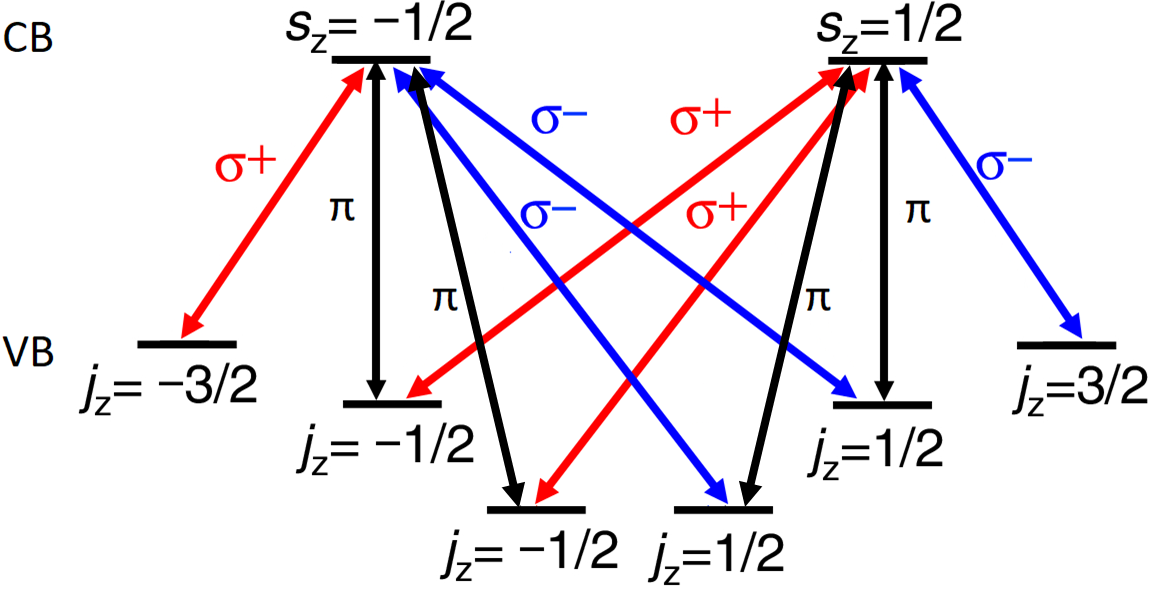
\includegraphics[width=.5\textwidth]{Bilder/Vorbetrachtung/ausw}
\caption[Auswahlregeln]{Mögliche Übergänge von den Valenzbändern in das
Leitungsband unter Berücksichtigung der Auswahlregeln.} \label{Ausw}
\end{figure} \subsection{Spinrelaxation und Spindephasierung} Injiziert man eine
Spinpolarisation in ein angeregtes Elektronensystem, so kann diese nur dann
Einfluss auf die Emissionscharakteristik haben, wenn der Spin länger als die
Rekombinationszeit erhalten bleibt. Es gilt \begin{equation} P=\frac{P_0}{1+
\frac{\tau}{\tau_{SR}}} \text{ ,} \end{equation} mit der Rekombinationszeit der
Elektronen $\uptau$ und deren Spinrelaxationszeit $\uptau_\text{SR}$
\cite{Dyakonov.2008}. Die wichtigsten Mechanismen, die zur Relaxation dieser
Spinpolarisation führen, sollen im Folgenden betrachtet werden.
\subsubsection{Spinrelaxationszeit T$_\text{1}$} Die Spinrelaxationszeit
$\text{T}_\text{1}$ charakterisiert die Rate, in der ein ausgerichtetes Spin-
ensemble wieder das thermische Gleichgewicht mit der Umgebung erreicht. Es gilt:
\begin{equation} M_z(t)=M_{z,eq} -\left[ M_{z,eq}-M_z(0)\right]\cdot e^{t/T_1}
\text{ ,} \end{equation} mit der Magnetisierung in z-Richtung
$\text{M}_\text{z}$, der Magnetisierung im thermischen Gleich- gewicht
M$_\text{z,eq}$ und der verstrichenen Zeit t. T$_\text{1}$ wird auch als
longitudinale Relaxationszeit oder, entsprechend der maßgeblichen
Wechselwirkung, als Spin-Gitter-Relaxation bezeichnet \cite{Zutic.2004}.\\
\subsubsection{Spindekohärenzzeit T$_\text{2}$} Die Spindekohärenzzeit oder
transversale Relaxationszeit T$_\text{2}$ beschreibt die Rate, in der ein mit
Larmorfrequenz um ein Magnetfeld präzedierender Spin seine Phase verliert und
wird maßgeblich von der Spin-Spin-Wechselwirkung verursacht \cite{Fabian.2007}.
Übertragen auf ein Spinensemble findet also eine zunehmende Dephasierung statt.
Es gilt: \begin{equation} M_{xy}(t)=M_{xy}(0)\cdot e^{-t/T_2} \text{ ,}
\end{equation} mit der Magnetisierung in der xy-Ebene $\text{M}_\text{xy}$.
Obwohl beide Relaxationsmechanismen nicht in direkter Verbindung stehen, gilt
für die meisten nichtkubischen Gitter die Näherung \cite{Fabian.2007}
\begin{equation} T_1 = T_2 \text{ .} \end{equation} Je mehr Spins an einem
solchen Spinsystem beteiligt sind, desto mehr Möglichkeiten bestehen, diese
außer Phase zu bringen. Dies wird durch die Spindephasierungszeit
$\text{T}_\text{2}^\ast$ ausgedrückt. Solche zusätzlichen
Dephasierungsmechanismen können beispielsweise durch Variationen des g-Faktors
durch mikroskopische Unregelmäßigkeiten des Kristall- feldes o.ä. entstehen und
verursachen eine inhomogene Linienverbreiterung \cite{Fabian.2007}. Durch diese
Mechanismen verkürzt sich die Zeit, in der ein Ensemble kohärent bleibt.
\subsubsection{Der Elliott-Yafet-Mechanismus} Der Elliott-Yafet-Mechanismus
(kurz \textit{EYM})\cite{Elliott.1954,Yafet.1963} beschreibt das Zusammenspiel
der Spin-Bahn-Wechselwirkung mit einem beliebigen Streuprozess, so z.B. an
anderen Elektronen \cite{Boguslawski.1980}, Phononen oder an Gitterdefekten. Es
kommt im Leitungsband zu einer Mischung von Spin-Up $\ket{\uparrow}$ und
Spin-Down $\ket{\downarrow}$ Zuständen \begin{equation}
\Psi_{\vec{\textbf{k}},n,\uparrow}(\vec{\textbf{r}})=\left(
a_{\vec{\textbf{k}},n}(\vec{\textbf{r}})\ket{\uparrow} +
b_{\vec{\textbf{k}},n}(\vec{\textbf{r}})\ket{\downarrow}\right)\cdot e^{i
\vec{\textbf{k}}\cdot \vec{\textbf{r}}} \text{ ,}\\
\Psi_{\vec{\textbf{k}},n,\downarrow}(\vec{\textbf{r}})=\left(
a_{\vec{\textbf{k}},n}(\vec{\textbf{r}})\ket{\downarrow} +
b_{\vec{\textbf{k}},n}(\vec{\textbf{r}})\ket{\uparrow}\right)\cdot e^{i
\vec{\textbf{k}}\cdot \vec{\textbf{r}}} \text{ ,} \end{equation} mit dem
Bandindex n und $\mid\text{b}_{\vec{\textbf{k}},\text{n}}\mid \ll
\mid\text{a}_{\vec{\textbf{k}},\text{n}}\mid$). Bei solchen Mischzuständen
bleibt der vorhandene Spin bis zu einem Streuereignis konserviert. Erst ein
solches Streuereignis kann den Übergang induzieren – man spricht von einem
\textit{Spinflip}. Die Effektivität des EYM ist also eng mit der
Spinrelaxationszeit $\uptau_\text{SR}$ verknüpft. Es gilt: \begin{equation}
\tau_{SR} \propto \tau_{p} \text{ .} \end{equation} Diese Beziehung ist
charakteristisch für den EYM. %Entsprechend ist der EYM auch stark
Temperaturabhängig zumal bei steigenden Temperaturen vermehrt mit Phononen zu
rechnen ist. So gilt der Zusammenhang $\frac{1}{\uptau} \propto \text{T}$ bei
Temperaturen T größer der Debye-Temperatur $\Uptheta_\text{D}$, für kleinere
Temperaturen gilt $\frac{1}{\uptau} \propto \text{T}^\text{5}$. Der
EY-Mechanismus ist vor \mbox{allem} für Halbleiter mit kleinen Bandlücken und
großen Spin-Bahn-Aufspaltungen des Valenz- bandes effektiv, denn es gilt:
\begin{equation} \frac{1}{\tau_{SR}}=A \cdot
\left(\frac{\Delta_{SO}}{E_g+\Delta_{SO}}\right)^2
\left(\frac{E_k}{E_g}\right)^2  \frac{1}{\tau_p} \text{ ,} \end{equation} mit
einem vom Streuprozess abhängigen numerischen Faktor A, der Bandlücke
E$_\text{g}$, der Spin-Bahn-Aufspaltung des Valenzbandes $\Updelta_\text{SO}$,
sowie der kinetischen Energie des Elektrons vor dem Stoß E$_\text{k}$. Obgleich
ZnO eine vergleichsweise große Bandlücke bei kleiner Aufspaltung des
Valenzbandes besitzt, ist der EYM dominierend für sehr kleine Temperaturen
T$\leq$5 K \cite{Buyanova.2010,Whittaker.1996}. \subsubsection{Der
D'yakonov-Perel'-Mechanismus} \label{DPM} Der D'yakonov-Perel'-Mechanismus (kurz
\textit{DPM}) \cite{Dyakonov.1971} tritt in Materialien ohne Inversions-
symmetrie auf, zu denen u.a. auch ZnO zählt. Hierdurch wird die Entartung der
Spinzustände aufgehoben, es resultiert ein richtungsabhängiges internes
Magnetfeld $\vec{\textbf{B}}(\vec{\textbf{k}}$), in dem der Elektronenspin zu
präzedieren beginnt. Wird nun das Elektron nach einer Zeit $\uptau_\text{p}$
gestreut, verändert sich der $\vec{\textbf{k}}$-Vektor und somit die Richtung
und die Stärke des effektiven Magnetfeldes, um das der Spin des Elektrons
präzediert\cite{Zutic.2004}. Man spricht in diesem Zusammenhang von der
Korrelationszeit $\uptau_\text{c}$, innerhalb derer das fluktuierende Magnetfeld
sich mittelt und als konstant betrachtet werden kann. Es lassen sich hierbei
zwei Fälle unterscheiden: Die Elektonenspins können mindestens einen
vollständigen Präzessionszyklus innerhalb der Korrelationszeit durchlaufen oder
eben nicht. Für den ersten Fall gilt \begin{equation} \tau_c \,\Omega \gg 1
\text{ ,} \end{equation} mit der über $\vec{\textbf{k}}$ gemittelten
Präzessionsfrequenz $\Upomega$. Hierdurch dephasieren die Elektronenspins
aufgrund der Inhomogenitäten des effektiven Magnetfeldes. Die Spin-
relaxationszeit $\uptau_\text{SR}$ ist proportional zur Breite der Verteilung
des effektiven Magnet- feldes und somit zur Korrelationszeit $\uptau_\text{c}$,
es gilt $\uptau_\text{SR} \approx \uptau_\text{c}$.\\ %Der Prozess ist
reversibel \cite{Hu.2002}. Für den zweiten Fall gilt \begin{equation} \tau_c
\,\Omega \ll 1 \text{ .} \end{equation} Dieser als \textit{``motional
narrowing''} bekannte Fall wird vom DPM beschrieben und \mbox{ähnelt} viel mehr
der Präzession in einem inhomogenen Magnetfeld. Die Spinrelaxationszeit lässt
sich mit dem Modell eines \textit{Random-Walk} abschätzen. Zwischen zwei
Streuprozessen präzediert der Spin um den Winkel $\upvarphi=\uptau_\text{c} \,
\Upomega$. Nach einer Zeit t ist der Erwartungswert des quadrierten Drehwinkels
$\Braket{\Updelta\upvarphi^\text{2}}$ proportional zur Anzahl der
Random-Walk-Schritte $\text{t}/\uptau_\text{c}$ multipliziert mit der
quadrierten Schrittweite $(\Upomega\, \uptau_\text{c})^\text{2}$
\begin{equation} \Braket{\Delta\upvarphi^2} \sim \Omega^2\,\tau_c t \,\text{ .}
\end{equation} Die Spinrelaxationszeit $\uptau_\text{SR}$ ist hierbei über die
Bedingung $\Braket{\Updelta\upvarphi^\text{2}} \sim \text{1}$ bei
$\text{t}=\uptau_\text{SR}$ gegeben, sodass \begin{equation}
\frac{1}{\uptau_{SR}} \sim \Omega^2\, \tau_c \end{equation} folgt. Dieser
Zusammenhang ist charakteristisch für den DPM. Die Spinrelaxationszeit steigt
also mit der Häufigkeit der Streuprozesse. Generell gilt also $\uptau_\text{SR}
\gg \uptau_\text{c}$.  Anschaulich können die Spins dem Wechsel des Magnetfeldes
nicht mehr folgen und behalten somit ihre ursprüngliche Orientierung.\\ Der DPM
ist für Halbleiter ohne Inversionssymmetrie für Temperaturen $\text{T}>\text{5}$
K der dominierende Prozess. Er dominiert in undotierten und n-dotierten
Systemen, die die Bedingung des \textit{``motional narrowing''} erfüllen
\cite{Zutic.2004}. Zudem wurde von Whittaker et al. (1996) \cite{Whittaker.1996}
theoretisch gezeigt, dass \textit{``motional narrowing''} in qualitativ
hochwertigen Halbleiter-Mikrokavitäten zu erwarten ist. \subsubsection{Einfluss
eines externen Magnetfeldes auf den D'yakonov-Perel'-Mechanismus}
\label{DPM_Mag} Legt man nun zusätzlich ein homogenes externes Magnetfeld an,
präzidieren die Spins mit der Larmor-Frequenz
$\upomega_\text{L}=\text{g}_\text{j}\frac{\text{q}}{\text{2m}}\vec{\textbf{B}}$
um das Magnetfeld $\vec{\textbf{B}}$. Für den Fall eines homogenen internen
Feldes, bleibt der Spinvektor konstant – Relaxation kann nur über die
Inhomogenitäten erfolgen. Liegen die Inhomogenitäten des inneren Magnetfeldes in
Richtung des externen Magnetfeldes, so spielt das Vorhandensein des externen
Feldes keine Rolle für die transversale Spinrelaxationszeit $\text{T}_\text{2}$,
da sich das Feld durch Rotation nicht ändert. Es bleibt bei der
charakteristischen Zeit $\text{T}_\text{2} \approx \uptau_\text{SR}$.\\ Für die
senkrecht zum externen Magnetfeld stehenden Fluktuationen ergibt sich ein
anderes Bild; in diesem Fall rotiert der Spinvektor mit der Larmor-Frequenz
durch die Inhomogenitäten. Sie beeinflussen die Spinrelaxation in Richtung des
externen Feldes und somit die longitudinale Spinrelaxationszeit
$\text{T}_\text{1}$, die damit von der Stärke des externen Magnetfeldes abhängig
wird.\\ Für $\uptau_\text{c}\upomega_\text{L} \ll \text{1}$ spielt diese
Präzessionsbewegung eine untergeordnete Rolle, da sich das Feld schon zuvor in
der Zeit $\uptau_\text{c}$ geändert hat. Für den Fall das $\uptau_\text{c}
\upomega_\text{L} \gg \text{1}$ rotiert der Spinvektor hingegen so schnell, dass
sich die Inhomogenitäten des inneren Feldes effektiv herausmitteln. Die
longitudinale Spinrelaxationszeit $\text{T}_\text{1}$ steigt mit:
\begin{equation} \frac{1}{T_1}=\frac{1}{\tau_{SR}}\frac{1}{1+(\omega_L
\tau_{c})^2}=\frac{\Omega^2 \tau_c}{1+(\omega_L \tau_{c})^2} \text{ .}
\end{equation} Quantenmechanisch gesprochen kann der Spin nur longitudinal
relaxieren, wenn sich die Spinprojektion auf $\vec{\textbf{B}}$  umdreht. Dies
erfordert die Energie $\text{E}=\hbar\upomega_\text{L}$. Da das fluktuierende
interne Feld eine Energie von $\text{E}=\hbar/\uptau_\text{c}$ bereitstellen
kann, wird der Prozess bei $\upomega_{L}\gg\text{1}/\uptau_\text{c}$ oder
äquivalent $\upomega_{L}\uptau_\text{c}\gg\text{1}$ ineffektiv, der Spinvektor
bleibt über lange Zeiträume unverändert. Durch Anlegen eines ausreichend starken
externen Magnetfeldes ändert sich also der proportionale Zusammenhang zwischen
der longitudinalen Spinrelaxationszeit $T_\text{1}$ und der Korrelationszeit
$\uptau_\text{c}$ zu einem antiproportionalen \cite{Dyakonov.2008}.\\ Mit
steigendem Magnetfeld wird also die Relaxationszeit T$_\text{1}$ vermindert und
sättigt bei einem Wert ab, der durch den EYM vorgegeben ist \cite{Bronold.2002}.
\subsubsection{Der Hanle-Effekt} \label{Hanle} Der Hanle-Effekt
\cite{Hanle.1924} beschreibt die Depolarisation von Spins in \mbox{einem}
\mbox{Materialsystem}, das einem externen transversalen Magnetfeld ausgesetzt
ist. Hierbei liegt der \mbox{Ursprung} dieses Effektes in der Präzession der
Elektronenspins um das \mbox{Magnetfeld}. Dieses führt unter kontinuierlicher
Anregung zu einer Verminderung der durchschnittlichen Projektion der
Elektronenspins auf die Richtung der Observablen, die den
\mbox{Polarisationsgrad} der Lumineszenz bestimmt. Die Bewegung des gemittelten
Spinvektors ist gegeben durch \begin{equation} \frac{d\vec{\textbf{S}}}{dt}=
\vec{\textbf{$\omega_L$}}\times
\vec{\textbf{S}}-\frac{\vec{\textbf{S}}}{\tau_{SR}}-
\frac{\vec{\textbf{S}}-\vec{\textbf{$S_0$}}}{\tau} \text{ ,} \end{equation} mit
der Spinpräzession im Magnetfeld als erstem Term, der Spinrelaxation im zweiten
Term mit der Spinerzeugung der optischen Anregung
($\vec{\textbf{$\text{S}_\text{0}$}}$/$\uptau$) sowie der Rekombination der
spinpolarisierten Elektronen ($-\vec{\textbf{$\text{S}$}}$/$\uptau$) im dritten
Term. Die Projektion auf die z-Achse ergibt sich somit zu \begin{equation}
&S_z(B)= \frac{S_0}{1+(\omega_L\tau^\ast)^2} \qquad \qquad \qquad \text{mit}
&\frac{1}{\tau^\ast}=\frac{1}{\tau}+\frac{1}{\tau_{SR}} \text{ ,} \end{equation}
mit der effektiven Polarisationszeit $\uptau^\ast$, die die Breite der
Depolarisationskurve angibt. Die Spinprojektion nimmt also als Funktion des
transversalen Magnetfeldes ab \cite{Dyakonov.2008}. \chapter{Experimentelle
Methodik} \section{Synthese und Präparation der Nanodrähte}
\subsection{Nanodrahtsynthese via VLS-Mechanismus} Die im Rahmen dieser
Masterthesis untersuchten ZnO-Nanodrähte wurden im Hoch- temperaturofen (kurz
\textit{HTJ}) nach dem von Wagner und Ellis (1964) beschriebenen
Vapor-Liquid-Solid Mechanismus (kurz \textit{VLS}) \cite{Wagner.1964} gewachsen.
Auf ein phosphordotiertes n-Typ Si-[100] Substrat wurde eine 10nm dicke
Goldschicht aufgesputtert. Das Quellmaterial war ein Pulver bestehend aus
Zinkoxid (ZnO) und Kohlenstoff (C) zu gleichen Stoffmengenanteilen. Letzterer
dient zur Reduktion der Sublimationstemperatur. Sowohl Substrat als auch
Quellmaterial wurden in kleine Keramikschiffchen gegeben und in einem Rohr im
Innern des HTJ positioniert. Dabei wurde das Schiffchen mit dem Quellmaterial an
der Position der höchsten Temperatur $\text{T}_\text{max}$ platziert, das des
Substrates an einer Position geringerer Temperatur (s. \autoref{htj}). Der
Wachstumsdruck p wurde eingestellt und Argongas (Ar) eingeleitet, das während
der Erhitzung und letztendlich der Verdampfung des Quellmaterials einen
Volumenfluss $\text{Q}_\text{Ar}$ bereitstellte, der das verdampfte
Quellmaterial eine Wachstumszeit $\text{t}_\text{w}$ lang zum Substrat trans-
portierte. Diese Parameter sind übersichtlich in \autoref{Params}
zusammengestellt. ZnO adsorbiert vorzugsweise an der Oberfläche der bei dieser
Temperatur flüssigen Goldtropfen. Mit fortschreitender Adsorption erreicht das
Wachstumsmaterial in den Goldtropfen eine Übersättigung, in deren Folge es an
der Grenzfläche zum Substrat auskristallisiert, da die hier aufzuwendende
Oberflächenenergie am geringsten ist. Es entstehen ein- kristalline Nanodrähte
mit einer Länge von ca. 10 - 50 $\upmu$m und einem Durchmesser von ca. 100 - 500
nm. Zeitgleich hierzu findet ein als Vapor-Solid (kurz \textit{VS}) benannter
Ablagerungsprozess statt. Dieser sorgt dafür, dass sich das Wachstumsmaterial
auch an die Seitenflächen der Nanodrähte anlagert; es können daher segelförmige
Auswüchse an den Nanodrähten entstehen. Dennoch wird der Durchmesser der Drähte
weiterhin primär vom Durchmesser der Goldtropfen bestimmt, da der VS-Prozess
verglichen mit dem VLS-Prozess um Größenordnungen langsamer verläuft
\cite{Geburt.Diss}. \begin{table} \begin{tabular}{llll} Wachstumsdruck p &
Temperatur $\text{T}_\text{max}$ & Wachstumszeit $\text{t}_\text{w}$ &
Ar-Volumenfluss $\text{q}_\text{Ar}$ \\ 100 mbar & 1350 $^{\circ}$C & 60 min &
50 sccm \\ \end{tabular} \caption[VLS-Wachstumsparameter]{Übersicht über die
verwendeten Wachstumsparameter der VLS-Drahtsynthese.} \label{Params}
\end{table} \begin{figure} \centering
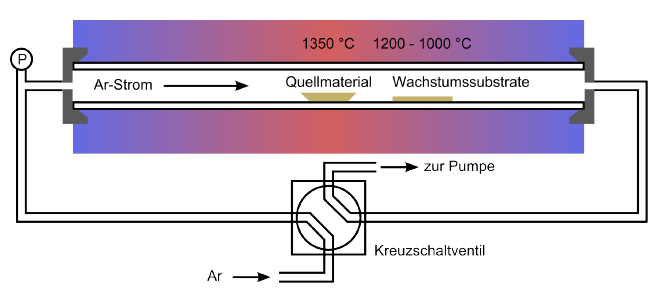
\includegraphics[width=.75\textwidth]{Bilder/Methodik/htj}
\caption[Schematischer Aufbau des HTJ-Ofens]{Schematischer Aufbau des HTJ-Ofens
mit den Temperaturzonen und der Positionierung des Quellmaterials sowie der
Wachstumssubtrate (aus \cite{Thielmann.Dipl}).} \label{htj} \end{figure}
\subsection{Imprint} Auf den via VLS-Mechanismus gewachsenen Nanodrahtproben
stehen die Drähte sehr eng beieinander. Um einzelne Drähte anzuregen, muss die
Anzahl der Nanodrähte pro Flächeneinheit reduziert werden. Dies wird durch das
sogenannte \textit{Imprinten} der Probe erreicht. Hierbei wird die
Wachstumsprobe mit geringem Druck über ein sauberes Substrat gezogen. Es brechen
einige Drähte ab und bleiben durch Van-der-Waals-Kräfte an dem Substrat
haften.\\ Diese ``Imprints'' wurden im Rahmen dieser Masterthesis sowohl mit
Siliziumdioxid (SiO$_\text{2}$), als auch mit
Magnesiumoxid-Cobalt-Siliziumdioxid ( MgO/Co/SiO$_\text{2}$) als Substrat
angefertigt. Das MgO/Co/SiO$_\text{2}$-Substrat gliedert sich in mehrere
übereinanderliegende Schichten auf. Unter einer 3 nm dünne Schicht MgO liegt
eine  magnetisierbare, 20 nm dicke Cobaltschicht (Co) auf einem
SiO$_2$-Bulk-Material. %Die Idee hinter dem Aufbau dieses Substrats zielt auf
den Proximity-Effekt ab, denn durch den geringen Abstand vom Nanodraht zur
magnetisierbaren Cobaltschicht kommt es zur spontanen Spinkohärenz
\cite{Epstein.2002}. Die MgO-Schicht wirkt als sowohl als Oxidationsschutz für
die dünne Cobaltschicht und reduziert die plasmonischen Verluste, sodass sich
schon bei geringeren Anregungsdichten Lasing einstellen kann.\\ Das
MgO/Co/SiO$_\text{2}$-Substrat wurde am Forschungszentrum Jülich hergestellt und
von der Arbeitsgruppe um Prof. Jia Grace Lu von der University of Southern
California mit einer Vierpunktmessung auf den anisotropen magnetoresistiven
Effekt untersucht. \subsection{Magnetisierung der Probe} \label{MagProb} Um die
Weiß'schen Bezirke der Cobaltschicht auszurichten, wird ein Magnetfeld von ca.
10 mT benötigt. Dieser Wert ergibt sich aus der Magnetowiderstandsmessung (s.
\autoref{magres}) des Substrates.\begin{figure}[b] \centering
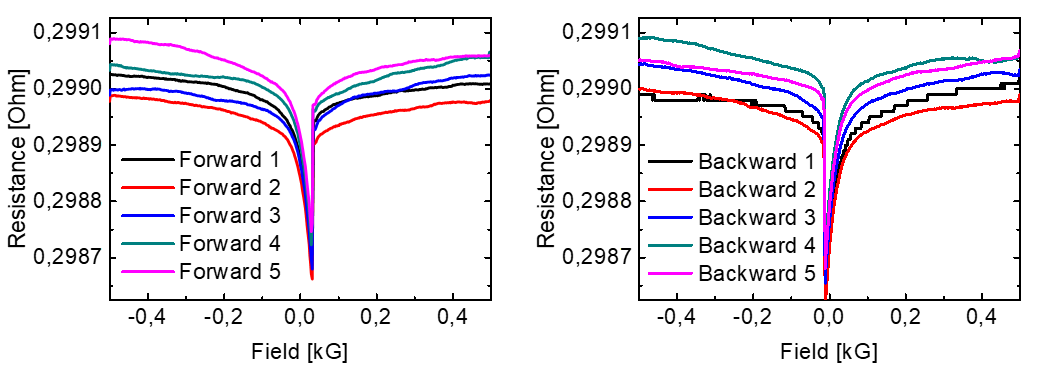
\includegraphics[width=.85\textwidth]{Bilder/Methodik/magnres}
\caption[Magnetowiderstandsmessung des
MgO/Co/SiO$_\text{2}$-Substrates]{Magnetowiderstandsmessung des
MgO/Co/SiO$_\text{2}$-Substrates (\cite{Mag}). Es wird ersichtlich, dass ein
Magnetfeld von 10mT (0.1 kG) bereits ausreichen, um die Weiß'schen Bezirke
auszurichten.} \label{magres} \end{figure}Hierbei wurde der elektrische
Widerstand des Substrates in Abhängigkeit von einem externen Magnetfeld
gemessen, das im Verlauf der Messung umgepolt wurde. Es zeigt sich bei der
Koerzitivfeldstärke eine kleine Abnahme des Widerstandes, die aus der Unordnung
der Spins resultiert, gefolgt von einer steilen Flanke, die in einen
Sättingungsbereich mündet. Hier werden zunehmend alle Spins der Weiß'schen
Bezirke ausgerichtet, das Substrat ist maximal magnetisiert. Genau diese
Sättigung der Magnetisierung soll erreicht werden. Um sicherzugehen, dass dieser
Bereich definitiv erreicht wird, wurde das Magnetfeld um den Faktor fünf höher
dimensioniert, als theoretisch nötig wäre. Um gleichzeitig eine möglichst hohe
Vergleichbarkeit der Magnetfeldstärke über das Substrat zu gewährleisten, soll
eine Spulenanordnung nach Helmholtz verwendet werden. Die Besonderheit an dieser
Spulenanordnung ist, dass beide Spulen mit dem gleichen Radius R im Abstand
ihres Radius platziert werden. Zwischen den Spulen entsteht ein homogenes
Magnetfeld, dass sich zu \begin{equation} B=\mu_0 \cdot \frac{8}{\sqrt{128}}
\cdot \frac{I \cdot N}{R} \end{equation} berechnet \cite{Demtroeder.2009}. \\
Das im Rahmen dieser Masterthesis angefertigte Spulenpaar erlaubt \textit{in
situ} die Spulenanordnung 90$^\circ$ um die ortsfeste Probe im PL-Aufbau in die
horizontale (Feldlinien orthogonal zur Nanodrahtachse) bzw. vertikale Position
(Feldlinien parallel zur Nanodrahtachse) zu drehen und somit eine Veränderung
der Emissionscharakteristik zu bestimmen (s. \autoref{AufbauPL}). Da sich eine
Anordnung der Spulen streng nach dem Helmholtz-Aufbau nicht in den
Versuchsaufbau inkludieren lässt, wurde ein höherer mittlerer Spulenabstand als
der Radius der Spulen gewählt. Die Maße der Spule sind in \autoref{HSpule}
zusammengefasst. Die resultierenden Inhomogenitäten des Magnetfeldes mit
entsprechenden Feldstärken wurden mittels der Finiten-Elemente-Methode (FEM)
simuliert (s. \autoref{Sim} a)) und variierten um 5\% über die Ausdehnung der 2
cm breiten Probe (s. \autoref{Sim} b) und c)). Referenzmessungen mithilfe eines
Magnetometers (Koshava 5 K102304) bei 10.5 A, mit einem Digitalmultimeter
(Peaktech 3325) in der Mitte der Helmholtzspule gemessen, ergaben eine maximale
Magnetfeldstärke von (49 $\pm$ 2) mT und sind somit einen guten Anhaltspunkt für
die Übereinstimmung des simulierten mit dem gemessenen Magnetfeld. Die
Spulenanordnung wurde so in den optischen Aufbau eingesetzt, dass das Substrat
mittig zwischen den Spulen lag. \begin{table}[h] \centering \begin{small}
\begin{tabular}{lllll} Windungszahl N & mittl. Radius r & mittl. Spulenabstand d
& Widerstand R & Stromstärke I\\ 325 & 45 mm & 65 mm & 2.1 $\Upomega$ & 10.5 A\\
\end{tabular} \end{small} \caption[Dimensionierung der Helmholtzspule]{Übersicht
über die Parameter der Helmholtzspule.} \label{HSpule} \end{table}
\begin{figure}[h] \centering
\includegraphics[width=1\textwidth]{Bilder/Methodik/Sim_mag_komplett}
\caption[Simulation des Magnetfeldes der Spule]{a) Simulation der Feldstärke B
des Magnetfeldes nach der FEM mit Profilen in der b) x-Achse bzw. c) z-Achse der
Helmholtzspule.} \label{Sim} \end{figure} \section{Charakterisierung der Proben}
\subsection{Mikro-Photolumineszenz Aufbau} Um die Lasercharakteristik der
Nanodrähte zu untersuchen, wurde im Rahmen dieser Masterthesis auf den
Mikro-Photolumineszenzaufbau (kurz \textit{$\upmu$-PL}) zurückgegriffen (s.
\autoref{AufbauPL}). Als Anregungslichtquelle wurde ein Neodym-dotierter
Yttrium-Aluminium-Granat (kurz \textit{Nd:YAG})-Laser der Firma Innolas (Model:
SL Compact DPSS100) verwendet. Hierbei handelt es sich um einen Festkörperlaser,
der bei einer Grundwellenlänge von \mbox{1064 nm} Licht emittiert. Diese
Wellenlänge kann mithilfe nichtlinearer optischer Kristalle gedrittelt werden,
sodass für die Experimente Anregungslicht der Wellenlänge \mbox{$\uplambda=$
355 nm} zur Verfügung stand. Dabei war der Nd:YAG-Laserstrahl mit nominell 7 ns
bei einer Repetitionsrate von 100 Hz gepulst. Mithilfe  einer Kombination aus
$\uplambda$/2-Platte und Brewsterpolarisator wurde horizontal polarisiertes
Licht erzeugt. Anschließend wurde das Laserlicht durch ein
\textit{Pellin-Broca-Prisma} gelenkt. Dieses Dispersionsprisma trennt weitere im
Strahl vorhandene Spektrallinien von der Anregungsfrequenz. Der Strahl kann
durch Neutraldichtefilter stufenlos um dreizehn Größenordnungen abgeschwächt
werden und trifft danach auf einen Strahlteiler, der einen Teil des Strahls
zwecks Intensitätsmessung auf eine Si-Diode der Firma Thorlabs (Modell: S130VC)
abzweigt. Über einen weiteren Strahlteiler wird Weißlicht eingekoppelt. Beide
Strahlen werden in das Objektiv (NUV Plan Apo, 50x, infinity corrected, NA=0.42)
der Firma OptoSigma geleitet. Eine weitere Linse (f$=$300mm) im alleinigen
Strahlengang des Lasers sorgt für dessen Aufweitung, sodass der Laserspot einen
anderen Fokuspunkt als das Weißlicht hat, die Nanostrukturen also gleichzeitig
im Weißlichtfokus beobachtbar bleiben, während der Laserspot genügend ausgedehnt
bleibt, um den kompletten Draht auszuleuchten. Die zu untersuchende Probe wurde
mithilfe eines XYZ-Piezo-Probentischs in den Weißlichtfokus gefahren und ein
passender Draht gesucht. Über einen klappbaren Spiegel kann das Bild auf eine
TV-Kamera gelenkt werden, die Apparatur fungiert als Lumineszenz-Mikroskop und
ermöglicht die Orientierung auf der Probenoberfläche. Für die Messung wurde das
Licht durch eine weitere Linse (f=150mm) auf einen Gittermonochromator der Firma
Princeton Instruments (Model: Acton SP2500i) abgebildet. Für winkelaufgelöste
Messungen kann zusätzlich die Linse L2 in den Strahlengang geklappt werden.
Mithilfe eines Langpassfilters wird das Photolumineszenzlicht von der
Anregungsstrahlung getrennt.  Zur Auswahl stehen drei verschiedene Gitter mit
verschiedenen Gitterliniendichten von 150, 400 und 1200 mm$^{-1}$, die eine
spektrale Übersicht, bzw. ein hochaufgelöstes Spektrum bieten. Die Messungen
dieser Master- thesis wurden jedoch ausschließlich mit dem dritten Gitter
angefertigt, da der Bereich der FP-Moden möglichst genau dargestellt werden
soll. Desweiteren kann die Spaltbreite des Eingansschlitzes variiert werden, um
mehr Licht in den Monochromator zu lasten der Auflösung zu lassen. Die Detektion
der Photonen erfolgt schlussendlich in einem stickstoffgekühlten CCD-Detektor
mit 1024 x 256 Bildpunkten und 26 $\upmu$m Breite, der einen Wellenlängenbereich
von typischerweise 200-1000 nm detektieren kann.\\ Die Messgeometrie folgt dem
klassischen Auflichtmikroskopaufbau in der Anregung und Detektion in einer Achse
liegen, der Nanodraht wird in Draufsicht (engl. \textit{top view}) betrachtet.
\\ Da im Rahmen dieser Transferleistung der $\upmu$-PL Aufbau deutlich
abgeändert wurde, befindet sich im Anhang eine Justageanleitung (s.
\autoref{Justage}). \begin{figure}[h] \centering
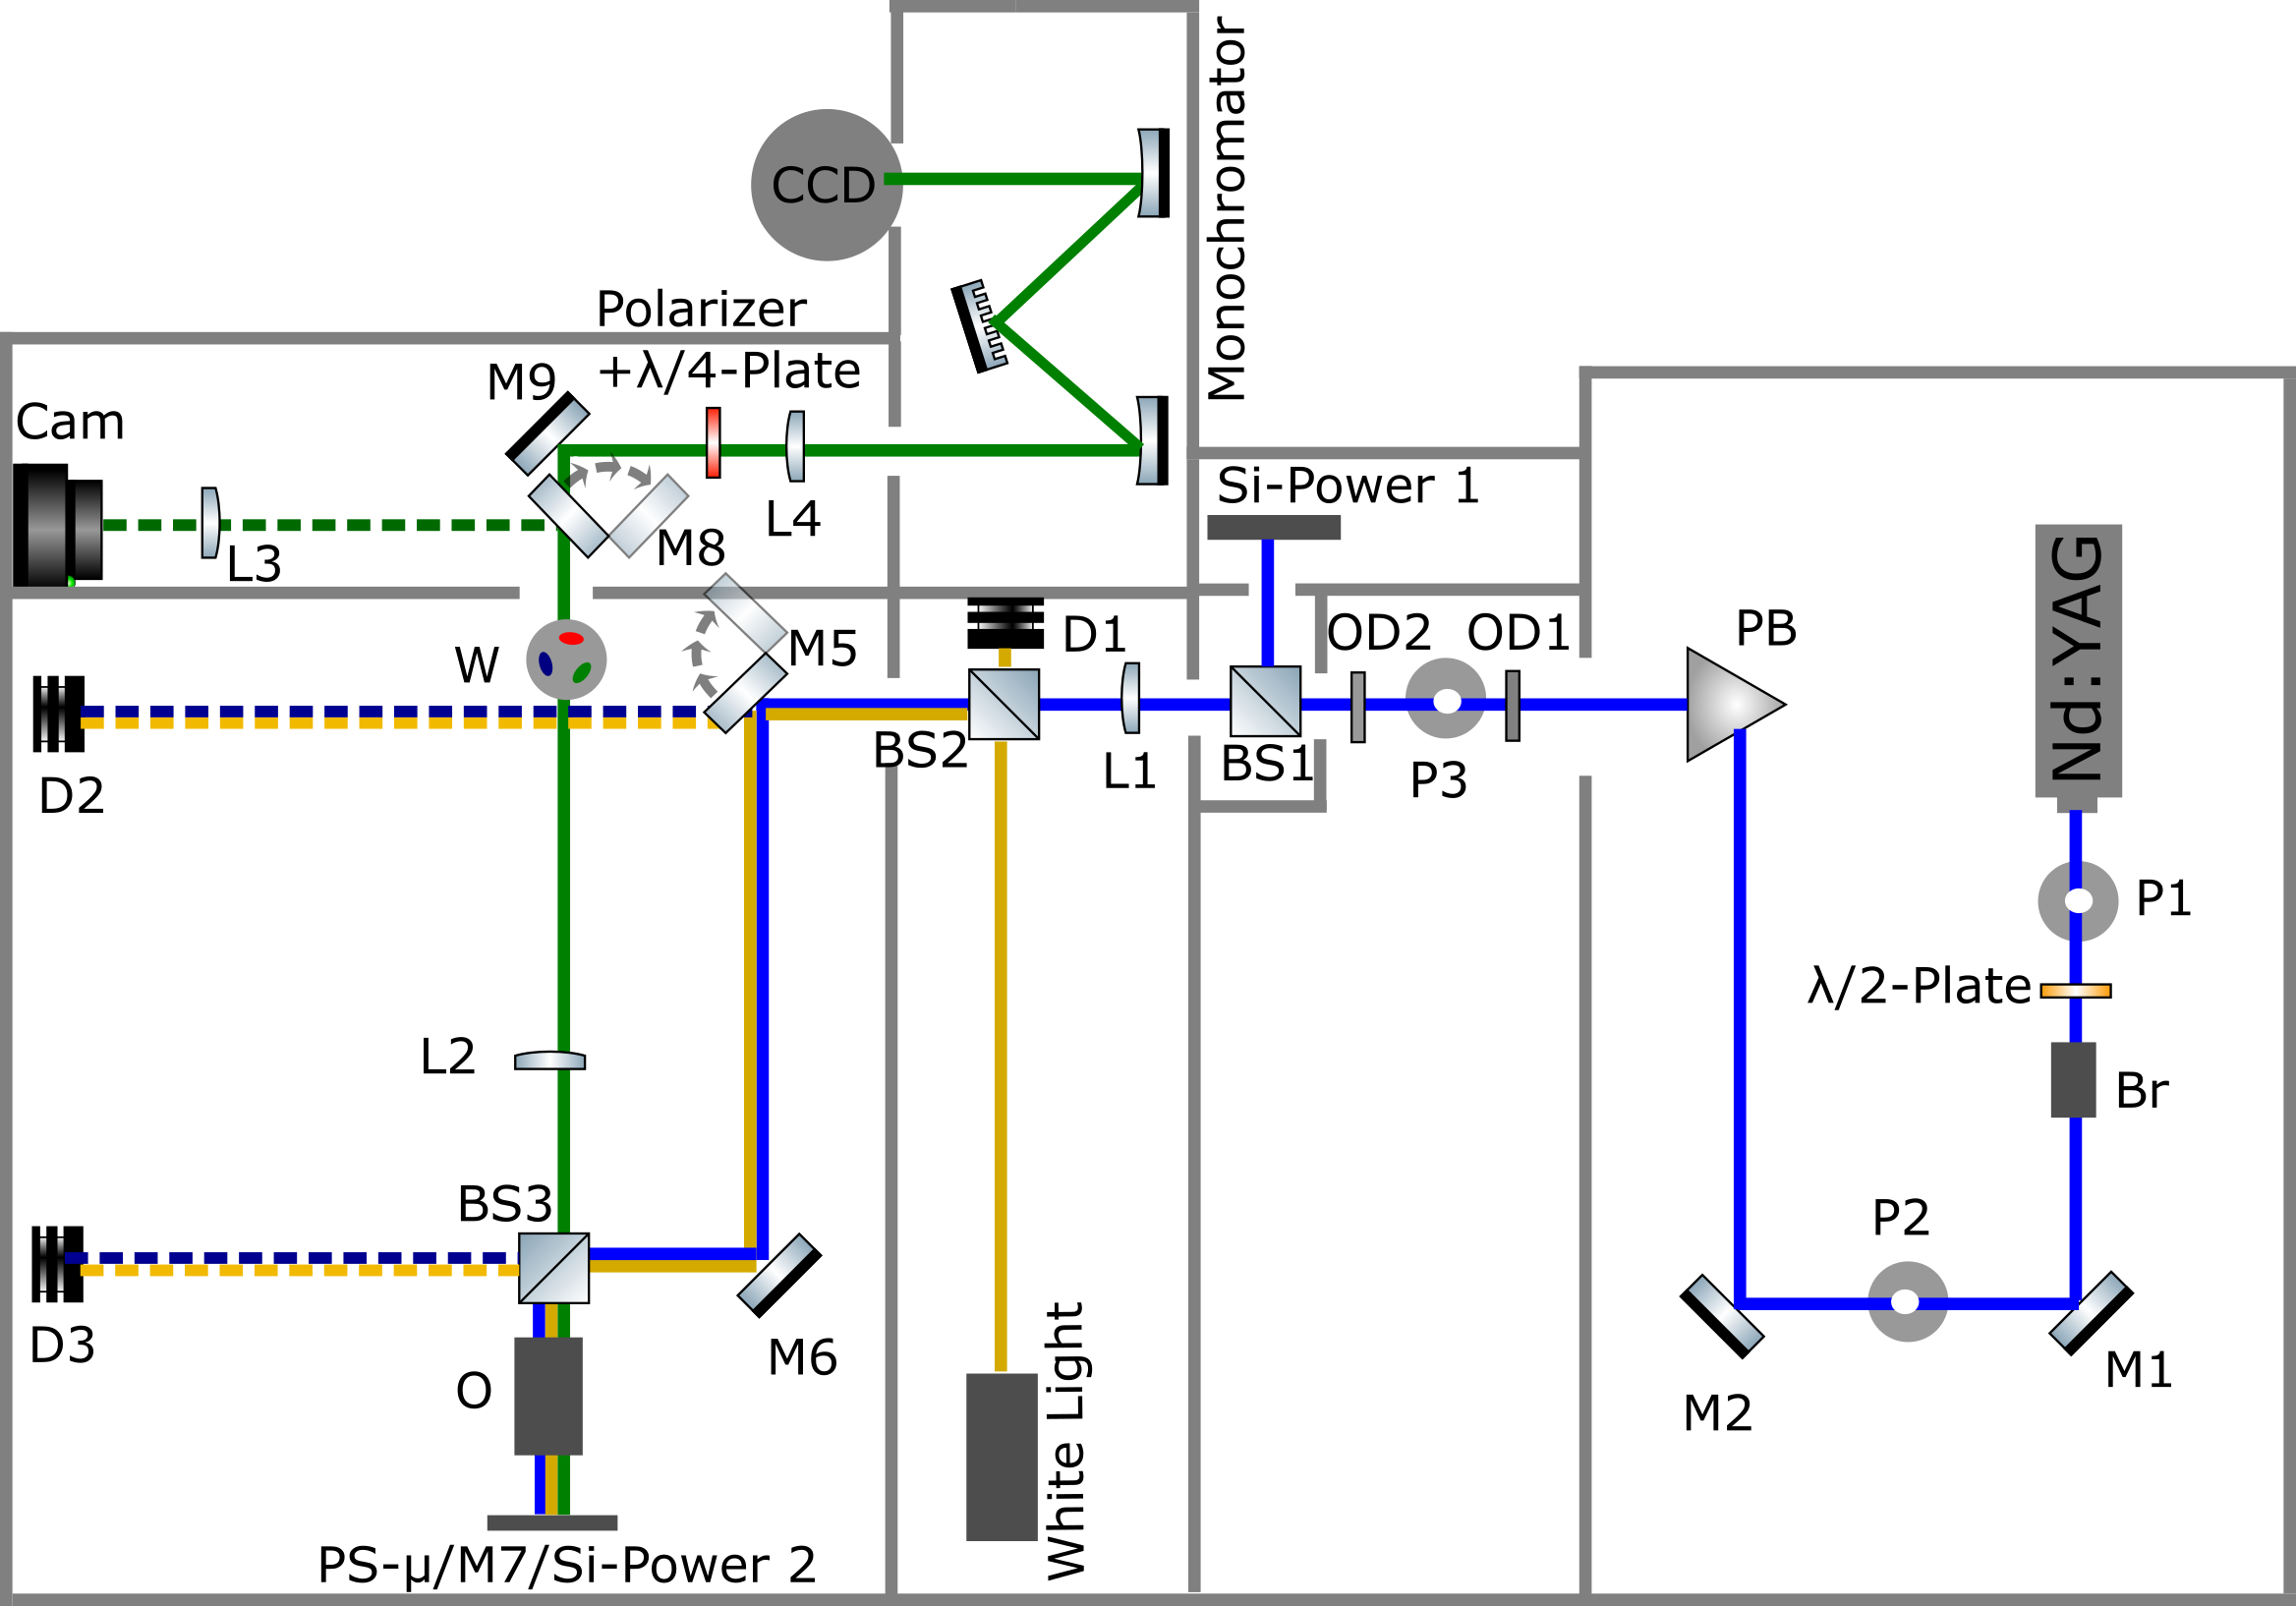
\includegraphics[width=1\textwidth]{Bilder/methodik/opt_aufb} \caption[Aufbau
$\upmu$-PL]{Aufbau der $\upmu$-PL, erstellt mit Incscape und ComponentLibrary
\cite{lib}. Mit den Komponenten: Spiegel (MX), Lochblende (PX), Linse (LX),
Strahlteiler (BSX), Beamdump (DX), Filterrad (W), Objektiv (O),
Pellin-Broca-Prisma (PB), Neutraldichtefilter (ODX), Brewster Polarisator (BR),
$\upmu$-PL Probentisch (PS-$\upmu$).} \label{AufbauPL} \end{figure}
\subsubsection{Kalibrierung der Leistungsdichte} Zunächst wurde der Laserstrahl
mithilfe der Lochblenden und Linsen so eingestellt, dass er eine möglichst
homogene Ausleuchtung des Nanodrahtes aufwies. Eine Intensitätskarte des
Laserspot findet sich in \autoref{laserspot} a). Während der gesamten Messungen
dieser Masterthesis wurde der Spot nicht verändert, um die Ergebnisse
vergleichbar zu halten.\\ Die Anregungsintensität am Probenort während der
Messung wurde an der Position ``Si-Power 1'' \textit{in situ} gemessen und
mithilfe einer Kalibrierungssmessung angepasst. Hierzu wurden im Vorhinein
Laserintensitäten an Position ``Si-Power 1'' und ``Si-Power 2'' in Bezug
gesetzt. Der Zusammenhang wurde für einzelne Leistungsbereiche näherungsweise
als linear angenommen, so ergeben sich für die Einzelbereiche die Zusammenhänge
als \begin{equation} I(\text{Si-Power 2})=  a \cdot I(\text{Si-Power 1})  + b
\text{ .} \end{equation} Diese Anpassungsbereiche sind dargestellt in
\autoref{laserspot} b). Vor jeder Leistungsmessung wurde mit der Si-Diode an
beiden Positionen jeweils neu genullt, der Messbereich der Diode wurde manuell
und noch weit vor Ausreizung des Messbereiches umgestellt. Es zeigte sich, dass
die voreingestellten Wechsel der Messbereiche die dargestellte Intensität als zu
niedrig angaben. Es kommt dabei zu teils drastischen Absättigungseffekten, die
durch den manuellen Wechsel umgangen werden konnten. Weitere Anmerkungen hierzu
befinden sich im Anhang im \autoref{Leistmess}. \\ Die Größe des Laserspots
wurde vor jeder Messung an den Nanodrähten mit Hilfe der TV-Kamera aufgezeichnet
und anhand eines Referenzbildes eines genormten Markersubstrates im
Weißlichtfokus bestimmt. Aus der Laserleistung am Probenort sowie der Größe des
Laserspots ergibt sich die Leistungsdichte. Der Nanodraht wurde in den
Folgemessungen mithilfe des Probentisches in den Weißlichtfokus gerückt, es
wurde darauf geachtet, dass der Draht parallel zum Monochromatoreingang
ausgerichtet, mittig im Laserspot lag und vollständig ausgeleuchtet war. Im
Folgenden wurde die parallele Ausrichtung des Nanodrahtes zur Öffnung des
Monochromatoreingangs als ``\textit{vertikal}'' bezeichnet. Die Ausrichtung
parallel zum optischen Tisch und orthogonal zur Monochromatoröffnung wird als
``\textit{horizontal}'' bezeichnet. \begin{figure} \centering
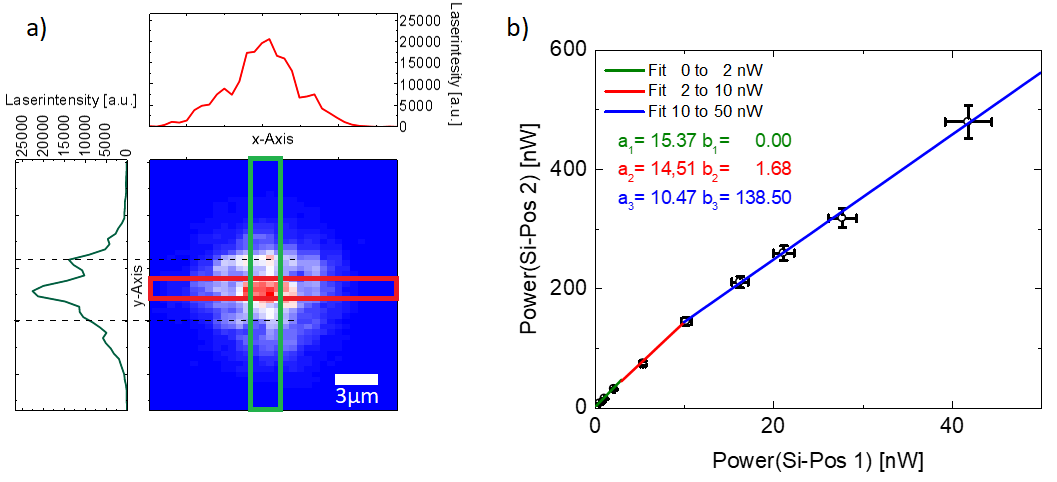
\includegraphics[width=1\textwidth]{Bilder/Methodik/spotsize}
\caption{Darstellung der a) Intensitätskarte des Laserspots mit Linienprofilen
über 5 Pixel in x-Richtung (parallel zur Lage des Nanodrahtes) und y-Richtung
mit Hilfe der CCD-Kamera. Gestrichelt dargestellt wird die Positionierung der
Nanodrähte in y-Richtung. Darstellung b) zeigt die Kalibrierungsmessung der
Laserleistung an ``Si-Pos 1'' und ``Si-Pos 2''.} \label{laserspot} \end{figure}
\subsubsection{Erstellung der Lasingkurven} Um sicher festzustellen, dass sich
der Nanodraht im Lasingbereich befindet, wurde nach dem Casperson
Multimoden-Laser-Model (s. \autoref{casperson}) eine Anpassung erstellt, aus dem
sich die Schwellwert-Leistungsdichte ergab. Hierzu wurde vor den PL-Messungen am
Nanodraht zunächst der Strahlungshintergrund auf der CCD-Kamera ermittelt und in
den Folgemessungen abgezogen. Die Leistungsdichte wurde schrittweise erhöht und
die zugehörige Modenspektra aufgezeichnet. Die Integrationszeiten der CCD-Kamera
betrugen 1-10 Sekunden bei einer Spaltbreite des Monochromatoreingangs von 150
$\upmu$m. Für die Anpassung nach Casperson wurden diese Spektren zeitlich
normiert und der Bereich der FP-Moden spektral integriert. Die so gewonnenen
Intensitäten wurden über der Anregungsdichte aufgetragen. Mithilfe eines
Matlabskriptes wurden der x$_\text{0}$-Parameter und die Lasingschwelle
angenähert.\\ Bei allen Messungen wurde darauf geachtet, den Draht nicht in den
Degradationsbereich kommen zu lassen \cite{Zapf.2017}. Für weiterfolgende
Messungen wurde die Anregungsintensität so gewählt, dass sie zwischen dem
1.2-fachen bis doppelten der Laserschwelle lag; somit wurde sichergestellt, dass
der Draht sich im Lasingbereich befand und wenig degradierte.
\subsubsection{Fourier Optik} \begin{figure}[h] \centering
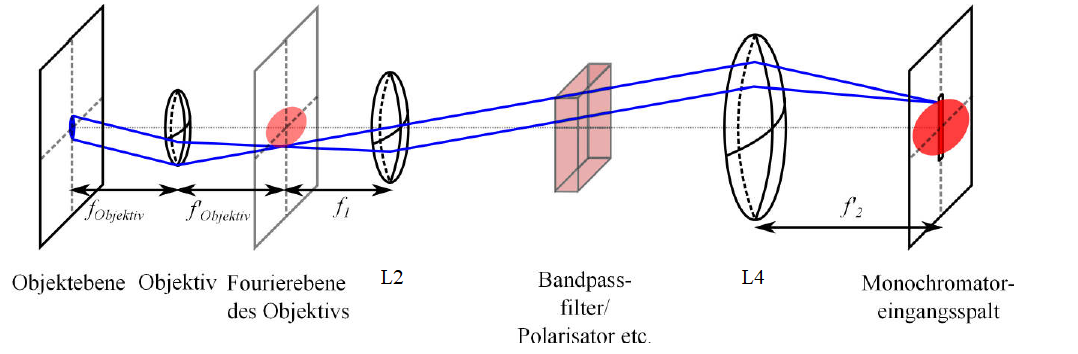
\includegraphics[width=1\textwidth]{Bilder/Methodik/fourier}
\caption[Impulsraumabbildung]{Strahlengang durch den Fourieraufbau. Die
Fourierebene des Objektivs wird auf den Monochromatoreingang abgebildet und
erlaubt so die Emission des Nanodrahtes winkelabhängig aufzulösen (aus
\cite{Master.Michalsky}).} \label{FLense} \end{figure} \noindent Um die
Richtungsabhängigkeit der Emissionsintensität des Nanodrahtes aufzuschlüsseln
wurde eine weitere Linse L2 im Abstand ihrer Brennweite hinter dem Objektiv
platziert. Sie bildet somit die rückseitige Fourierebene des Objektivs (engl.
\textit{back focal plane}) mit Linse L4 auf den Eingangsspalt des Monochromators
ab. Da die Strahlen aus einem Punkt der Fourierebene parallel zwischen beiden
Linsen verlaufen (s. \autoref{FLense}) hat der Abstand beider Linsen zueinander
keinen Einfluss auf die Skalierung des Bildes, wohl aber das Verhältnis ihrer
beiden Brennweiten. Dieser Faktor berechnet sich zu
$\text{M}_\text{F}=\frac{\text{f}_\text{2}}{\text{f}_\text{1}}$. Für eine
größtmögliche Ausleuchtung des CCD-Detektors unter den räumlichen Gegebenheiten
wurden die Linsen zu f$_\text{1}=\text{125}$ mm und f$_\text{2}=\text{150}$ mm
gewählt, somit ergibt sich die Vergrößerung zu $\text{M}_\text{F}=\text{1.2}$.
Zwischen den Linsen L2 und L4 wurden alle optischen Bauteile für die
Stokes-Messung untergebracht. Der maximal darstellbare Raumwinkel ist gegeben
durch die numerische Apertur NA des Objektivs und die optische Dichte
n($\uplambda$) des Mediums zwischen Objektiv und Sample und berechnet sich zu
\cite{Riediger.Master} \begin{equation}
\uptheta_{max}=arcsin\left(n(\uplambda)\cdot NA\right) \text{ .} \end{equation}
Mit dem in dieser Masterthesis verwendeten Objektiv (NA$=$0.43) kann somit ein
maxi- maler Raumwinkel von $\uptheta_\text{max} \approx \text{25}^\circ$
aufgelöst werden. Da die Fourierabbildung mit einer Abbildungslinse auf die CCD
abgebildet wird, ist eine Entzerrung des Bildes bzw. Korrektur der Intensitäten
(vgl. \cite{Roeder.Diss,Riediger.Master}) nicht notwendig. Eine ausführliche
Herleitung der Korrenkturfaktoren, die ohne Abbildungslinse notwendig wären,
befindet sich im Anhang (s. \autoref{correct}). \\ Die vorgenommenen Messungen
gliedern sich in zwei Teilbereiche. Zunächst wurde das Fourierbild direkt, also
in nullter Beugungsordnung des Monochromators, betrachtet. Die Belichtungsdauer
betrug 100 Sekunden, der Eingangsspalt des Monochromators war 6 mm weit
geöffnet, um das komplette Bild aufzunehmen. Auch hier wurde zunächst eine
Messung des Strahlungshintergrundes vorgenommen, der im Folgenden von den
Messbildern abgezogen wurde.\\ Diese Messart bietet den Vorteil sich eine
Übersicht über den maximal auflösbaren Bereich der Raumwinkel zu verschafften.
Jedoch liegen die Charakteristiken der einzelnen FP-Moden und der spontanen
Emission in diesem Bild übereinander und können nicht getrennt voneinander
betrachtet werden, da in diesem Modus nicht spektral aufgelöst wird.\\ Um eine
spektrale Auflösung zu erreichen, können auch Messungen in erster
Beugungsordnung des Monochromators durchgeführt werden und somit die Moden
einzeln betrachtet werden. Für die spektrale Aufspaltung ist jedoch eine kleine
Öffnung des Monochromatoreingangs nötig, da sonst die spektrale Auflösung zu
gering ist, die Moden effektiv zu trennen. Für diese Art der Messung wurde der
Monochromatoreingang auf 500 $\upmu$m geöffnet – bei dieser Öffnungsweite waren
die Moden gerade vollständig voneinander getrennt. Da nun aber nur ein kleines
Segment der Raumwinkel dargestellt wird, wurde das Fourierbild über den
Monochromatoreingang variiert, sodass für verschiedene Kreissegmente eine
spektrale Aufspaltung möglich war. Auch hier betrug die Belichtungsdauer 100
Sekunden.\\ Es war ein Blazegitter im Monochromator verbaut, somit sind die
reflektierten Intensitäten in erster Beugungsordnung gegenüber der nullten
Beugungsordnung erhöht. Eine Beschreibung der Einmessung der Fourieroptik ist im
Anhang detailliert beschrieben (s. \autoref{fourier}). \subsubsection{Messung
der Stokes-Parameter} \label{Mess.Stokes} \begin{figure}[h]
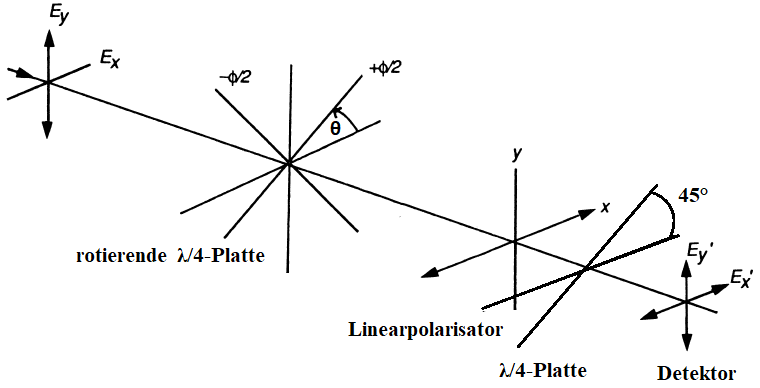
\includegraphics[width=.8\textwidth]{Bilder/Methodik/stokesaufbau}
\caption{Aufbau nach der Methode der rotierenden $\uplambda$/4-Platte mit der
Transmissionsachse des Polarisators. Die schnelle optischen Achse der
$\uplambda$/4-Platte in horizontaler Ausrichtung und einer Drehung der
$\uplambda$/4-Platte entgegen des Uhrzeigersinnes aus Sicht des Detektors (nach
\cite{Goldstein.2003}).} \end{figure} \noindent Die Messung der Stokes-Parameter
erfolgt nach der Methode der rotierenden $\uplambda$/4-Platte. Hierzu wird in
den Aufbau ein Linearpolarisator (Thorlabs Model: LPUV050) und eine
$\uplambda$/4-Platte (Thorlabs  Model:WPQ05M-405) vor die Abbildungslinse L4
eingesetzt (s. \autoref{FLense}). Die Transmissionsachse des Linearpolarisators
wurde horizontal fixiert, die schnelle optische Achse der $\uplambda$/4-Platte
zunächst parallel dazu ausgerichtet. Hinter dem Polarisator wurde eine weitere
$\uplambda$/4-Platte angebracht, deren schnelle optische Achse um 45$^\circ$ zur
Transmissionsachse des Linearpolarisators verkippt war. Das durch den
Polarisator erzeugte linear polarisierte Licht wurde somit in zirkular
polarisiertes Licht umgewandelt, um polarisationsabhängige Unterschiede in
Reflexionen am Monochromatorgitter sowie Absorption im CCD-Detektor zu umgehen.
Mithilfe der Winkelabhängigkeit der Transmission durch diesen Aufbau ergibt sich
die detektierte Intensität zu \begin{equation} I(\theta)= \frac{1}{2} \left( S_0
+ S_1 \, cos^2(2\theta) + S_2 \, cos(2\theta)\,sin(2\theta) + S_3 \,
sin(2\theta) \right) \text{ .} \label{StokesGleichung} \end{equation} Unter
Verwendung trigonometrischer Beziehungen kann diese Formel in: \begin{equation}
I(\theta)= \frac{1}{2}\left( A - B\, sin(2\theta) + C\, cos(4\theta) + D\,
sin(4\theta)\right) \label{StokesGl2} \end{equation} umgeschrieben werden, wobei
die Parameter A, B, C und D von den Stokes Parametern abhängig sind
\cite{Schaefer.2007} \begin{equation} A= S_0 + \frac{S_1}{2}\text{ ,}   \qquad
B=S_3\text{ ,}  \qquad C=\frac{S_1}{2}\text{ ,}  \qquad D=\frac{S_2}{2} \text{
.} \label{StokesGl3} \end{equation} Die \autoref{StokesGl2} hat die Form einer
abgebrochenen Fourierreihe mit einem kostanten, \mbox{einem} zweiten
harmonischen Term und zweier vierter harmonischer Terme. Nach dem
Nyquist-Shannon-Abtasttheorem \cite{Nyquist.1928,Shannon.1949} kann ein
kontinuierliches Signal rekonstruiert werden. Hierzu muss das Signal mit einer
Abtastrate, die mindestens dem doppelten der höchsten Frequenzkomponente
entspricht, äquidistant analysiert werden. Da die größte Frequenzkomponente für
die Intensitätsmodulation aus \autoref{StokesGl2} 4$\uptheta$ beträgt, wurde die
$\uplambda$/4-Platte  im Verlauf der Messungen in 22.5$^\circ$-Schritten von
$\uptheta=\text{0}^\circ \ldots \text{157.5}^\circ$ verdreht. Aus den
Intensitäten dieser acht Bilder können die Stokes-Parameter mit Hilfe der
Fourier-Analyse bestimmt werden \cite{Goldstein.2003} \begin{equation}
&A=\frac{2}{N} \, \sum_{n=1}^N I_n \text{ ,} \qquad\qquad\qquad \,\,
B=\frac{4}{N} \, \sum_{n=1}^N I_n \, sin(2\theta) \text{ ,} \notag \\
&C=\frac{4}{N} \, \sum_{n=1}^N I_n \, cos(4\theta) \text{ ,} \quad\qquad
D=\frac{4}{N} \, \sum_{n=1}^N I_n \, sin(4\theta) \text{ .} \label{FourKoeff}
\end{equation} Mit \autoref{StokesGl3} können so die Stokes-Parameter zu
\begin{equation} S_0= A-C\text{ ,} \qquad S_1= 2C\text{ ,} \qquad S_2= 2D\text{
,} \qquad S_3= B\text{ ,} \label{StokesGl4} \end{equation} bestimmt werden
\cite{Goldstein.2003}. Die $\uplambda$/4-Platte wird abseits ihres Optimums bei
der Design- wellenlänge von \mbox{$\uplambda=\text{405 nm}$} verwendet und weist
für den typischen Wellenlängenbereich der Fabry-Pérot-Moden in ZnO eine leicht
erhöhte Phasenverschiebung von $\updelta(\uplambda = \text{386.7nm}) \approx
\text{47.4}^\circ $ auf \cite{Thor.Retarder}. Die Stokes-Parameter müssen an
diese Gegebenheit angepasst werden \cite{Williams.1999}: \begin{equation} S_0=
A-\frac{C}{tan^2(\delta/2)}\text{ ,} \quad S_1= \frac{2 \,
C}{1-cos(\delta)}\text{ ,} \quad S_2= \frac{2\, D}{1-cos(\delta)}\text{ ,} \quad
S_3= \frac{B}{sin(\delta)}\text{ .} \end{equation} Nach \autoref{StokesGl}
lassen sich außerdem die Feldanteile in x- und y-Richtung anhand der
Stokes-Parameter rekonstruieren: \begin{equation} I_{horizontal}&=\frac{1}{2} \,
(S_0 + S_1)=\langle E_{0,x}\rangle ^2\text{ ,} \label{StokesGl6}\\
I_{vertikal}&=\frac{1}{2} \, (S_0 - S_1)=\langle E_{0,y}\rangle ^2 \text{ .}
\label{StokesGl7} \end{equation} Die Berechnung der Stokes-Parameter folgte dem
Matlabskript von Max Riediger \cite{Riediger.Master}, dass im Rahmen dieser
Masterthesis grundlegend überarbeitet, weiterentwickelt und an die veränderten
Rahmenbedingungen angepasst wurde. Da der Nd:YAG-Laser in seiner emittierten
Leistung schwankte, ergeben sich für alle Einzelmessungen leicht
unterschiedlichen Anregungsleistungen. Daraus resultiert eine Schwankung der
PL-Emission. Um eine sinnvolle Auswertung der Stokes-Parameter zu ermöglichen,
wurden alle acht Bilder einer Messreihe anhand der Multimoden-Anpassung  auf die
PL-Intensität ihrer mittleren Anregungsdichte sowie auf die Belichtungsdauer
normiert. Auch hier wurde von jedem Bild der Strahlenhintergrund abgezogen. Nach
diesem Muster können die Stokes-Parameter für die Fourierabbildungen bestimmt
werden. \subsubsection{Ausrichtung der optischen Elemente} \label{AusrOptEl} Für
die Messung der Stokes-Parameter ist es wichtig zu wissen, wie die
Transmissionsachse des Polarisators und die schnelle optische Achse der
$\uplambda$/4-Platte stehen. Die Lage Transmissionsachse wurde mithilfe des
horizontal polarisierte Nd:YAG-Lasers untersucht und der Polarisator von
0$\ldots $360$^\circ$ gedreht, das Ergebnis ist in \autoref{OptElemente}
dargestellt.\begin{figure}[b]
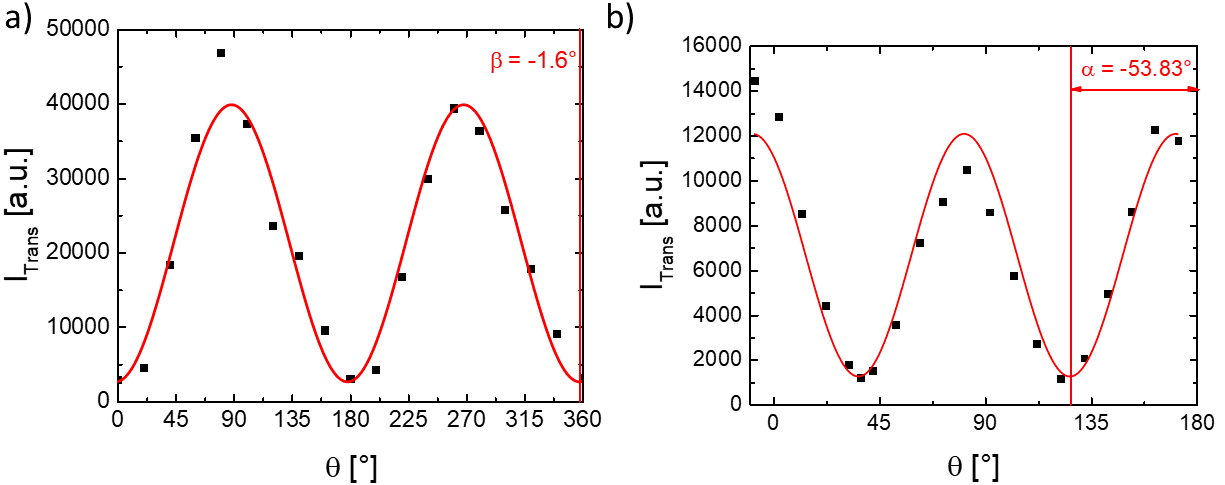
\includegraphics[width=1\textwidth]{Bilder/Methodik/OptElemente}
\caption{Darstellung a) der Transmissionskurve des Polarisators unter Verwendung
horizontal polarisierten Lichtes bei ursprünglich vertikal ausgerichteter
Transmissionsachse und b) der Transmissionskurve zweier gekreuzter Polarisatoren
mit $\uplambda$/4-Platte dazwischen. Beide Kurven wurden mit einer quadratischen
Sinusfunktion angepasst.} \label{OptElemente} \end{figure}Eine Anpassung mit
$\text{I}_\text{trans}=\text{sin}^2(\uptheta+ \upbeta)$ ergab eine Verschiebung
der Transmissionsachse um $\upbeta=(-\text{1.6}\pm \text{1.8})^\circ$ zur
Achsenkennzeichnung des Herstellers. Für die Vermessung der $\uplambda$/4-Platte
wurde ein zweiter Polarisator mit gekreuzter Transmissions- achse eingebaut.
Zwischen beide Polarisatoren wurde die $\uplambda$/4-Platte von 0$\ldots
$180$^\circ$ rotiert. Die Verschiebung der schnellen optischen Achse betrug
$\upalpha=(-\text{53.83}\pm\text{1.18})^\circ$ zur Achsenkennzeichnung des
Herstellers. In Ermangelung einer stabilen Laserquelle im Frequenzbereich der
Nanodrahtemission wurde auf eine Vermessung der Phasen- verschiebung verzichtet
und auf die Referenzwerte des Herstellers zurückgegriffen.\\ Durch die o.g.
Messungen müssen die Rechnungen der Stokes-Parameter korrigiert werden. Zunächst
die Verschiebung der Transmissionsachse: Unter Rotation der Transmissionsachse
um $\upbeta$ müssen sowohl die Gesamtintensität als auch der Polarsiationsgrad
der Strahlung erhalten bleiben. Da es sich um eine rotationssymmetrische
Transformation handelt, muss auch der S$_3$-Parameter inklusive des Drehsinn
erhalten bleiben. Für die Stokes-Parameter gilt also: \begin{equation} S_0&=A -
\frac{1+cos(\delta)}{1-cos(\delta)} \, C\text{ ,}\\ S_1&=
\frac{2}{1-cos(\delta)}\,\left[ C\, cos(2\,\beta) + D\,
sin(2\,\beta)\right]\text{ ,}\\ S_2&= \frac{2}{1-cos(\delta)}\,\left[ D\,
cos(2\,\beta) + C\, sin(2\,\beta)\right]\text{ ,}\\ S_3&=\frac{1}{sin(\delta)}
\, B \text{ ,} \label{StokesGL5} \end{equation} die für den Fall
$\upbeta=\text{0}^\circ$ und $\updelta=90^\circ$ in die \autoref{StokesGl4}
übergehen.\\ Die Verschiebung der $\uplambda$/4-Platte wird durch eine
Umsortierung der Einzelbilder um 67.5$^\circ$ korrigiert. Die verbleibende
Verdrehung kann auf $\uptheta$ addiert werden, sodass die Messung bei 8$^\circ$
statt bei 0$^\circ$ startet. Dies ist aufgrund des
Nyquist-Shannon-Abtasttheorems problemlos möglich.\\ In der Literatur finden
sich vereinzelnd abweichende Berechnungen des S$_\text{3}$-Parameters über einen
Sinus-Term \cite{Berry.1977,Anleitung}. Dies soll im Anhang kurz diskutiert und
falsifiziert werden (s. \autoref{StokesFalsch}). \subsection{Messablauf} Für
einen möglichst vollständigen Datensatz der einzelnen Nanodrahtes wurde die
PL-Emission für jeden Draht zunächst spektral vermessen und eine
Multimoden-Anpassung erstellt. Mithilfe des so ermittelten Laserschwellwertes
wurde der Anregungsbereich für die Folgemessungen auf das 1.2 - bis 2-fache
festgelegt. Anschließend wurden die Fourierabbildungen in nullter und erster
Beugungsordnung vermessen. Zunächst wurde die Gesamtintensität ohne Polarisator
und $\uplambda$/4-Platte ermittelt. Danach wurden die Messungen mit dem
Polarisator in vertikaler und horizontaler Ausrichtung wiederholt. Zum Schluss
wurde die $\uplambda$/4-Platte eingebaut und die Stokes-Parameter für beide
Fourier-Methoden vermessen. Die Messungen ohne und mit Polarisator dienen zur
Überprüfung der Messmethode der Stokes-Parameter, denn aus der Messung dieser
lassen sich die anderen drei Direktmessungen rekonstruieren – ergibt sich ein
konsistentes Bild, so wurde die Stokes-Messung korrekt ausgeführt. \\ Für die
magnetfeldabhängigen Messungen wurde das o.g. Schema in dieser Reihen- folge
jeweils ohne Magnetisierung und mit Magnetisierung orthogonal wie parallel zur
Nanodrahtachse hintereinander durchgeführt. Zusätzlich wurden die
Stokes-Parameter anhand des PL-Spektrums vermessen. Für die magnetfeldabhängige
Messung wurde das Spulenpaar für drei Sekunden mit 10.5 A betrieben und wieder
ausgeschaltet. Der Stromfluss wurde mit einem Digitalmultimeter (Peaktech 3325)
überprüft. \\ Es wurde während der gesamten Messungen streng darauf geachtet,
die Positionierung des Nanodrahtes nicht zu verändern und möglichst wenig mit
dem optischen Aufbau in Kontakt zu kommen. Da jedoch Polarisator und
$\uplambda$/4-Platte manuell ein- und ausgebaut sowie gedreht werden mussten,
war dies nur in begrenztem Rahmen möglich. So verschob sich in allen Messungen
das Substrat unter dem Laserspot und musste teils neu positioniert werden.
Zusätzlich verschiebt das Ein- und Ausschalten des Magnetfeldes die Position
geringfügig. Da sich mit der Verschiebung des Substrates Anregungsdichte und
Verstärkungsprofil des Drahtes verändern, war ein konsistentes Gesamtbild also
nur bedingt möglich. Innerhalb der Messungen einer Messmethode kann jedoch das
Bild als schlüssig betrachtet werden, da sich der Gesamtzyklus aller Messungen
und damit der Verschiebung über Stunden hinzieht. Nach Vermessung der optischen
Eigenschaften der Drähte wurden Länge und Durchmesser im
Rasterelektronenmikroskop (engl. \textit{scanning electron microscope}, kurz
\textit{SEM}) bestimmt. \subsubsection{Test der Methode} Um zu demonstrieren,
dass sich die Messmethode eignet, die Stokes-Parameter zu ermitteln, soll im
Folgenden exemplarisch die nullte Beugungsordnung eines \mbox{Nanodrahtes}
überprüft werden. Hierzu wurden sowohl die (rekonstruierten) Gesamtintensitäten,
als auch die aus \autoref{StokesGl6} und \autoref{StokesGl7} rekonstruierten
Intensitäten I$_\text{x}$ und I$_\text{y}$ mit Direktmessungen des Polarisators
mit horizontal bzw. vertikal orientierter Transmissionsachse verglichen. Aus
\autoref{S0_reconstruct_SiO2_S1_6} wird ersichtlich, dass die Gesamtintensitäten
durch den Einbau des Polarisators reduziert werden, die Charakteristika der
Bilder stehen jedoch in sehr guter Übereinstimmung zueinander. Zwischen den
Bildern jeweils vertikaler und horizontaler Feldelemente in
\autoref{horvert_reconstruct_SiO2_S1_6} gibt es nahezu keine Unterschiede.
Insbesondere wird dies durch Betrachtung der Differenzen zu \autoref
{Diff_SiO2_S1_6} deutlich, die zwar um den Nullpunkt schwanken, was zu großen
Teilen durch eine leichte Verschiebung der Bilder gegen- einander (durch das
Fehlen der $\uplambda$/4-Platte, bzw. der Drehung des Polarisators) und aus
Fluktuationen der Hintergrundstrahlung zu erklären ist. Folglich kann die
Messung der Stokes-Parameter als konsistent betrachtet werden. Selbige Tests
wurden mit allen Messungen dieser Masterthesis vollzogen. \begin{figure}[h]
\centering
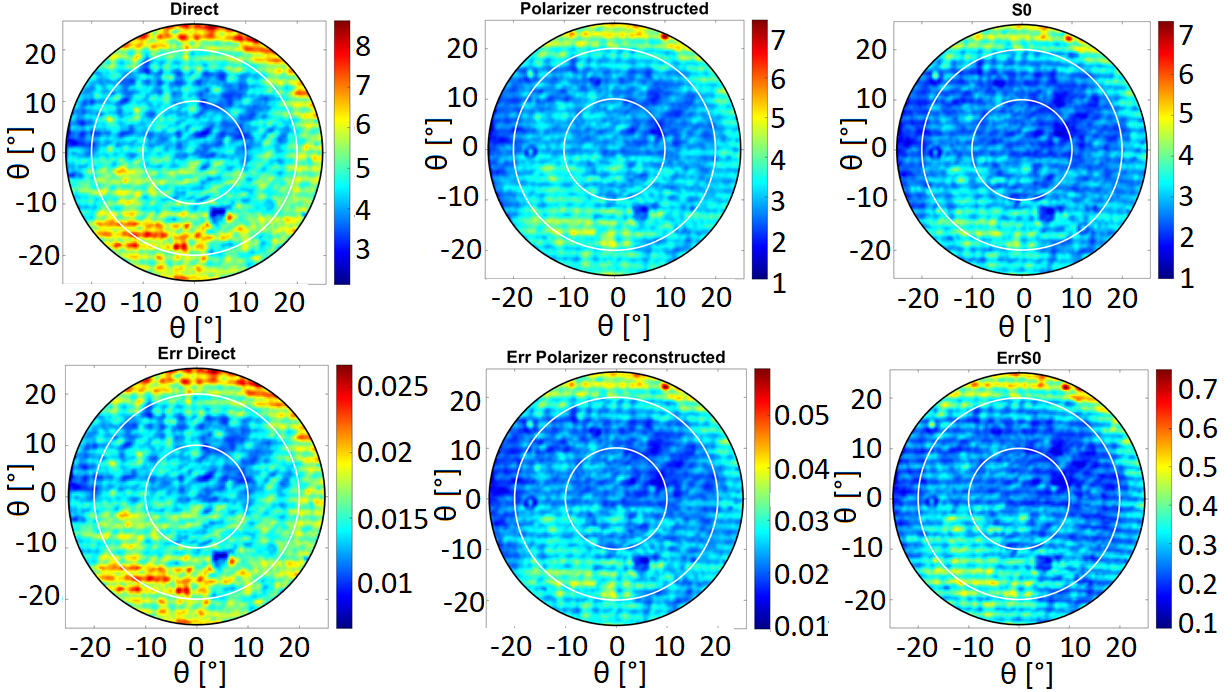
\includegraphics[width=.75\textwidth]{Bilder/Methodik/S0_reconstruct_SiO2_S1_6}
\caption{Obere Reihe: Messung der Gesamtintensität des Fourierbildes, direkt und
als Rekonstuktion der Intensitäten des Polarisators mit horizontal und vertikal
ausgerichteter Transmissionsachse sowie als Rekonstruktion S$_0$ der Stokes
Parameter; jeweils in nullter Beugungsordnung. Untere Reihe: Die jeweiligen
absoluten Fehler (s. \autoref{Fehler}).} \label{S0_reconstruct_SiO2_S1_6}
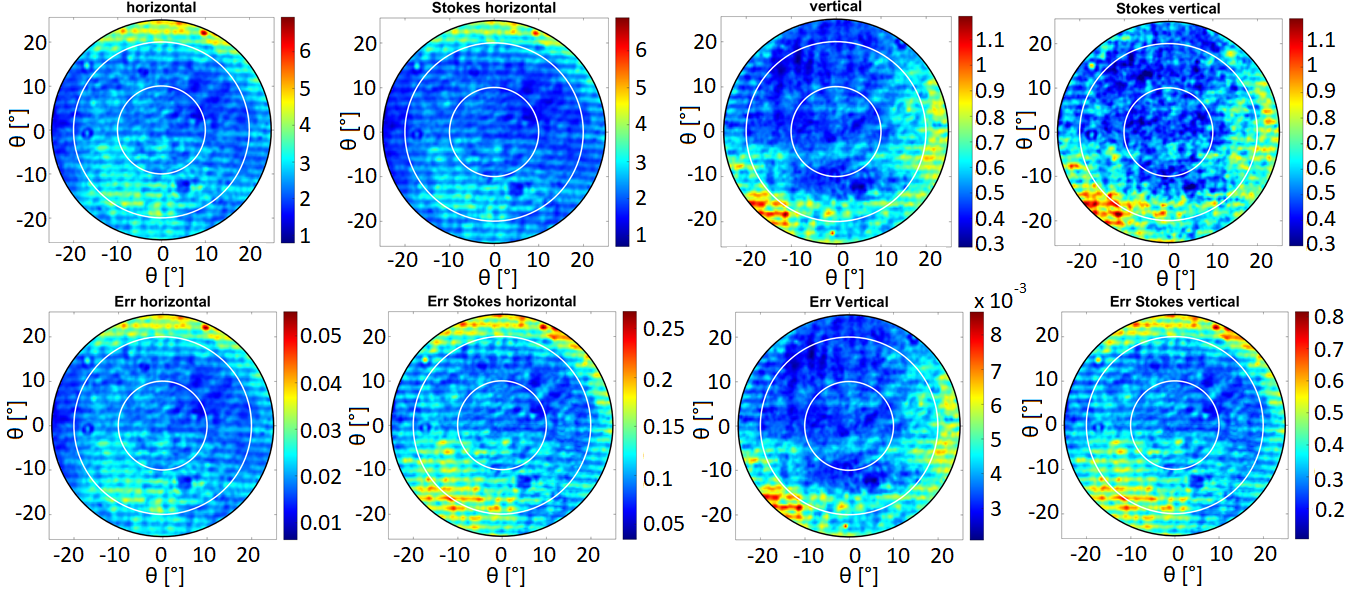
\includegraphics[width=1\textwidth]{Bilder/Methodik/horvert_reconstruct_SiO2_S1_6}
\caption{Obere Reihe: Messung der horizontalen und vertikalen Feldelemente des
Fourierbildes, mittels Polarisator sowie als Rekonstruktion der
Stokes-Parameter; jeweils in nullter Beugungsordnung. Untere Reihe: Die
jeweiligen absoluten Fehler.} \label{horvert_reconstruct_SiO2_S1_6} \centering
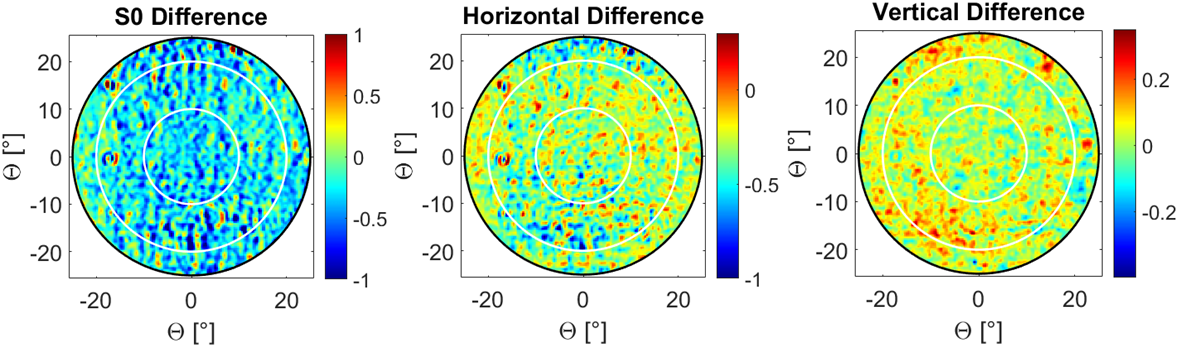
\includegraphics[width=.75\textwidth]{Bilder/Methodik/Diff_reconstruct_SiO2_S1_6}
\caption{Darstellung der Differenzen zwischen der über die Stokes-Parameter
rekonstruierten Intensitäten und der Polarisatormessungen aus
\autoref{S0_reconstruct_SiO2_S1_6} und \autoref{horvert_reconstruct_SiO2_S1_6}.}
\label{Diff_SiO2_S1_6} \end{figure} \chapter{Fourierabbildung der Emission von
ZnO-Nanodrähten} \section{ZnO-Nanodraht auf einem SiO$_\text{2}$-Substrat} Im
Folgenden soll die Emission eines Nanodrahtes auf einem SiO$_\text{2}$-Substrat
exemplarisch aufgearbeitet werden. Der untersuchte Draht ``SiO$_\text{2}$ 1''
war etwa 11 $\upmu$m lang, bei einem Durchmesser von etwa 395 nm (s.
\autoref{SEM_SiO2_S1_6}). Er zeigte einen Laserschwellwert bei \mbox{$\approx$
130 kW/cm$^\text{2}$} und wurde bei etwa 1.3-fachem Laserschwellwert untersucht
(s. \autoref{Cas_SiO2_S1_6} a)). Es zeigen sich vier Fabry-Pérot-Moden, von
denen die zweite Mode dominant gegenüber den anderen erscheint. Die erste und
letzte Mode sind klein und in ihrer Intensität ungefähr gleich stark ausgeprägt
(s. \autoref{Cas_SiO2_S1_6} b)).\begin{figure}[h] \centering
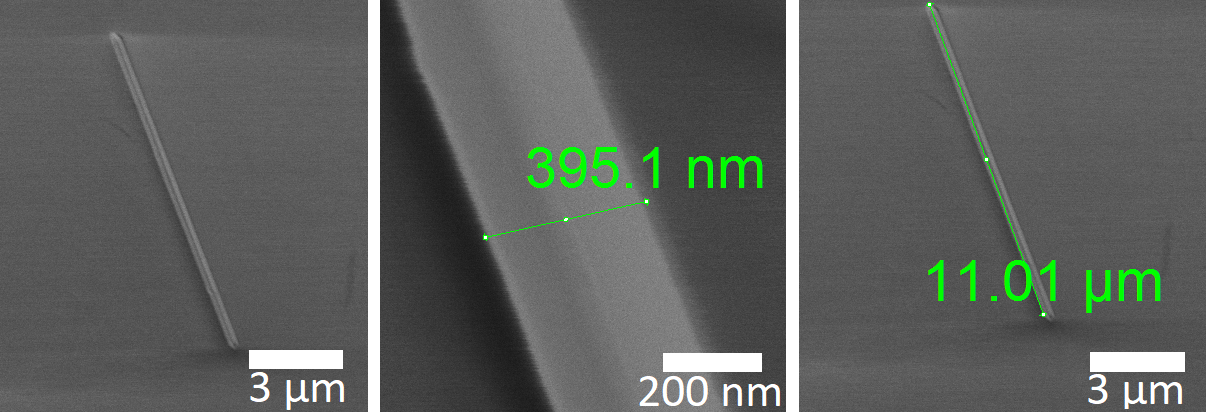
\includegraphics[width=.6\textwidth]{Bilder/SiO2/SEM_SiO2_S1_6}
\caption{REM-Bilder des Nanodrahtes mit der Länge \mbox{$\text{l} \approx
\text{11 }\upmu\text{m}$} und dem Durchmesser \mbox{$\text{d} \approx \text{395
nm}$} bei verschiedenen Vergrößerungen.} \label{SEM_SiO2_S1_6}
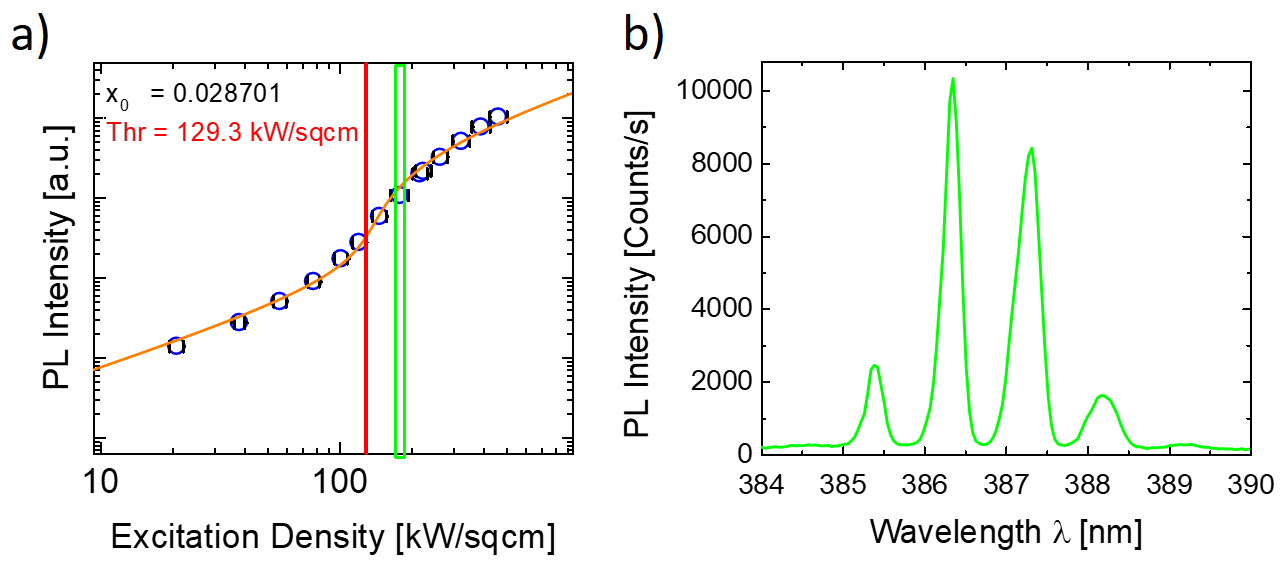
\includegraphics[width=.6\textwidth]{Bilder/SiO2/Cas_SiO2_S1_6} \caption{a)
Integrierte PL-Intensität des Nanodrahtes ``SiO$_\text{2}$ 1'' aus
\autoref{SEM_SiO2_S1_6} als Funktion der Anregungsleistung. Die durchgezogene
Linie zeigt die Multimoden-Anpassung des Nanodrahtes mit eingezeichneter
Schwellwert-Intensitätsdichte (rot) und Anregungsbereich der Fouriermessungen
(grün). b) Spektrum bei 1.3- fachem Laserschwellwert (175 kW/cm$^\text{2}$) und
Spaltbreite von 200 $\upmu$m.} \label{Cas_SiO2_S1_6} \end{figure}Aus dem
gemittelten Modenabstand der Fabry-Pérot-Moden lässt sich, nach Umstellung der
Resonanzbedingung \autoref{ResBed}, die Dispersion
$\frac{\text{dn}}{\text{d}\uplambda}$ zu \begin{equation}
\frac{dn}{d\lambda}=\frac{\left(n -\frac{\lambda^2}{2L\,
\Delta\lambda}\right)}{\lambda} = -(13.26 \pm 0.75)\, \upmu m^{-1} \text{ ,}
\label{Disp} \end{equation} mit dem Modenabstand $\Updelta\uplambda=$ 0.94 nm,
der zentralen Wellenlänge $\uplambda=$ 386.8 nm und dem \mbox{Brechungsindex} n
$=$ 2.1 für ZnO bei Hochanregung \cite{Wille.2016} errechnen. Dieser Wert liegt
zwischen den Literaturwerten von $\frac{\text{dn}}{\text{d}\uplambda}=$ -15
$\upmu$m$^\text{-1}$ \cite{O.Madelung.1984} und
$\frac{\text{dn}}{\text{d}\uplambda}=$ -12 $\upmu$m$^\text{-1}$
\cite{Zimmler.2010} und erscheint plausibel. Die Dispersion wird für
weiterführende Rechnungen auf dem MgO/Co/SiO$_\text{2}$ - Substrat benötigt und
soll hier näherungsweise als konstant für alle ZnO-Nanodrähte bei Hochanregung
gelten, denn nur für das SiO$_\text{2}$-Substrat konnte ein passender
Brechungsindex gefunden werden. \subsection{Fourierabbildung der
Nanodrahtemission} \subsubsection{Fourierabbildung in nullter Beugungsordnung}
Das Fourierbild der Laseremission des Nanodrahtes in \autoref{S0_S1_Si02_6} a)
zeigt die Intensitätsverteilung in Abhängigkeit vom Abstrahlwinkel, b) zeigt den
dazugehörigen absoluten Fehler. Eine ausführliche Fehlerbetrachtung findet sich
im Anhang in \autoref{Fehler}. Es lässt sich erkennen, dass die Emission für
größere vertikale Raumwinkel und somit in Richtung der Endfacetten zunimmt.
Deutlich sind horizontale Streifenmuster ausgebildet, die durch die Young'sche
Interferenz der beiden Facettenenden des Nanodrahtes entstehen und am Rand der
Abbildung leicht ``abknicken''.\begin{figure}[h] \centering
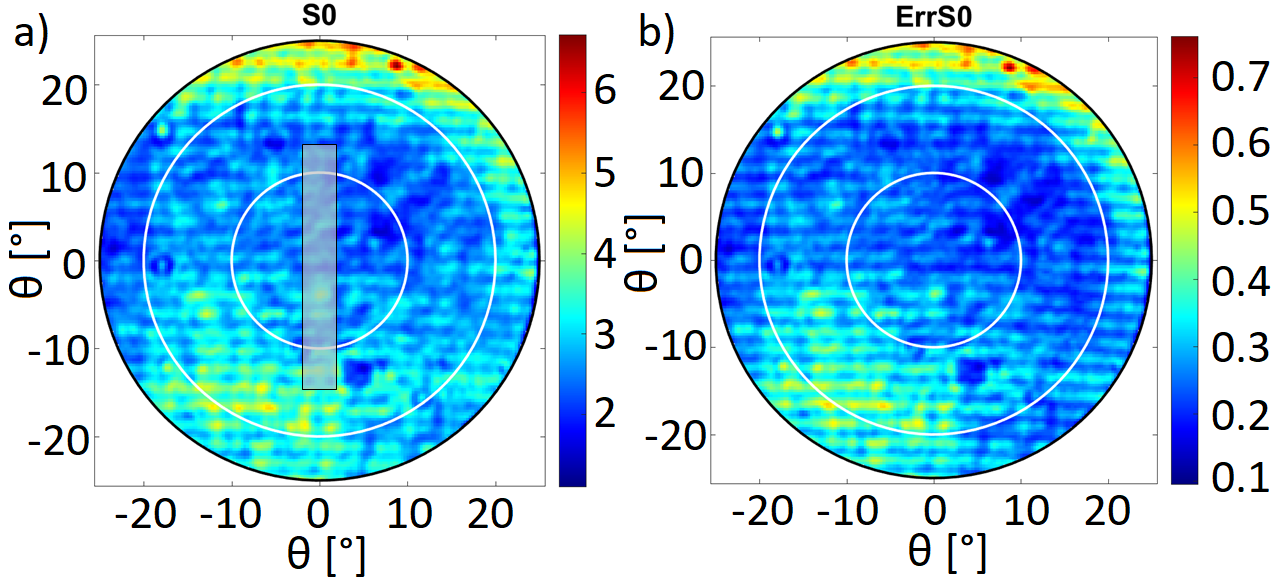
\includegraphics[width=.55\textwidth]{Bilder/SiO2/S0_S1_Si02_6} \caption{a)
Darstellung des S$_\text{0}$-Paramters des Drahtes ``SiO$_\text{2}$ 1'' aus
\autoref{SEM_SiO2_S1_6} in nullter Beugungsordnung bei 1.3-facher
Schwellintensitätsdichte. Der graue Balken repräsentiert die Orientierung des
Nanodrahtes orthogonal zum Interferenzmuster. b) Der absolute Fehler des
S$_\text{0}$-Parameters.} \label{S0_S1_Si02_6} \end{figure} Ein Blick in die
Linienprofile in \mbox{\autoref{Vert_Linescan_SiO2_S1_6} a) und b)} bei
verschiedenen horizontalen Raumwinkeln verdeutlicht diese Beobachtung. Bei den
Linienprofilen wurden die Basislinien subtrahiert, um die Phasenbeziehungen der
Linienprofile deutlicher darzustellen. Sie zeigen also nicht die direkte
Intensitätsverteilung, sondern nur die Intensität des Interferenzmusters über
dem Hintergrund. Die Linienprofile in \autoref{Vert_Linescan_SiO2_S1_6} a)
zeigen, dass die Maxima und Minima bei den gleichen vertikalen Raumwinkeln
phasengleich liegen, die horizontalen Raumwinkel ab $\text{16}^\circ$ hingegen
sind leicht verschoben, wie der Vergleich in \autoref{Vert_Linescan_SiO2_S1_6}
b) verdeutlicht.\begin{figure}[b]
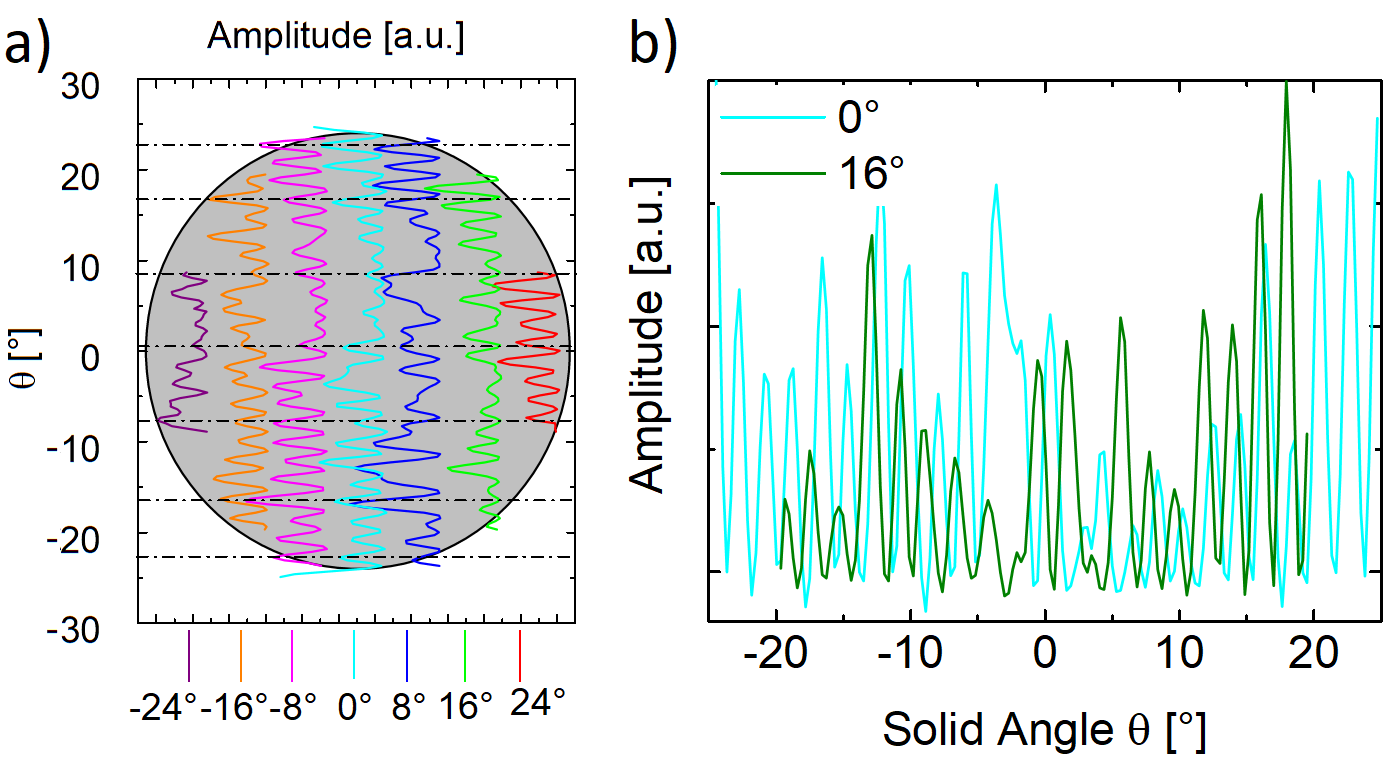
\includegraphics[width=.7\textwidth]{Bilder/SiO2/Vert_Linescan_SiO2_S1_6}
\caption{Darstellung der a) vertikalen Linienscans über 5 Pixel von -24$^\circ
\ldots \text{24}^\circ$ aus der Zweidimensionalen Messung, die in
\autoref{S0_S1_Si02_6} dargestellt ist, abzüglich der Basislinie und b) die
gegeneinander verschobenen Phasen der vertikalen Linienprofile bei 0$^\circ$ und
16$^\circ$.} \label{Vert_Linescan_SiO2_S1_6} \end{figure} Das Abknicken der
Moden am Rand könnte einen Hinweis auf das Vorliegen einer transversalen HE-Mode
sein \cite{Saxena.2015}. Die Fouriertransformation (engl. \textit{fast fourier
transformation}, kurz \textit{FFT}) in \autoref{FFT_Linescan_SiO2_S1_6} a) zeigt
jedoch bei allen vertikalen Raumwinkeln eine gleiche dominierende Frequenz. Über
die ermittelte Frequenz des Musters lässt sich bestätigen, dass es sich hierbei
um eine Interferenz nach dem Young'schen Doppelspaltexperiment handelt, bei der
die Emissionen aus den Endfacetten des Nanodrahtes interferieren, denn es ergibt
sich rechnerisch für die Nanodrahtlänge d: \begin{equation}
d=\frac{\lambda}{tan(1/f)}=(10.7 \pm 0.5) \, \mu m \text{ ,} \label{Distance}
\end{equation} mit der mittleren Wellenlänge der Fabry-Pérot-Moden $\uplambda=
\text{386.7}$ nm und der Frequenz von 0.48 1/$^\circ$. Ein Vergleich mit der
Bestimmung der Länge aus den elektronenmikroskopischen Aufnahmen (s.
\autoref{SEM_SiO2_S1_6}) des Nanodrahtes von $\text{d}\approx \text{11}\upmu
\text{m}$ steht somit in guter Übereinstimmung zur Rechnung. Das Vorhandensein
eines Interferenzmusters bedingt, dass es sich bei der Modenemission um
kohärentes Licht handelt. Eine FFT-Analyse von Linienprofilen in horizontaler
Richtung nach gleichem Muster (s. \autoref{FFT_Linescan_SiO2_S1_6} b)) zeigt
keine dominante Frequenz für verschiedene vertikale Raumwinkel. Die horizontalen
Modulationen der Intensität sind folglich nicht periodischer Natur, sondern
liegen in Abbildungsfehlern und Rauschen begründet. \begin{figure}[t]
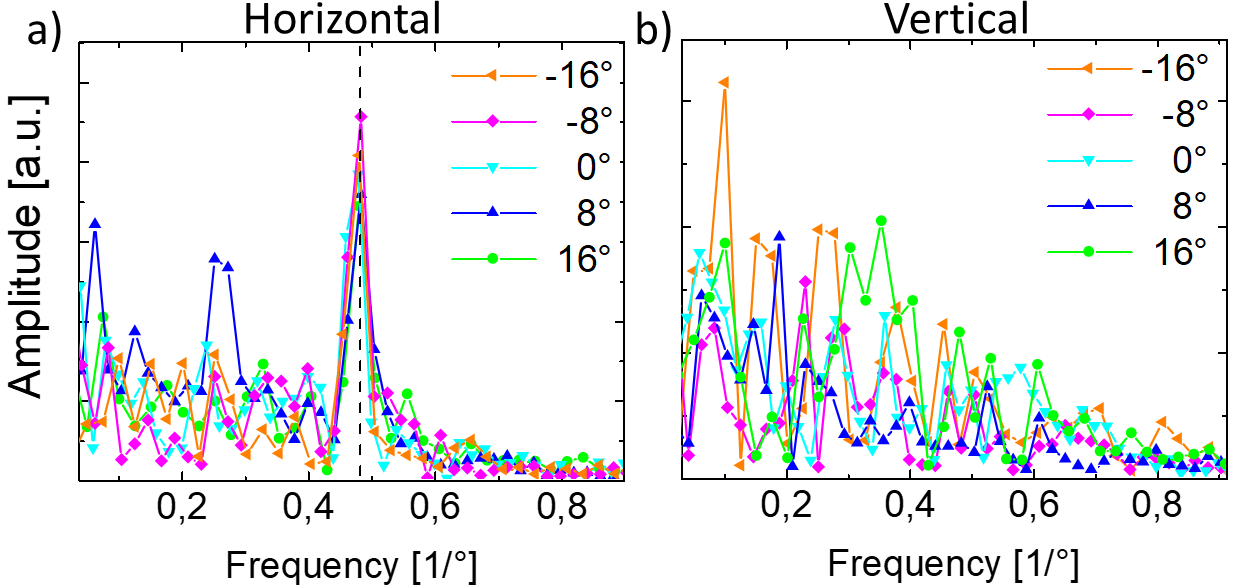
\includegraphics[width=.66\textwidth]{Bilder/SiO2/FFT_Linescan_SiO2_S1_6}
\caption{Fouriertransformation der Profile a) der vertikalen Profile aus
\autoref{Vert_Linescan_SiO2_S1_6}, mit einer dominierenden Frequenz von 0.48
1/$^\circ$, sowie b) der horizontalen Profile, ohne eine ausgezeichnete
Frequenz.} \label{FFT_Linescan_SiO2_S1_6} \end{figure} \subsubsection{Spektral
aufgelöste Fourierabbildung} Da das Signal-Rausch-Verhältnis in den
vorangegangen integralen Untersuchungen relativ klein ist, wurden die
Fouriermessungen der Emissioncharakteristik des \mbox{Nano}drahtes zusätzlich
spektral aufgelöst untersucht. Hierbei werden die einzelnen \mbox{Longitudinal-}
moden separiert und lassen sich getrennt voneinander betrachten. Dies wurde für
den in \autoref{SEM_SiO2_S1_6} gezeigten Nanodraht ``SiO$_\text{2}$ 1'' für drei
Abschnitte der vertikalen Raumwinkel wiederholt (s.
\autoref{S0_Spec_S1_Si02_6}). Wie erwartet steigt das Signal-Rausch-Verhältnis
und nahezu die komplette Intensität befindet sich hierbei in den Maxima des
Interferenzmusters der Moden; außerhalb der Moden erscheint die Intensität
gering. Im Folgenden wurde die Nummerierung der Moden nach \autoref{ModenNum}
gewählt. Vergleicht man benachbarte Moden, so zeigt sich eine Verschiebung des
Interferenzmusters um $\uppi$ (s. \autoref{Rec_Spec_S1_Si02_6} a)). Dies ist
eine direkte Konsequenz der Resonatorstruktur des Nanodrahtes. Damit eine Mode
resonant verstärkt werden kann, muss sie stehende Wellen ausbilden, folglich die
Resonanzbedingung \autoref{ResBed} erfüllen. Die Länge der Kavität muss also ein
ganzzahliges Vielfaches der halben Wellenlänge der Modenemission sein. Eine
benachbarte resonante Mode muss also um $\uppi$ in der Periode verschoben sein.
Summiert man die vertikalen Raumwinkel zu einem Spektrum auf (s.
\autoref{Rec_Spec_S1_Si02_6} c)), so zeigen sich im Vergleich zu
\autoref{Cas_SiO2_S1_6} b), aufgrund des breiteren\begin{figure}[h] \centering
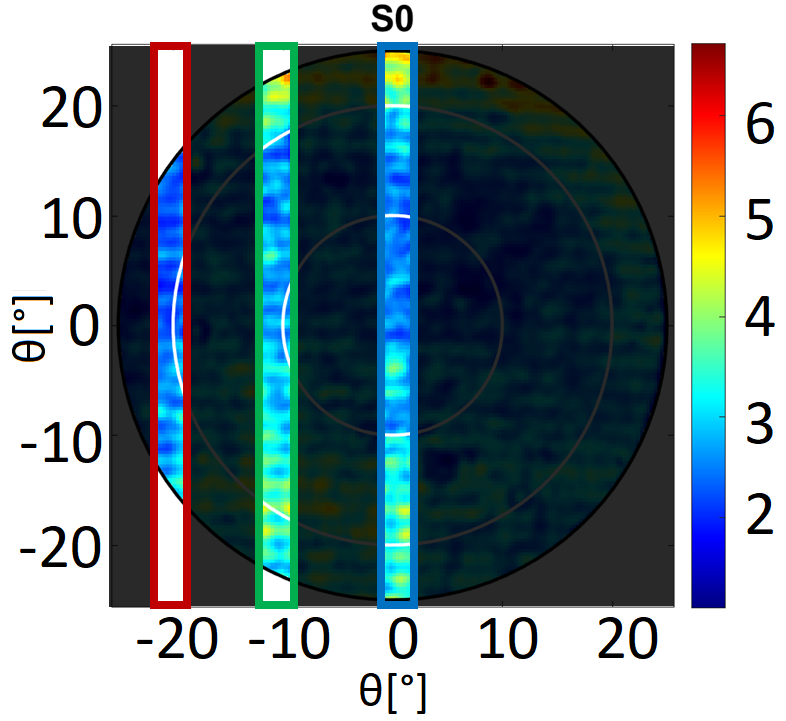
\includegraphics[width=.33\textwidth]{Bilder/SiO2/S0_Spec_1_S1_Si02_6}
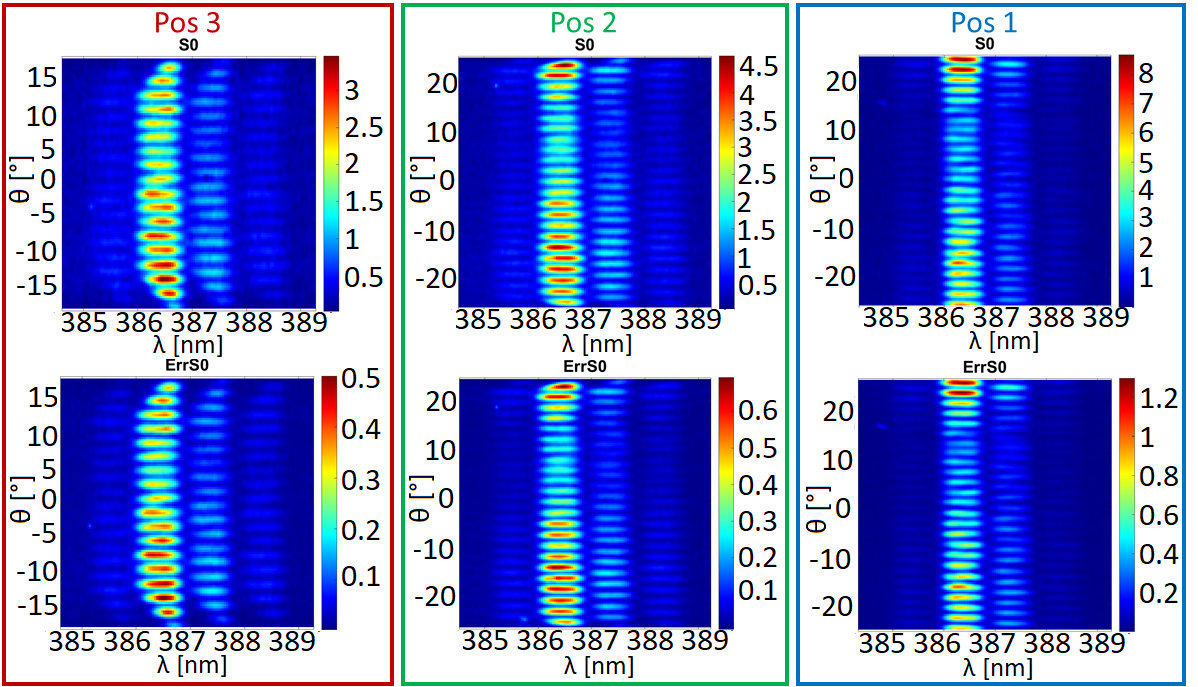
\includegraphics[width=.75\textwidth]{Bilder/SiO2/S0_Spec_S1_Si02_6}
\caption{Darstellung der spektral aufgelösten Fourierabbildung des Nanodrahtes
``SiO$_\text{2}$ 1'' aus \autoref{SEM_SiO2_S1_6} an den Positionen 1$\ldots$3
der vertikalen Raumwinkel mit den dazugehörigen absoluten Fehlern in der unteren
Reihe. Um die Verteilungen innerhalb eines Raumwinkels besser darzustellen, sind
die Skalierungen der Bilder unterschiedlich.} \label{S0_Spec_S1_Si02_6}
\end{figure}\begin{table}[h] \begin{tabular}{llll} Mode 1 & Mode 2 & Mode 3 &
Mode 4 \\ 385.4 nm & 386.4 nm & 387.3 nm & 388.3 nm \\ \end{tabular}
\caption{Nummerierung der Moden nach ihrer zentralen Wellenlänge $\uplambda$.}
\label{ModenNum} \end{table}\noindent Monochromatoreingangsschlitzes,
verbreiterte Moden. Zudem ist die Intensität der dritten Mode im Verhältnis zur
zweiten reduziert. Die Intensität fällt bei beiden Messmodi zu größeren
horizontalen Raumwinkeln ab (s. \autoref{Rec_Spec_S1_Si02_6}
d)).\begin{figure}[h]
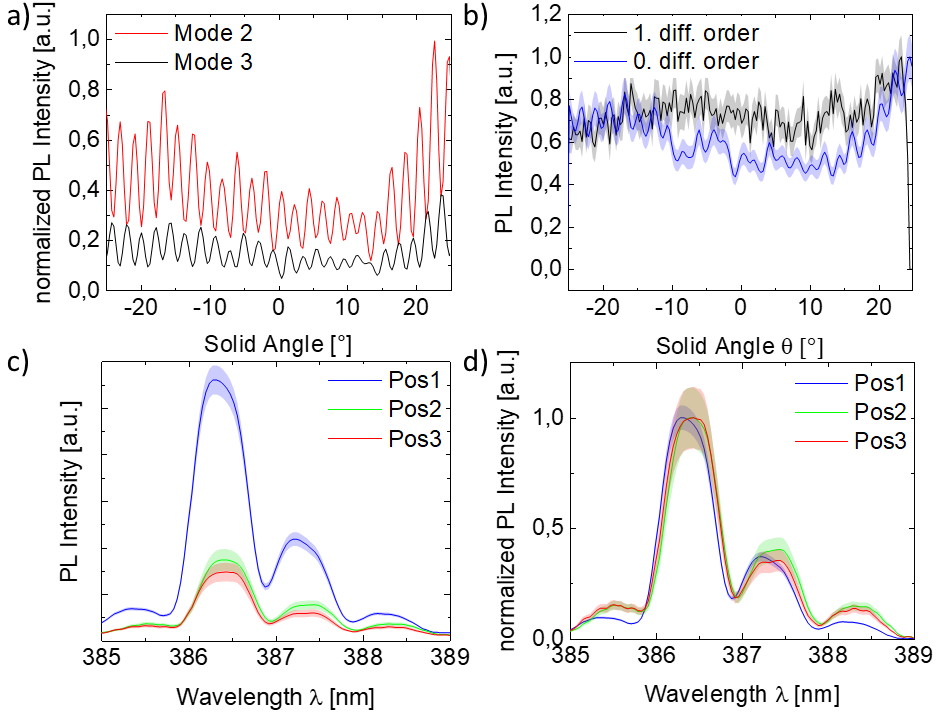
\includegraphics[width=.6\textwidth]{Bilder/SiO2/Rec_Spec_S1_Si02_6} \caption{a)
Linienprofil über die zweite und dritte Mode der spektral aufgelösten
Fourierabbildung an Position 1 (aus \autoref{S0_Spec_S1_Si02_6} extrahiert)
sowie b) Vergleich der 0. und 1. Beugungsordnung an der Position 1. Hierbei sind
in 0. Beugungsordnung das Linienprofil, sowie in 1. Beugungsordnung die Summe
über alle Wellenlängen dargestellt und auf 1 normiert. c) Summe über die
vertikalen Raumwinkel von -12.5$^\circ \ldots \text{12.5}^\circ$ an den
Positionen 1$\ldots$3 als Absolutwert und d) auf das jeweilige Maximum
normiert.} \label{Rec_Spec_S1_Si02_6} \end{figure}Hierbei betrifft der
Intensitätsverlust über die horizontalen Raumwinkel innerhalb der Messauflösung
alle Moden gleichermaßen, das heißt die Verhältnisse der Moden zueinander
bleiben konstant. Die Abstrahlcharakteristik für alle Moden eines Drahtes ist
also gleich. Summiert man über alle Wellenlängen, so ergibt sich für die
spektral aufgelösten Positionen 1$\ldots$3 jeweils der gleiche Trend wie für den
Bildausschnitt nullter Beugungsordnung (s. \autoref{Rec_Spec_S1_Si02_6} b)). Es
kann also festgehalten werden, dass der Kontrast des entstandenen
Interferenzmuster in nullter Beugungsordnung aus der Differenz zwischen der
Summe der ersten und dritten Longitudinalmode und der Summe der zweiten und
vierten Longitudinalmode entsteht. Die geraden und ungeraden Moden sind in ihrer
Phase um $\uppi$ verschoben und nur wenn ein Modenpaar dominiert, entsteht auch
in nullter Beugungsordnung ein Interferenzmuster.
\subsection{Polarisationseigenschaften der Nanodrahtemission}
\label{PolGradSiO2} \subsubsection{Polarisationsgrad der Nanodrahtemission}
Weitere Charakteristika der Nanodrahtemission sind die Polarisation und der
Polarisationsgrad der Strahlung. Der Anteil des polarisierten Lichtes ergibt
sich nach
$\text{I}_\text{Pol}=\sqrt{\text{S}_\text{1}^\text{2}+\text{S}_\text{2}^\text{2}+\text{S}_\text{3}^\text{2}}$
aus der Messung der Stokes-Parameter. In \autoref{Pol_SiO2_S1_6} sind die
Intensitätsverteilungen der Gesamtintensität $\text{S}_\text{0}$  und der Anteil
des davon polarisierten Lichtes des Drahtes ``SiO$_\text{2}$ 1'' aus
\autoref{SEM_SiO2_S1_6} in nullter Beugungsordnung gegenübergestellt. Beide
wurden nach dem Stokes-Formalismus berechnet. Es zeigen sich für die
Intensitäten beider Bilder ähnliche Verteilungen.\begin{figure}[b] \centering
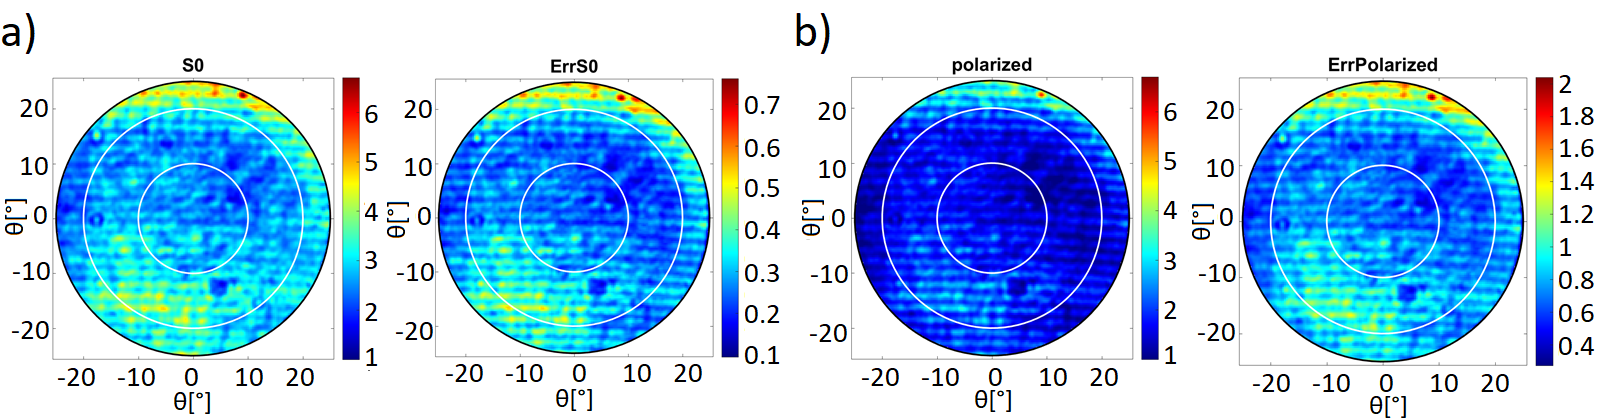
\includegraphics[width=1\textwidth]{Bilder/SiO2/Pol_SiO2_S1_6} \caption{Links:
Gegenüberstellung a) der Gesamtintensität mit b) dem polarisiertem Anteil der
Intensität, beide nach dem Stokes-Formalismus in nullter Beugungsordnung.
Rechts: Die jeweiligen absoluten Fehler.} \label{Pol_SiO2_S1_6} \end{figure}Um
eine qualitative Information über die Polarisation zu erlangen, muss die
Gesamtintensität herausgerechnet werden, sodass sich für jeden Pixel eine
Aussage über den Anteil der jeweilig polarisierten Strahlung an der
Gesamtintensität des Pixels treffen lässt – den Polarisationsgrad DOP. Für den
Polarisationsgrad wird also der Anteil des polarisierten Lichtes durch die
Gesamtintensität S$_\text{0}$ dividiert (s. \autoref{DOPStokes}). Es zeigt sich
in \autoref{DOP_SiO2_S1_6} a), dass der Polarisationsgrad zu den Endfacetten hin
zunimmt sowie für größere horizontale Winkel nachlässt. Zudem zeigen die Maxima
des Interferenzmusters einen deutlich erhöhten
Polarisationsgrad.\begin{figure}[b]
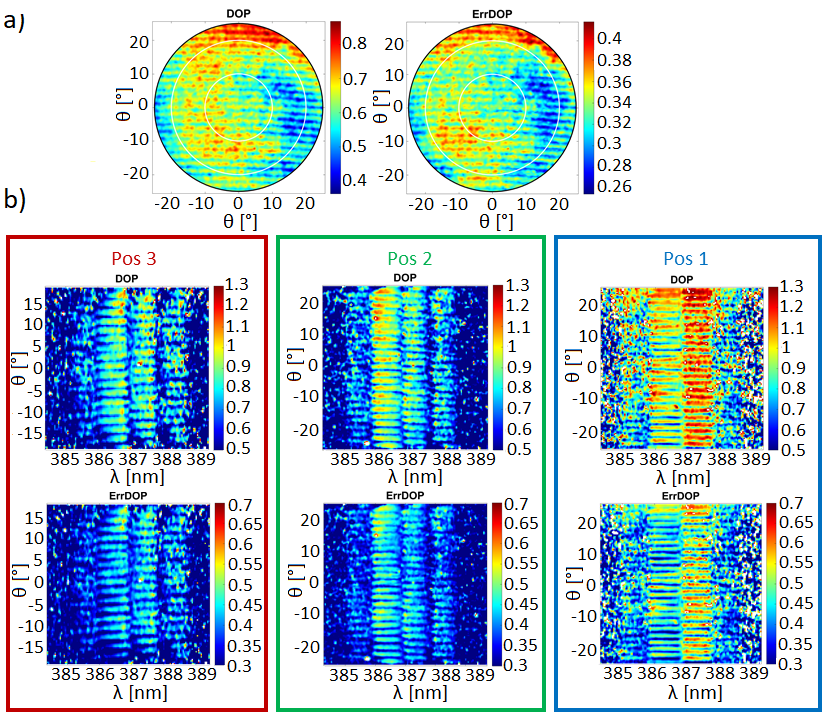
\includegraphics[width=0.75\textwidth]{Bilder/SiO2/DOP_SiO2_S1_6}
\caption{Darstellung des olarisationsgrades des Nanodrahtes ``SiO$_\text{2}$ 1''
aus \autoref{SEM_SiO2_S1_6} in a) nullter Beugungsordnung und b) Obere Reihe:
Darstellung der ersten Beugungsordnung an den Positionen 1$\ldots$3. Untere
Reihe: Die jeweiligen absoluten Fehler.} \label{DOP_SiO2_S1_6} \end{figure}Löst
man den Polarisationsgrad spektral an den Positionen 1$\ldots$3 auf (s.
\autoref{DOP_SiO2_S1_6} b)), zeigt sich, dass die Moden mit einem
Polarisationsgrad von DOP $\approx (\text{0.9}\pm\text{0.45})$ fast vollständig
polarisiert sind. Polarisationsgrade > 1 sind unphysikalisch und treten hier
aufgrund von Messungenauigkeiten auf, liegen aber innerhalb der errechneten
Fehlertoleranzen. Die leichten Unterschiede resultieren aus
Intensitätsunterschieden der Moden über der spontanen Emission und der ASE.
Entsprechend sind die erste und vierte Mode gegenüber den anderen beiden Moden
weniger stark polarisiert, sie folgen aber dem selben Verlauf über die
vertikalen Raumwinkel. Zusammen mit der erhöhten Intensität und der Kohärenz,
ist der hohe Polarisationsgrad der Modenemission eine Bestätigung ihrer Herkunft
aus einem Laserprozess.\\ Bei einem weiter gewählten Spektralbereich (s.
\autoref{compSpec_2_DOP}) wird deutlich, dass außerhalb der Moden, im Bereich
der NBE, der Polarisationsgrad DOP $\approx (\text{0.5} \pm \text{0.3})$
deutlich erhöht ist.\begin{figure}[h]
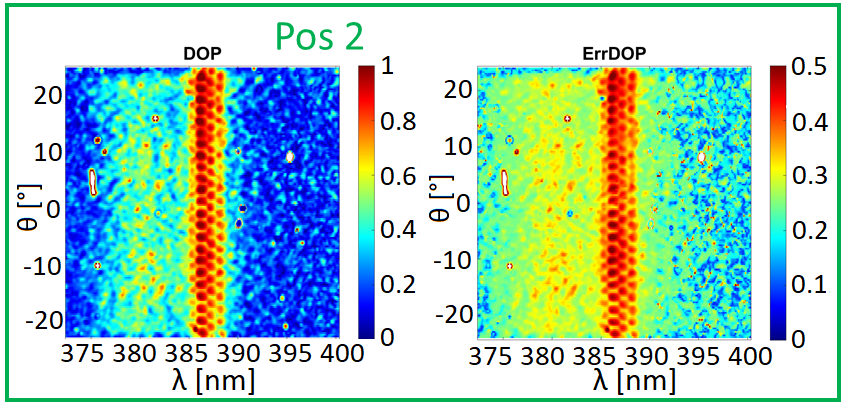
\includegraphics[width=.55\textwidth]{Bilder/SiO2/compSpec_2_DOP}
\caption{Darstellung der Position 2 aus \autoref{DOP_SiO2_S1_6} in einem
weiteren Spektralbereich mit absolutem Fehler.} \label{compSpec_2_DOP}
\end{figure}Es wäre jedoch für spontane Emission zunächst keine Polarisation zu
erwarten. Betrachtet man jedoch \autoref{spinueb}, so zeigt sich, dass für die
Exzitonen X$_\text{A}$ und X$_\text{B}$ der oberen beiden Valenzbänder die
Dipolübergänge mit horizontaler elektrischen Feldkomponente $\vec{\textbf{E}}
\bot \vec{\textbf{c}}$ dominieren. Das X$_\text{C}$ Exziton mit elektrischem
Feldvektor $\vec{\textbf{E}} \| \vec{\textbf{c}}$ liegt ungefähr 44 meV über der
Energie der anderen beiden Exzitonen. Dieser Übergang ist also
unwahrscheinlicher, sodass die NBE von den ersten beiden horizontal
polarisierten Exzitonenübergängen dominiert wird. Dieses gilt nach Jacopin et
al. (2011) \cite{Jacopin.2011} auch bei Raumtemperatur; die publizierten
Polarisationsgrade der NBE von ungefähr DOP $\approx \text{63}$\% bei
Raumtemperatur decken sich mit denen in dieser Masterthesis gezeigten und auch
die horizontale Polarisation der NBE kann an späterer Stelle bestätigt  werden.
Deutliche Ausschläge einzelner Pixel hin zu sehr hohen Polarisationsgraden sind
hier, aufgrund der geringen Statistik, dem Hintergrundrauschen (s. Anhang
\autoref{Rauschen}) geschuldet.\\ Zusammen mit \autoref{S0_Spec_S1_Si02_6} wird
also klar, warum der Polarisationsgrad in \autoref{DOP_SiO2_S1_6} a) zu den
Endfacetten zunimmt und zu höheren horizontalen Raumwinkeln abnimmt: Vor dem
Hintergrund einer homogen verteilten spontanen Emission entscheidet die
Intensität der Moden über den Gesamtpolarisationsgrad. Da diese Modenemission
durch die Geometrie des Nanodrahtes vornehmlich zu hohen vertikalen Raumwinkeln
zunimmt, hingegen zu hohen horizontalen Raumwinkeln abnimmt (s.
\autoref{S0_S1_Si02_6}), folgt der Polarisationsgrad dem Trend der
Intensitätsverteilung, da diese maßgeblich von der Intensitätsverteilung der
Modenemission herrührt (s. \autoref{Rec_Spec_S1_Si02_6} b)).
\subsubsection{Stokes-Parameter der Polarisation} Neben der
Intensitätsverteilung und dem Polarisationsgrad ist vor allem auch die Art der
Polarisation von Relevanz. Diese wird durch die Stokes-Parameter
$\text{S}_{\text{1} \ldots \text{3}}$ beschrieben (s.
\autoref{IntroStokesParams}). Im Folgenden wurden die Stokes-Parameter des
Nanodrahtes ``SiO$_\text{2}$ 1'' aus \autoref{SEM_SiO2_S1_6} auf den Anteil des
polarisierten Lichtes normiert und sind mit einem ``p'' hinter dem jeweiligen
Parameter gekennzeichnet. Diese Normierung hat den Vorteil, dass sich das
Verhältnis der Stokes-Parameter zueinander schneller erfassen lässt. Die
Informationen über Intensitätsverteilung sowie Anteil polarisierten Lichtes
(samt ihrer Fehler) werden hier also ausgeklammert, da sie bereits in den
vorherigen Abschnitten beschrieben wurden, und nur die Verhältnisse der
Stokes-Parameter zueinander betrachtet werden sollen.\begin{figure}[b]
\centering 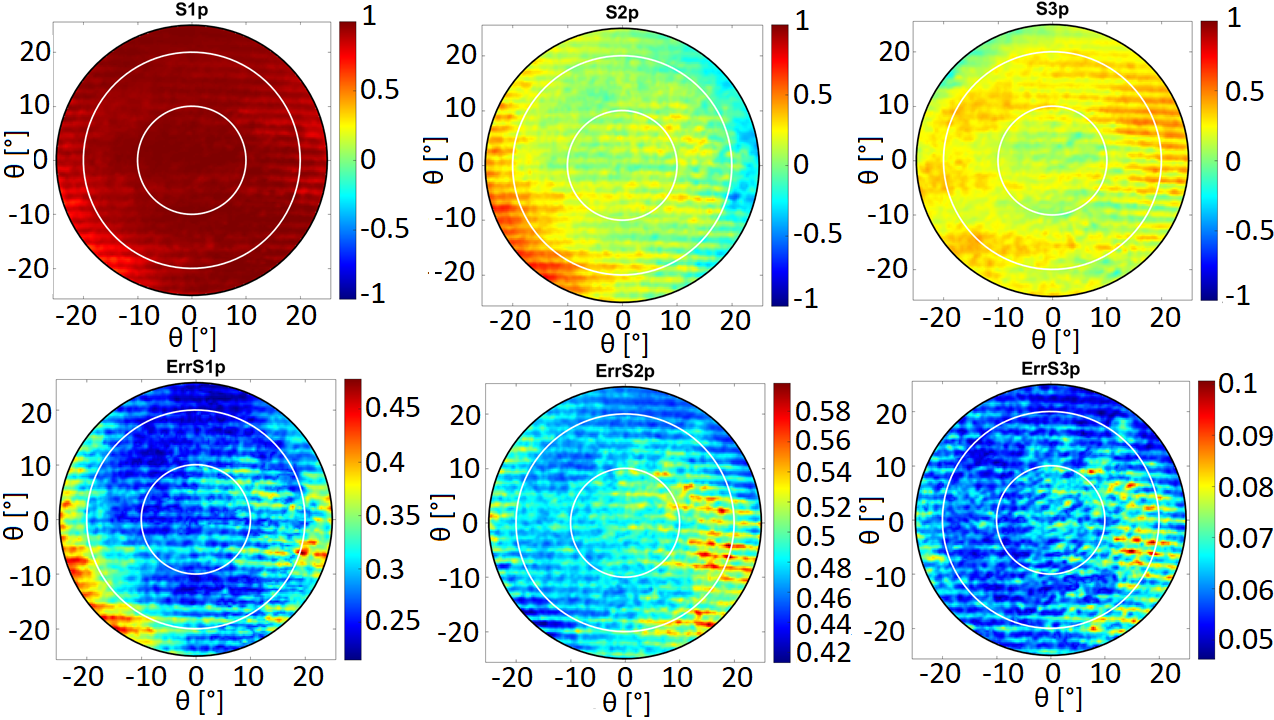
\includegraphics[width=0.66\textwidth]{Bilder/SiO2/StokesP_S1_Si02_6}
\caption{Obere Reihe: Dartellung der auf den polarisierten Anteil der Emission
normierten Stokes-Parameter des Nanodrahtes ``SiO$_\text{2}$ 1'' aus
\autoref{SEM_SiO2_S1_6} in nullter Beugungsordnung. Zur besseren
Vergleichbarkeit sind die Stokes-Parameter gleich skaliert. Untere Reihe: Die
jeweiligen absoluten Fehler.} \label{StokesP_S1_SiO2_6} \end{figure}Die
Gegenüberstellung der Stokes-Parameter in nullter Beugungsordnung in
\autoref{StokesP_S1_SiO2_6} zeigt, dass der $\text{S}_\text{1,p}$-Parameter, der
den Anteil horizontal linear polarisierten Lichtes wiedergibt, für fast alle
Raumwinkel dominiert und innerhalb der Fehler für alle Winkel in etwa konstant
ist. Für höhere horizontale Raumwinkel nimmt der $\text{S}_\text{1,p}$-Parameter
leicht ab; an diesen Stellen zeigen sich jedoch auch die größten Fehler.\\ Der
Anteil des S$_\text{2,p}$-Parameters, der den um 45$^\circ$ gegenüber der
Horizontale gekippten Anteil linear polarisierten Lichtes beschreibt, verhält
sich genau entgegengesetzt und nimmt betragsmäßig für höhere horizontale
Raumwinkel zu, je nach Seite aber mit unterschiedlichem Vorzeichen. Er liegt für
große Teile der Raumwinkel unterhalb seine Fehlertoleranz.\\ Für höhere
Raumwinkel sind zusätzlich auch kleinere, jedoch signifikante Anteile zirkular
polarisierten Lichtes vorhanden, die durch den S$_\text{3,p}$-Parameter
beschrieben werden. Das Vorzeichen gibt hier Auskunft über den Drehsinn.\\ Löst
man die Fourierabbildung spektral auf (s. \autoref{Spec_StokesP_S1_SiO2_6}),
zeigt sich auch hier ein ähnliches Bild. Der S$_\text{1,p}$-Parameter dominiert
für alle Raumwinkel. Es zeigen sich jedoch auch für den S$_\text{2,p}$- und
S$_\text{3,p}$-Parameter höhere Polarisationsgrade, diese liegen allerdings in
den Minima des Interferenzmusters (s. \autoref{SpecP1_StokesP_Line_S1_Si02_6}
a)). Betrachtet man den Wert der Stokes-Parameter an den Maxima des
Interferenzmusters, so ergeben sich ähnliche Werte wie in
\autoref{StokesP_S1_SiO2_6} an den entsprechenden Positionen. Obwohl die
Modenemission deutlich den Polarisationsgrad in nullter Beugungsordnung
dominieren sollte, sind die Unterschiede zwischen beiden messbar. Ursächlich
hierfür ist wahrscheinlich Polarisation der NBE (s. \autoref{compSpec_2_S1p}),
die sich in nullter Beugungsordnung mit den Stokes-Parametern der Moden
überlagert.\begin{figure}[b]
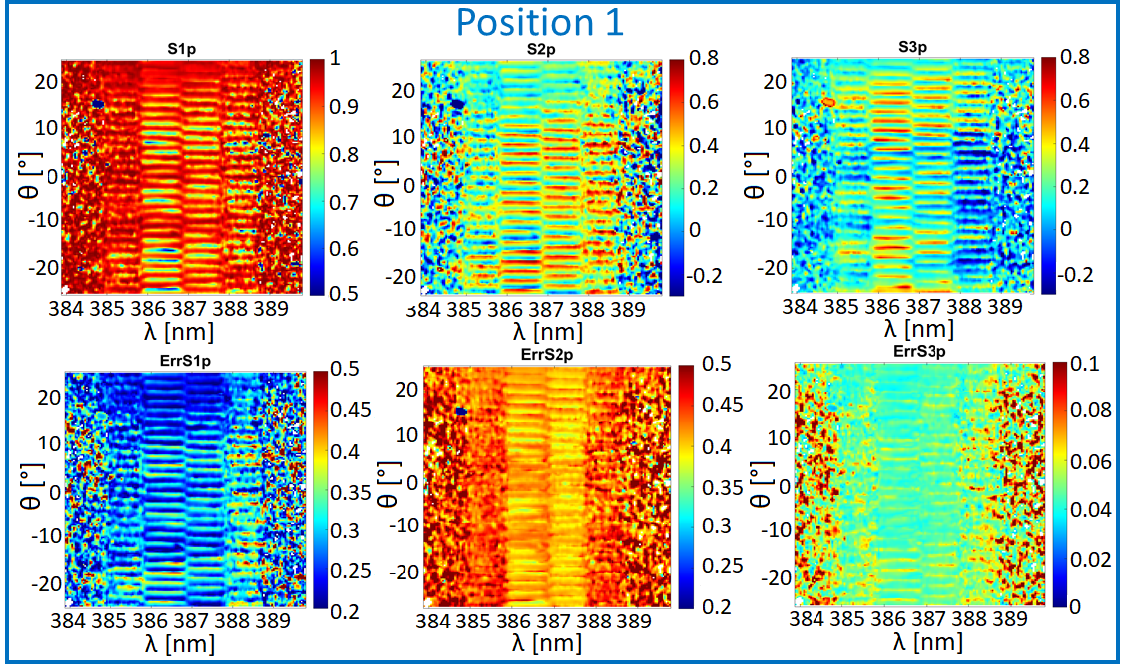
\includegraphics[width=0.66\textwidth]{Bilder/SiO2/SpecP1_StokesP_S1_Si02_6}
\caption{Obere Reihe: Darstellung der spektral aufgelösten und auf den
polarisierten Anteil der Emission normierten Stokes-Parameter des Nanodrahtes
aus \autoref{SEM_SiO2_S1_6} an Position 1. Zur besseren Übersicht über die
Verteilung sind die Stokes-Parameter unterschiedlich skaliert. Untere Reihe: Die
jeweiligen absoluten Fehler.} \label{Spec_StokesP_S1_SiO2_6}
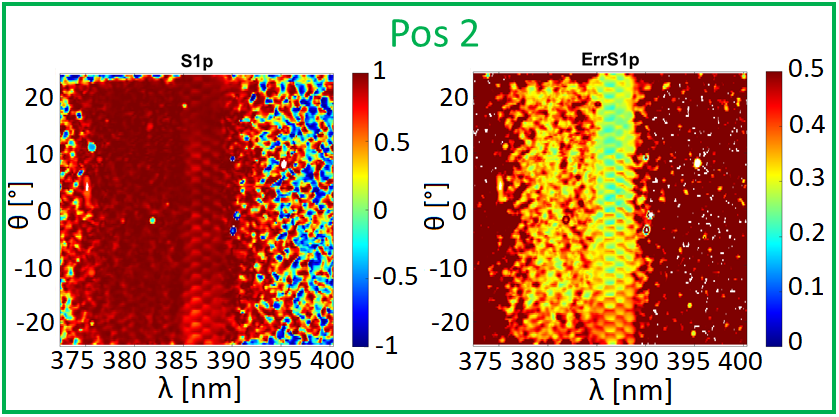
\includegraphics[width=0.5\textwidth]{Bilder/SiO2/compSpec_2_S1p}
\caption{Darstellung des S$_\text{1,p}$-Parameter eines weiter gefassten
Spektralbereiches an der Position 2 der \autoref{S0_Spec_S1_Si02_6}.}
\label{compSpec_2_S1p} \end{figure}Anhand des S$_\text{1,p}$-Parameters lässt
sich zeigen, dass die Polarisationsrichtung aller Moden sich über die vertikalen
Raumwinkel gleich verhält (s. \autoref{SpecP1_StokesP_Line_S1_Si02_6} b)). Ein
gleicher Polarisationsgrad und eine gleiche Intensitätsverteilung aller Moden
sind Indizien dafür, dass alle Longitudinalmoden des Nanodrahtes mit der
gleichen Transversalmode oder gleicher Überlagerung verschiedener
Transversalmoden schwingen. Der geringe Anteil des S$_\text{2,p}$-Parameters,
der zu höheren Raumwinkeln zunimmt, könnte ein Indiz für Randeffekte des
Objektivs sein. Auch Streuprozesse am Substrat könnten hierbei eine Rolle
spielen, die sich in einer Erhöhung des Untergrundes hinter dem
Interferenzmuster der Moden äußerten, da die Phasenbeziehung verloren ginge.
Dies ließe sich mit dieser Messmethode quantitativ jedoch nicht verifizieren.
Generell führt auch eine leichte Verkippung der Nanodrahtachse in der Bildebene
zu einer Erhöhung des S$_\text{2,p}$-Parameters.\\ Betrachtet man diese Effekte
und den großen Fehler des S$_\text{2,p}$-Parameters zusammen mit der Dominanz
des S$_\text{1,p}$-Parameters, so erscheint es sinnvoll den S$_\text{1,p}$- und
den S$_\text{2,p}$-Parameter zum linearen Polarisationsgrad (engl.
\textit{degree of linear polarization}, kurz \textit{DOLP}) zusammenzufassen (s.
\autoref{DOLP_S1_SiO2_6}). Der Anteil linearer Polarisation berechnet sich nach
$\text{I}_\text{Lin.
Pol}=\sqrt{\text{S}_\text{1}^\text{2}+\text{S}_\text{2}^\text{2}}$ und soll im
Folgenden wie die Stokes-Parameter auch auf den Gesamtanteil polarisierten
Lichtes genormt sein.\begin{figure}[b]
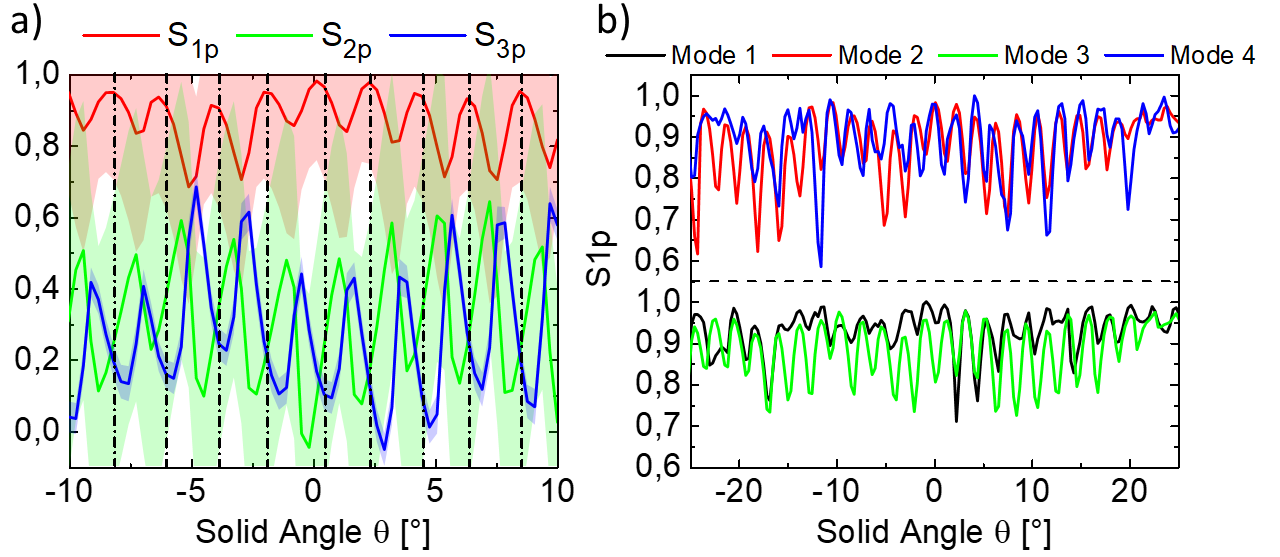
\includegraphics[width=.66\textwidth]{Bilder/SiO2/SpecP1_StokesP_Line_S1_Si02_6}
\caption{a) Profile der Stokes-Parameter aus \autoref{Spec_StokesP_S1_SiO2_6}
der zweiten Mode. Schwarz gestrichelt dargestellt sind die Positionen der
Interferenzmaxima der Gesamtintensität aus \autoref{S0_Spec_S1_Si02_6} an
gleicher Position und Mode. b) Profile des S$_\text{1,p}$-Parameters der vier
Moden aus \autoref{StokesP_S1_SiO2_6}. Zusammen dargestellt sind jeweils die
geraden und die ungeraden Moden.} \label{SpecP1_StokesP_Line_S1_Si02_6}
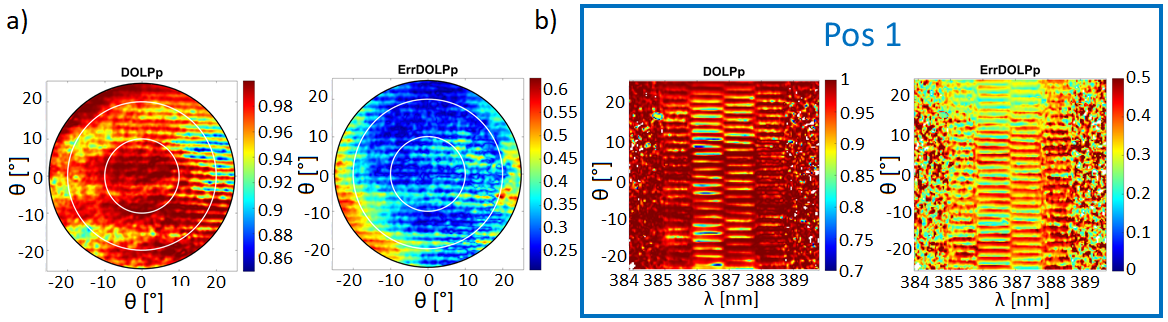
\includegraphics[width=1\textwidth]{Bilder/SiO2/DOLP_SiO2_S1_6} \caption{Links:
Darstellung des linearen Polarisationsgrades der Nanodrahtemission normiert auf
den Gesamtanteil polarisierten Lichtes in a) nullter Beugungsordnung und b)
spektral aufgespalten an Position 1. Rechts: Die jeweiligen absoluten Fehler.}
\label{DOLP_S1_SiO2_6} \end{figure} \\Damit zirkular polarisiertes Licht einer
Vorzugsrichtung aus Rekombinationsprozessen entstehen kann, muss in das
Materialsystem ein Drehimpuls eingebracht werden. Dies kann in Form von
Spin-Injektion, bspw. durch  das Pumpen eines Energieniveaus (s. \autoref{Ausw})
durch einen zirkular polarisierten Laser, kann aber auch durch externe Felder
erfolgen, die die Entartung des Leitungsbandes und der Valenzbänder aufheben.
Ohne diese externen symmetriebrechenden Elemente wären gleichverteilte Anteile
links- und rechtszirkular polarisierten Lichtes zu erwarten. Durch die
Definition des S$_\text{3}$-Parameters als Differenz der beiden Drehrichtungen
würde dieser Parameter verschwinden und als unpolarisiertes Licht in Erscheinung
treten. Anderweitige richtungsabhängige Trennungen der beiden Drehrichtungen in
Nah- und Fernfeld müssten durch Simulationen der Finite-Differenzen-Methode
\mbox{(engl. \textit{Finite-Difference-Time-Domaine},} kurz \textit{FDTD})
bestätigt oder ausgeschlossen werden. \\ Der verwendete Laser erzeugte linear
polarisiertes Licht, dennoch kann sich dieses  bei der Propagation durch den
Versuchsaufbau anteilig in zirkular polarisiertes Lichtes umwandeln. Diese
Anteile sind aber als gering zu betrachten und somit zu vernachlässigen. Selbst
unter ausschließlicher Verwendung zirkular polarisierten Lichtes wäre nur eine
Spinpolarisation von max. 1.5\% zu erwarten (s. Anhang \autoref{Spininjection}).
Da dieser Laser aber höchstens einen kleinen Teil zirkular polarisierten Lichtes
enthält, ist auch dieser Effekt zu vernachlässigen. \\ Das
SiO$_\text{2}$-Substrat besteht aus diamagnetischem Material und keine externen
Felder wurden bewusst angelegt. Es kann ein hintergründiges Störfeld am
Probenort durch Stromflüsse in den Instrumenten zwar nicht ausgeschlossen
werden, aufgrund anzunehmender geringer Feldstärken ist dieses aber
näherungsweise zu vernachlässigen. Das Entstehen zirkular polarisierten Lichtes
einer Vorzugsrichtung als Laserprozess ist folglich unwahrscheinlich, da kein
externer Drehimpuls eingebracht wird.\\ ZnO ist ein doppelbrechendes
Materialsystem. Linear polarisiertes Licht könnte von den unterschiedlichen
Brechungsindizes parallel und orthogonal zur c-Achse (s. \autoref{ZnOMat})
beeinflusst werden – es entstünde somit ein Anteil zirkular polarisierten
Lichtes. Da sich das Materialsystem in Hochanregung befindet, verändern sich die
Brechungsindizes \cite{Wille.2016}. Dieser Anteil sollte also verglichen mit der
Dominanz der Transversalmoden keine Rolle mehr spielen.\\ Weitere Möglichkeiten
wären Effekte der optischen Elemente nach der Emission, die zur zirkularen
Polarisation führen könnten. Diesbezüglich müsste jede optische Komponente
ausgemessen werden. Die Herkunft des S$_\text{3,p}$-Parameters kann also an
dieser Stelle nicht abschließend geklärt werden und mag aus einer Überlagerung
der verschiedenen oben genannten Effekte resultieren.\\ Die Polarisation der
Endfacettenemission des Nanodrahtes wird insgesamt stark von der horizontalen
linearen Polarisation dominiert, die Parameter S$_\text{2,p}$ und S$_\text{3,p}$
treten dabei in den Hintergrund. Relativ zur Substratoberfläche wird die
Polarisationsrichtung zur Veranschaulichung in \autoref{PolPic} schematisch
dargestellt.\begin{figure}[b] \centering
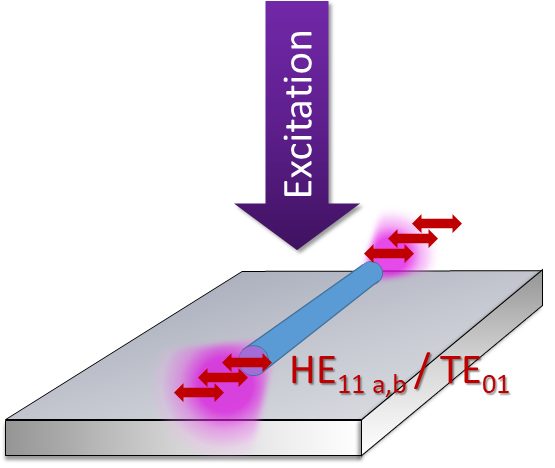
\includegraphics[width=.35\textwidth]{Bilder/SiO2/PolPic} \caption{Schematische
Darstellung der horizontalen Polarisationsrichtung der Laseremission des
Nanodrahtes auf einem SiO$_\text{2}$-Substrat.} \label{PolPic} \end{figure}Ein
Blick in \autoref{abhd} zeigt, dass für ZnO-Nanodrähte bei 395 nm Durchmesser
die HE$_\text{11 a,b}$- und TM$_\text{01}$-Moden am effektivsten eingeschlossen
werden. Das Abknicken des Interferenzmuster am Rand der Abbildung (s.
\autoref{S0_S1_Si02_6}), verglichen mit der Simulation der HE$_\text{11
a,b}$-Mode aus Saxena (2015) \cite{Saxena.2015}, zeigt ein ähnliches Verhalten
und steht im Kontrast zu den geraden Interferenzmustern der TE-Mode. Trotzdem
bleibt dieser Vergleich aufgrund des kleinen auflösbaren Raumwinkels schwierig.
Die Polarisationsrichtung hingegen spricht klar für eine TE-Mode. Dies deckt
sich auch mit den Ergebnissen von Robert Röder (2016) \cite{Roeder.2016} für
Nanodrähte mit Durchmessern d > 200 nm.  Es kann also nicht mit Sicherheit
festgelegt werden, um welche Mode es sich handelt oder ob es sich um eine
Überlagerung der verschiedenen Transversalmoden handelt; dies muss durch
weiterführende FDTD-Simulationen und Messungen geklärt werden. Es liegt aber
nahe, dass alle Fabry-Pérot-Moden den selben Nahfeldern entspringen.
\section{ZnO-Nanodrähte auf einem
MgO/Co/SiO$_\text{2}$-Substrat}\begin{figure}[t]
\includegraphics[width=0.7\textwidth]{Bilder/MgO/SEM_MgO_S1_1_3}
\caption{REM-Bilder zweiter Nanodrähte auf dem  MgO/Co/SiO$_\text{2}$-Substrat
bei unterschiedlicher Vergrößerung. a) Draht ``MgO 1'' mit einem Durchmesser von
$\text{d} \approx$ 210 nm und eine Länge von $\text{l} \approx$ 9.8 $\upmu$m und
b) Draht ``MgO 2'' mit einem Durchmesser von \mbox{$\text{d} \approx$ 360 nm}
und einer Länge von $\text{l} \approx$ 7.3 $\upmu$m.} \label{SEM_MgO_S1_1_3}
\centering 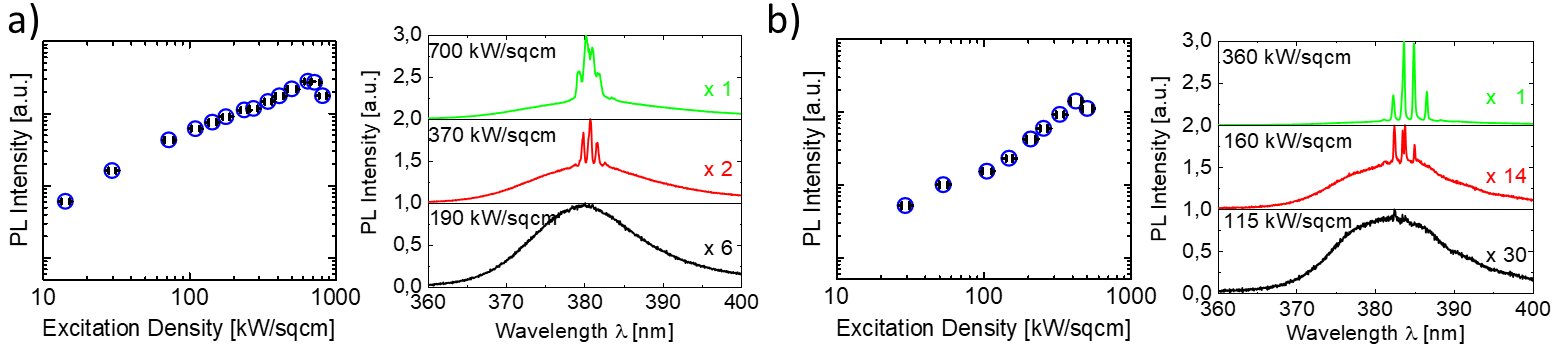
\includegraphics[width=1\textwidth]{Bilder/MgO/CasFit_S1_MgO_1und3}
\caption{Integrierte PL-Intensitäten aufgetragen über der Anregungsdichte, sowie
Spektren bei verschiedenen Anregungsdichten bei einer Spaltbreite von 200
$\upmu$m der beiden Nanodrähte a) ``MgO 1'' und b) ``MgO 2'' aus
\autoref{SEM_MgO_S1_1_3}.} \label{CasFit_S1_MgO_13} \end{figure} Da sich ein
SiO$_\text{2}$-Substrat aufgrund seines diamagnetischen Charakters nicht zum
magnetisieren eignet, wurde im Zuge dieser Masterthesis auch die
Emissionscharakteristik der ZnO-Nanodrähte auf einem
MgO/Co/SiO$_\text{2}$-Substrat untersucht (s. \autoref{MagProb}). Bei den
PL-Messungen mit diesem Substrat fiel auf, dass die Anzahl der Nanodrähte, die
sich überhaupt in den Laserbereich anregen ließen, verglichen mit dem
SiO$_\text{2}$-Substrat, sehr gering war. Auch die Emissionsintensität in den
Moden war deutlich reduziert. Im Folgenden werden zwei Nanodrähte analysiert,
die Moden zeigten (s. \autoref{SEM_MgO_S1_1_3}). Der erste Draht ``MgO 1'' a)
hatte einen Durchmesser von $\text{d} \approx$ 210 nm und eine Länge von
$\text{l} \approx$ 9.8 $\upmu$m, der zweite ``MgO 2'' b) einen Durchmesser von
$\text{d} \approx$ 360 nm und eine Länge von $\text{l} \approx$ 7.3 $\upmu$m. In
\autoref{CasFit_S1_MgO_13} sind die PL-Intensitäten beider Nanodrähte über die
Anregungsdichte aufgetragen. Eine Anpassung nach dem Multimoden-Modell konnte in
beiden Fällen nicht vorgenommen werden, da diese aufgrund der geringen Steigung
im ASE- und Laserbereich nicht konvergierte. Es zeigten sich bei vielen Drähten
Fabry-Pérot-Moden im Bereich um 160 kW/cm$^\text{2}$, entsprechend wäre hier der
ungefähre Laserschwellwert bei 160-190 kW/cm$^\text{2}$ anzusetzen. Dies
entspricht in etwa dem 1.5-fachen bis doppelten des Laserschwellwertes auf
SiO$_\text{2}$. \\ Vergleicht man die Intensitäten der Drähte ``MgO 1 und 2''
aus \autoref{CasFit_S1_MgO_13} mit denen des Drahtes ``SiO$_\text{2}$ 1'' aus
\autoref{SEM_SiO2_S1_6}, zeigen sich große Unterschiede im Laserschwellwert und
in der Intensität höherer Anregungen. Die spontane Emission der NBE ist auch bei
hohen Anregungsdichten in Relation zu den Moden deutlich ausgeprägt. In
\autoref{CasFit_S1_MgO_13} a) zeigt sich im mittleren Spektrum bei 370
kw/cm$^\text{2}$ bis in den deutlich degradierten Bereich bei
700kW/cm$^\text{2}$ keine deutliche Zunahme der Moden. Die Ursache hierfür ist
im geringeren Brechingsindexunterschied zwischen ZnO und MgO, verglichen mit
SiO$_\text{2}$, sowie plasmonischen Verlusten der direkt unterliegenden
Co-Schicht zu finden. Der geringere Brechingsindexunterschied führt zu einem
geringeren Einschlussfaktor des Nanodrahtes gegenüber dem Substrat und somit
dazu, dass die Moden weit in das Substrat eindringen, also evaneszent geführt
werden. In Kombination mit der plasmonisch aktiven Co-Schicht führt dies zu
hohen Verlusten, die nicht nur für das Erreichen des Laserschwellwertes
überbrückt werden müssen, sondern sich auch auf den Anstieg der Laserkurve
auswirken. Es müssen auf diesem Substrat also möglichst dicke Nanodrähte
gefunden werden, um ausreichendes Lasing zu erziehlen, denn für den Draht ``MgO
2'' zeigt sich eine deutliche Verbesserung, wenngleich noch nicht ausreichend
für die Fourieruntersuchungen.\\ \autoref{Spec_MgO} zeigt die Intensitäten der
Drähte ``SiO$_\text{2}$ 1'' aus \autoref{SEM_SiO2_S1_6} und ``MgO 2''
\autoref{CasFit_S1_MgO_13} b) bei verschiedenen Vielfachen des jeweiligen
Laserschwellwertes. Hier fällt auf, dass die Zunahme in der Intensität auf MgO
zwar linear verläuft, aber der Anstieg sehr gering ist. Unterschiede der
Modenabstände hängen maßgeblich mit der Länge der Drähte zusammen, die sich um
einige Mikrometer unterscheiden. Die Moden des Drahtes auf dem
MgO/Co/SiO$_\text{2}$-Substrat sind jedoch gegenüber denen auf dem
SiO$_\text{2}$-Substrat blauverschoben – ein Indiz für eine Hybridmode
\cite{Sidiropoulos.2014}. \\ Der beobachtete Degradationsbereich begann bereits
bei etwa 480kW/cm$^\text{2}$. Beides, der geringe Anstieg und der erhöhte
Laserschwellwert, führte in der Konsequenz dazu, dass für die Fourier-Messungen
dieser Drähte keine ausreichende Statistik zur Verfügung stand.\begin{figure}[b]
\centering 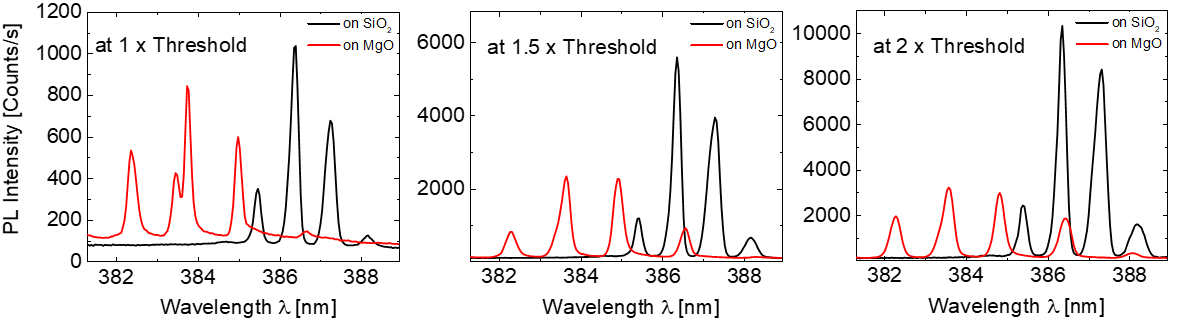
\includegraphics[width=1\textwidth]{Bilder/MgO/Spec_MgO}
\caption{Vergleich der Intensitäten der Drähte aus \autoref{SEM_SiO2_S1_6} und
\autoref{CasFit_S1_MgO_13} b) jeweils ungefähr beim Laserschwellwert, beim
1.5-fachen und 2-fachen Laserschwellwert. Beide Kurven sind jeweils auf die
Belichtungsdauer von einer Sekunde normiert.} \label{Spec_MgO} \end{figure}Über
den Modenabstand der Drähte soll nach \autoref{ResBed}  der Brechungsindex n für
Hochanregung auf dem MgO/Co/SiO$_\text{2}$-Substrat errechnet werden. Hierzu
wurden die Abstände der Moden gemittelt. Es gilt: \begin{equation} n_{Draht 1}
=\frac{\lambda^2}{2L\, \Delta\lambda} + \frac{dn}{d\lambda}\, \lambda= (3.1 \pm
0.6) \text{ ,}\\ n_{Draht 2} =\frac{\lambda^2}{2L\, \Delta\lambda} +
\frac{dn}{d\lambda}\, \lambda= (2.0 \pm 0.5) \text{ ,} \label{RefIndex}
\end{equation} mit den zentralen Wellenlängen $\uplambda_\text{1}=$ 381.2 nm
bzw. $\uplambda_\text{2}=$ 384.7 nm und dem Modenabstand
$\Updelta\uplambda_\text{1}=$ 0.92 nm bzw. $\Updelta\uplambda_\text{2}=$ 1.44 nm
sowie der errechneten Dispersion \autoref{Disp}.\\ Beide Brechungsindizes liegen
weit auseinander und sind mit hohen Fehlern behaftet. Für dünnere Nanodrähte ist
eigentlich anzunehmen, dass der Brechungsindex niedriger liegt als für dickere
Drähte \cite{Zimmler.2010}. Da der Draht ``MgO 1'' jedoch kaum ausgeprägte Moden
zeigte ist anzunehmen, dass die Ladungsträgerdichte deutlich geringer war als im
Draht ``MgO 2''. Entsprechend würde der Brechungsindex zunehmen
\cite{Wille.2016}. Bedenkt man diese Effekte, erscheinen die Brechungsindizes
innerhalb ihrer Fehlertoleranz realistisch, wenngleich der Brechungsindex des
ersten Drahtes wohl am oberen Ende des Fehlers angesiedelt ist. Für
weiterführende Rechnungen im folgenden Abschnitt wird aus diesem Grund der
Brechungsindex für Hochanregung des Drahtes ``MgO 2''  verwendet.
\subsubsection{Drahtkombinationen} Dickere Drähte, die sich später in den
SEM-Messungen als Kombination zweier übereinander liegender Drähte
herausstellten, zeigten eine ausreichende PL-Intensität für die Fouriermessungen
und hatten einen Laserschwellwert ähnlich den Drähten auf SiO$_\text{2}$.
Ansonsten waren sie unter dem Mikroskopaufbau der PL optisch nicht von den
normalen Drähten unterscheidbar. Einer dieser ``kombinierten Drähte'' (s.
\autoref{SEM_MgO_S2_0}), wie sie für die Magnetfeldmessung verwendet wurden,
soll hier ausgewertet werden.\begin{figure}[b] \centering
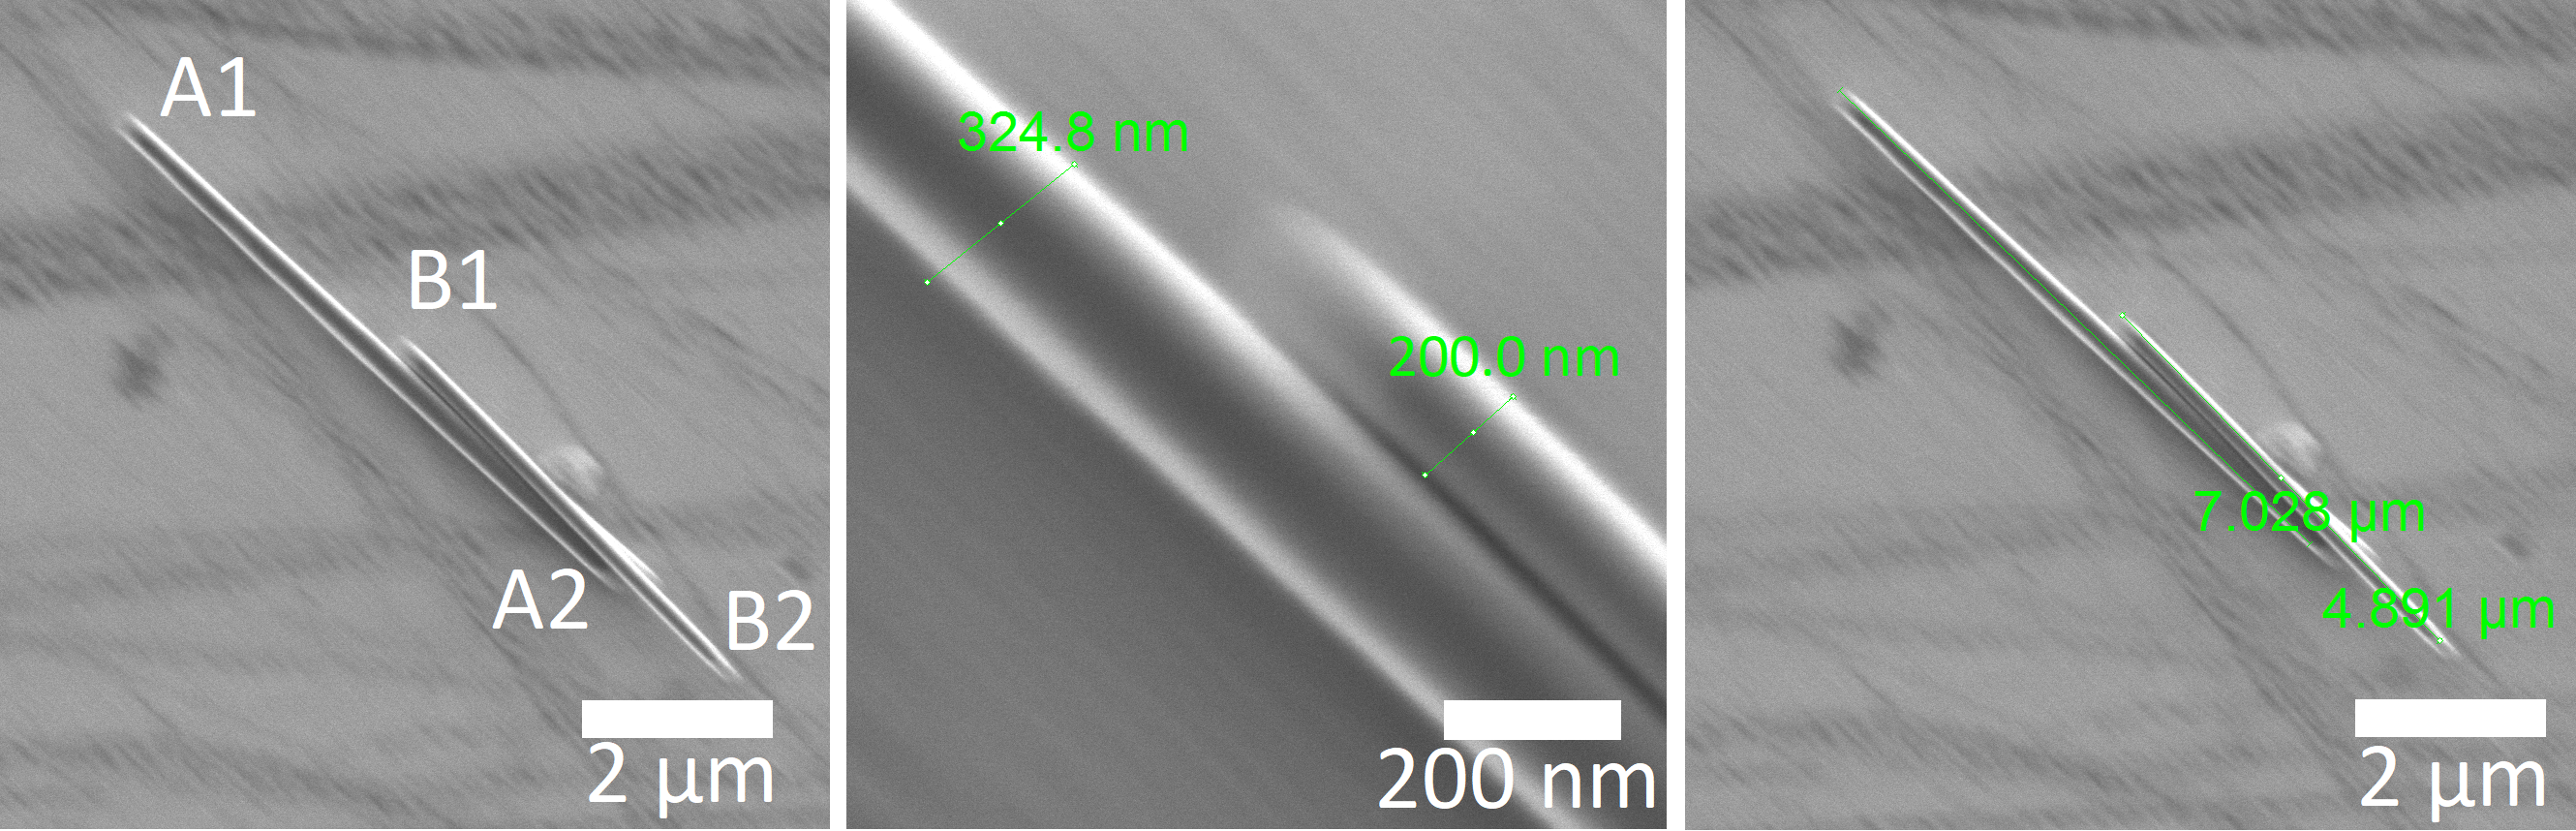
\includegraphics[width=0.7\textwidth]{Bilder/MgO/SEM_MgO_S2_0} \caption{REM-Bild
eines ``kombinierten Nanodrahtes'' mit den Längen \mbox{$\text{l}_\text{A}
\approx \text{7 }\upmu\text{m}$} bzw. \mbox{$\text{l}_\text{B} \approx \text{4.9
} \upmu\text{m}$} und den Durchmessern \mbox{$\text{d}_\text{A} \approx
\text{325 nm}$} bzw. \mbox{$\text{d}_\text{B} \approx \text{200 nm}$}.
Zusammengenommen haben die Drähte eine Gesamtlänge von \mbox{$\text{l} \approx
\text{8.95 } \upmu\text{m}$} und einen Durchmesser von \mbox{$\text{d} \approx
\text{525 nm}$}. Auf dem linken Bild sind zusätzlich die Endfacetten beider
Nanodrähte nummeriert.} \label{SEM_MgO_S2_0} \end{figure} Der untersuchte
``kombinierte Draht'' bestand aus einem etwa 7 $\upmu$m und einem etwa 5
$\upmu$m langen Draht, bei einem Durchmesser von etwa 325 resp. 200 nm. Er
zeigte einen Laserschwellwert bei \mbox{$\approx$ 120 kW/cm$^\text{2}$} und
wurde bei 1.45-fachem Schwellwert untersucht (s. \autoref{Cas_MgO_S2_0}
a)).\begin{figure}[t]
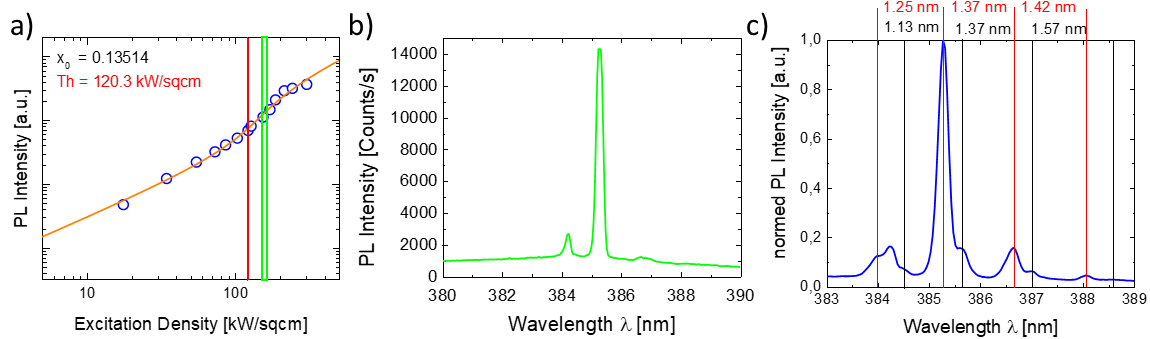
\includegraphics[width=1\textwidth]{Bilder/MgO/Cas_MgO_S2_0} \caption{a)
Integrierte PL-Intensität des kombinierten Nanodrahtes aus
\autoref{SEM_MgO_S2_0} als Funktion der Anregungsleistung. Die durchgezogene
Linie zeigt die Multimoden-Anpassung des Nanodrahtes mit eingezeichneter
Schwellwert-Intensitätsdichte (rot) und Anregungsbereich der Fouriermessungen
(grün). b) Spektrum bei 1.45-fachem Laserschwellwert (155 kW/cm$^\text{2}$) und
Spaltbreite von 200 $\upmu$m. c) Spektrum bei 2.3-fachem Laserschwellwert mit
den schwarzen (der Kaviät L$_\text{1}$) und roten Linien (der Kavität
L$_\text{2}$) sind die Moden einer Kavität gekennzeichnet. Die grün umkreiste
Mode bei $\uplambda=$ 384 nm konnte nicht über Modenabstände zugeordnet werden.
Die dicken Linien kennzeichnen die mittlere Wellenlänge der jeweiligen Kavität.}
\label{Cas_MgO_S2_0} \end{figure}Eine sehr dominante Fabry-Pérot-Mode zeigte
sich bei einer Wellenlänge von \mbox{$\uplambda \approx$ 385.3 nm} \mbox{(s.
\autoref{Cas_MgO_S2_0} b))}, die Moden rechts und links dieser dominanten Mode
treten kaum in Erscheinung. Gleichermaßen ist das Verhältnis der Moden zur NBE
ist gering. Integriert man die Longitudinalmoden in \autoref{Cas_MgO_S2_0} und
vergleicht sie mit der NBE, zeigt sich eine Dominanz der NBE gegenüber den Moden
im Verhältnis von $\approx \text{3:1}$, so wie schon zuvor bei den Einzeldrähten
beobachtet. Dies wird später bei der Polarisation relevant. \\ \begin{table}[h]
\begin{tabular}{llllll} Draht A & Draht B & Facetten A1-B2  & Facetten A1-B1 &
Facetten A2-B1 & Facette A2-B2 \\ 7.03 $\upmu$m & 4.89 $\upmu$m & 8.95 $\upmu$m
& 3.87 $\upmu$m & 3.69 $\upmu$m & 1.56 $\upmu$m \\ \end{tabular}
\caption{Abstände der Endfacetten beider Drähte aus \autoref{SEM_MgO_S2_0}
zueinander, wobei Draht A der dickere unten liegende Draht und Draht B der oben
liegende kurze Draht ist. Die Nummerierung 1 bezieht sich auf die jeweils im
Bild oben liegende Endfacette und entsprechend 2 auf die untere.}
\label{YoungDist} \end{table}Über den Abstand der Moden zueinander kann nach
\autoref{ResBed} die Länge der effektiven Kavität der beiden Drähte berechnet
werden: \begin{equation} L= \frac{\lambda^2}{\Delta \lambda} \,
\left[\frac{1}{2}\,
\left(n(\lambda)-\lambda\cdot\frac{dn(\lambda)}{d\lambda}\right)^{-1}\right]
\text{ .} \end{equation} Da die Brechungsindizes und die Dispersion sowohl von
der geführten Mode, der Wellenlänge und der Dicke des Nanodrahtes abhängen, ist
für eine exakte Berechnung eine FDTD-Simulation notwendig. In diesem Fall soll
eine Näherung des Brechungsindex genügen, die aus der bekannten Längen und den
Modenabständen des Drahtes ``MgO 2'' ermittelt wurde, sowie der Dispersion, die
auf dem SiO$_\text{2}$ errechnet wurde.\\ Bei höheren Anregungsdichten zeigte
sich im Spektrum eine Überlagerung von FP-Moden, die sich eignen die zugehörigen
Kavitäten zu berechnen (s. \autoref{Cas_MgO_S2_0} c)), um herauszufinden welche
Kavitäten effektiv am Laserprozess beteiligt sind und die dominante Mode bilden.
Es ergeben sich damit die Länge der Kavitäten: \begin{equation} &L_1= (8.2 \pm
1.1)\, \mu m\text{ ,}\\ &L_2= (7.7 \pm 1.1)\, \mu m\text{ ,}\ \end{equation} mit
den zentralen Wellenlänge $\uplambda_\text{1}=\text{386.2}$ nm bzw.
$\uplambda_\text{2}=\text{386.5}$ nm und den mittleren Modenabständen
$\Updelta\uplambda_\text{1}=\text{1.28}$ nm bzw.
$\uplambda_\text{2}=\text{1.36}$ nm sowie der berechneten Dispersion aus
\autoref{Disp} und dem Brechungsindex  von Draht 2 (s. \autoref{RefIndex}). Es
konnten zwei Modenprofile verschiedener Kavitäten analysiert werden. Diese
passen innerhalb ihrer Fehler ausschließlich zum Draht A, sowie zur kombinierten
Kavität der Drähte A und B, wobei die kombinierte Kavität wahrscheinlich die
dominante Mode bei $\uplambda=$ 385.3 nm stellt. Eine weitere Mode bei
$\uplambda=$ 384.0 nm konnte aufgrund fehlender weiteren Moden nicht zugeordnet
werden, es erscheint aber sinnvoll, diese dem kleineren Nanodraht B zuzuordnen.
Mit 200 nm Durchmesser ist dieser Draht ziemlich dünn, es deutet also darauf
hin, dass ein Teil der Moden des kleinen Drahtes B in dem anderen Draht A
geführt und dort weiter verstärkt werden. Dies deckt sich mit der Beobachtung,
dass die Emission primär an äußeren Endfacetten austrat, eine mittige Emission
war nicht zu beobachten und wurde wahrscheinlich überstrahlt.
\subsection{Fourierabbildung der Nanodrahtemission} Betrachtet man das
Fourierbild in nullter Beugungsordnung (s. \autoref{S0_S2_MgO_0} a), so zeigt
sich auch hier ein deutliches Interferenzmuster, das moduliert ist. Im Gegensatz
zu \autoref{S0_S1_Si02_6} ist das Interferenzmuster hier gerade und nicht am
Rand gebogen. Gleichzeitig zeigt sich in erster Beugungsordnung (s.
\autoref{S0_S2_MgO_0} b), dass die Mode bei $\uplambda = $ 385.3 nm die größte
Emissionsdichte aufweist. \begin{figure}[h] \centering
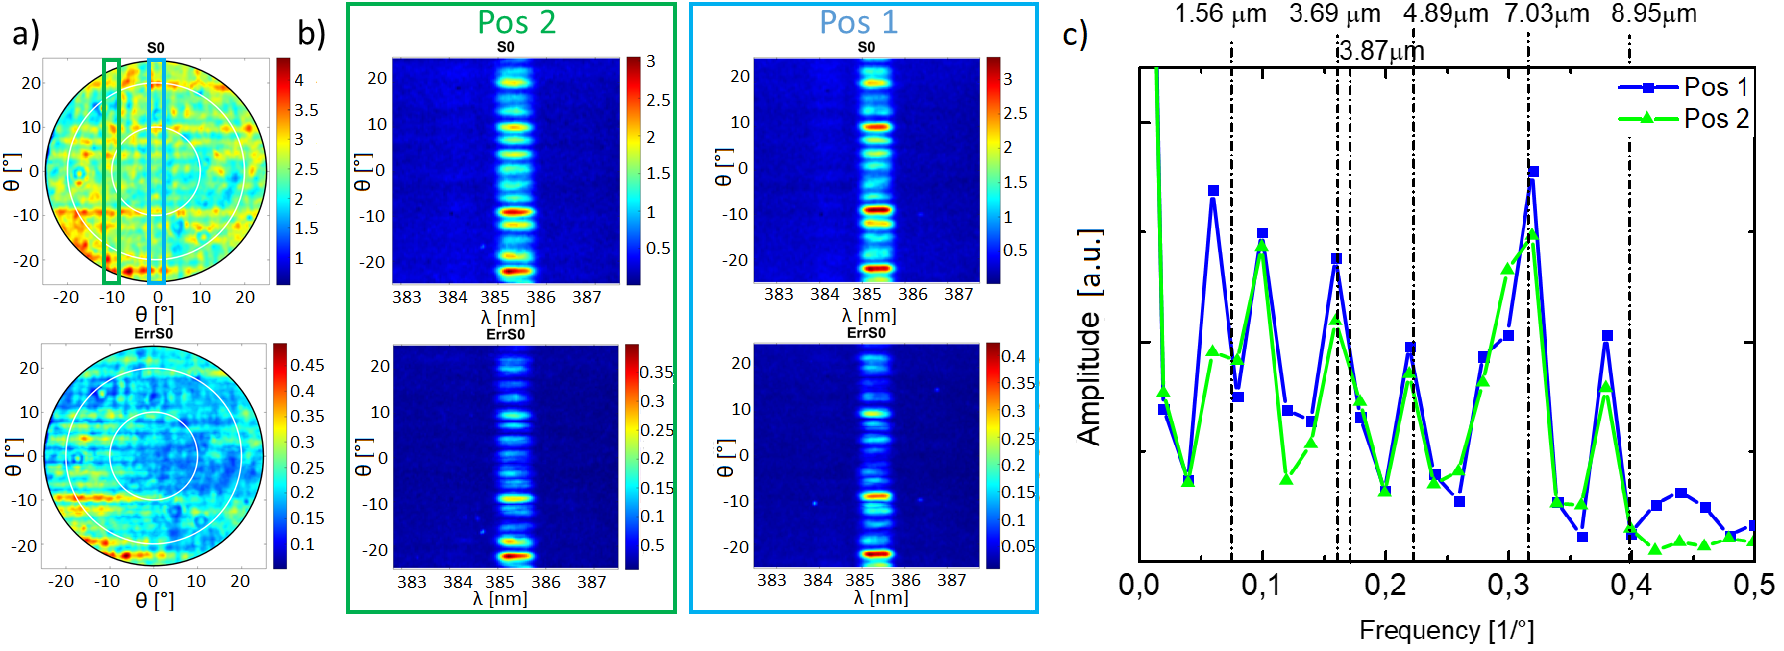
\includegraphics[width=1\textwidth]{Bilder/MgO/S0_S2_MgO_0} \caption{Obere
Reihe: Darstellung der rekonstruierten Gesamtintensitäten des Drahtes aus
\autoref{SEM_SiO2_S1_6} nach Stokes in a) nullter Beugungsordnung mit der blauen
Markierung von Position 1 und der grünen von Position 2 sowie b) in erster
Beugungsordnung an Position 1 und 2 bei 1.3-fachem Laserschwellwert. Untere
Reihe: Die jeweiligen absoluten Fehler und c) Fourieranalyse von Profilen des
Interferenzmusters der Mode bei $\uplambda=$ 385.3 nm aus b) an den Positionen 1
und 2. Gestrichelt dargestellt sind Frequenzen, die die Abstände der Endfacetten
beider Nanodrähte zu den jeweils anderen Endfacetten repräsentieren würden.}
\label{S0_S2_MgO_0} \end{figure}Eine Fourieranalyse des Interferenzmusters aus
erster Beugungsordnung ist in \autoref{S0_S2_MgO_0} c) dargestellt. Über die
REM-Aufnahme lassen sich die verschiedenen Abstände der Endfacetten zueinander
ermitteln (s. \autoref{YoungDist}) und über Umstellen der \autoref{Distance} zu
\begin{equation} f=\frac{1}{arctan\left(\frac{\lambda}{d}\right)} \end{equation}
in Frequenzen eines Interferenzmusters überführen. Diese Frequenzen sind als
gestrichelte Linie mit den jeweiligen Abständen der Facetten in selbiger
Abbildung dargestellt. Es zeigt sich im Frequenzspektrum eine gute
Übereinstimmung für eine Überlagerung von Interferenzmustern der Endfacetten von
Draht A  und der Endfacetten von Draht B sowie der Interferenz der beiden
Endfacetten von Draht A mit der oberen Endfacette von Draht B. Die beiden
restlichen Frequenzen sind gegenüber dem Erwartungswert verschoben, jedoch
innerhalb der Messauflösung. Insgesamt passt das Interferenzmuster zu der
kombinierten Kavität mit ihren vier Endfacetten.\\ Der große Draht A wirkt in
diesem Fall also eher als haupttreibender Prozess und wirkt gleichermaßen als
Abstandhalter für den kleinen Draht zum dämpfenden Substrat. Dieser kleine Draht
B kann somit, trotz seiner geringen Dicke, als zusätzliches Verstärkermedium
dienen und den Laserprozess weiter verstärken. Hierbei formt sich eine
zusätzliche gemeinsame Kavität, die Drähte koppeln.
\subsection{Polarisationseigenschaften der Nanodrahtemission} In
\autoref{DOP_MgO_S2_0} sind die Polarisationsgrade a) in nullter und b) in
erster Beugungsordnung dargestellt. In nullter Beugungsordnung zeichnet sich
deutlich das Interferenzmuster ab.\begin{figure}[b] \centering
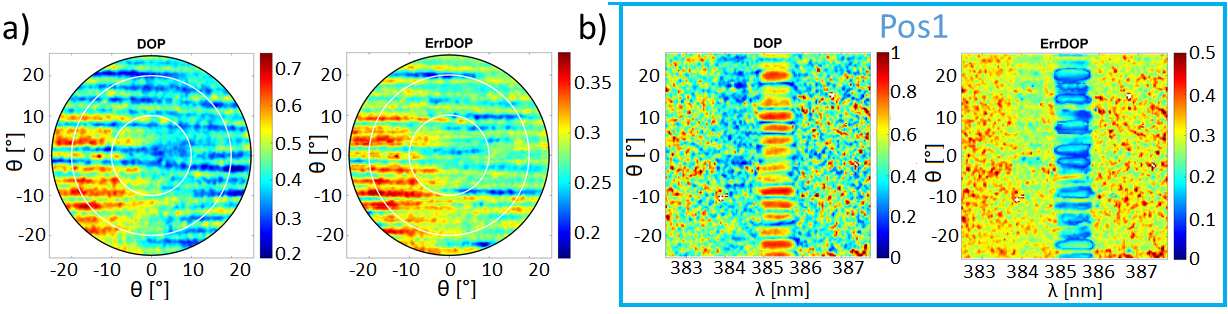
\includegraphics[width=1\textwidth]{Bilder/MgO/DOP_MgO_S2_0} \caption{Links:
Darstellung des DOP in a) nullter Beugungsordnung und b) in erster
Beugungsordnung an Position 1 bei 1.3-fachem Laserschwellwert. Rechts: Die
jeweiligen absoluten Fehler.} \label{DOP_MgO_S2_0}
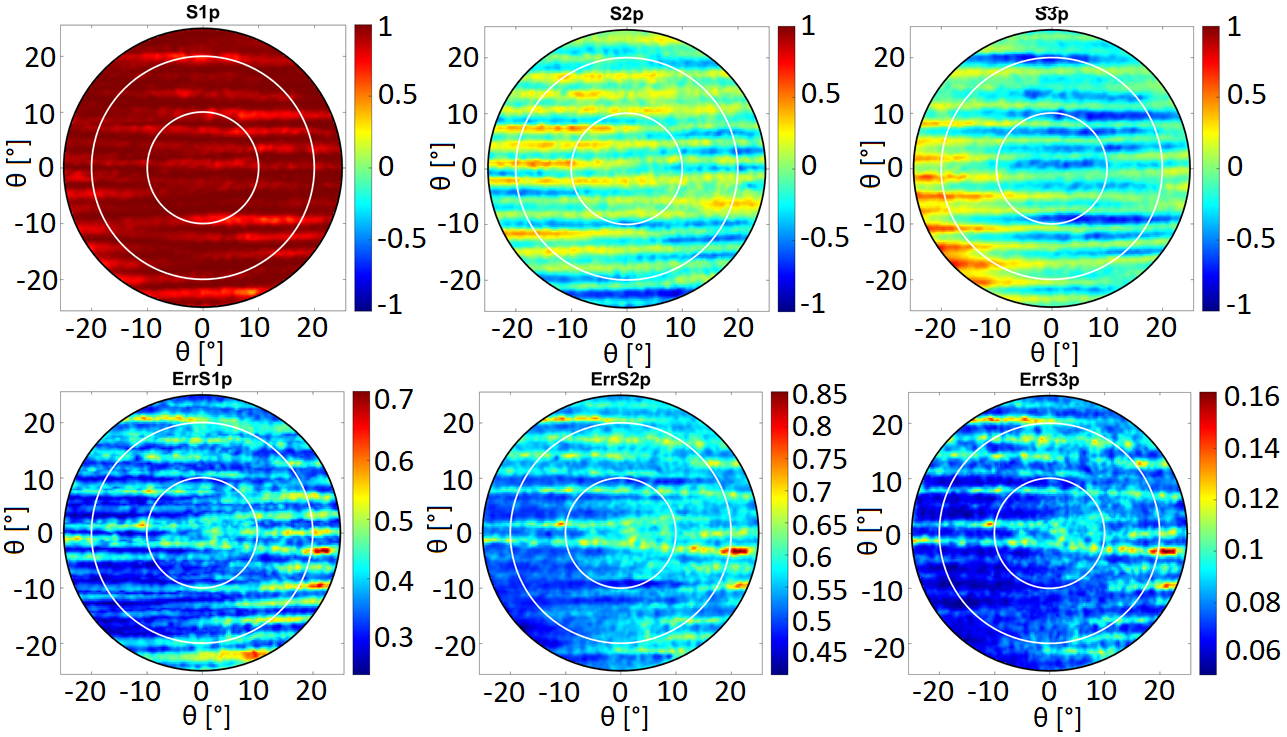
\includegraphics[width=0.75\textwidth]{Bilder/MgO/StokesP_S2_MgO_0}
\caption{Obere Reihe: Darstellung der auf den polarisierten Anteil der Emission
normierten Stokes-Parameter des Nanodrahtes aus \autoref{SEM_MgO_S2_0} in
nullter Beugungsordnung. Zur besseren Vergleichbarkeit sind die Stokes-Parameter
gleich skaliert. Untere Reihe: Die jeweiligen absoluten Fehler.}
\label{StokesP_S2_MgO_0} \end{figure}Hierbei fällt auf, dass der Kontrast höher
ist als auf SiO$_\text{2}$ in \autoref{DOP_SiO2_S1_6} a), da sich hier nur eine
FP-Mode ausprägt. \autoref{DOP_MgO_S2_0} b) zeigt, dass die Longitudinalmode zu
hohem Anteil polarisiert ist. Gleichzeitig zeigt sich, dass auch auf dem
MgO/Co/SiO$_\text{2}$-Substrat die NBE polarisiert ist. Dies wird vor allem beim
Vergleich der Stokes-Parameter in nullter wie erster Beugungsordnung (s.
\autoref{StokesP_S2_MgO_0} und \autoref{SpecP1_StokesP_S2_MgO_0}) wichtig. Somit
zeigen beide Beugungsordnungen zeigen völlig unterschiedliche Trends. Während in
nullter Beugungsordnung eindeutig der S$_\text{1,p}$-Parameter dominiert und auf
eine horizontale Polarisation hindeutet, zeigt sich in erster Beugungsordnung,
dass die FP-Mode eher Anteile vertikal polarisierten Lichtes führt, während die
NBE weiter horizontal polarisiert bleibt. Dies könnte auf Anteile einer TM-Mode
hindeuten, die auf einem plasmonischen Substrat auch zu erwarten wäre.
Multipliziert man den Gesamtanteil der NBE  und den der Moden an der Emission
mit ihren Polarisationen, ergeben sich entprechende Verteilungen der
Stokes-Parameter wie in \autoref{StokesP_S2_MgO_0} beobachtet. Wenn dies auch
zunächst dem ersten Eindruck widerspricht, zeigt sich doch bei genauerer Analyse
eine gute Übereinstimmung und verdeutlicht die Notwendigkeit der spektralen
Aufspaltung.\\ In den spektral aufgelösten Stokes-Parametern sticht vor allem
der S$_\text{3,p}$-Parameter heraus. Dies verdeutlicht vor allem ein Profil der
Moden, dargestellt in \autoref{SpecP1_StokesP_Line_S2_MgO_0} a). Es zeigt sich,
dass an den gestrichelt dargestellten Positionen der Maxima des
Interferenzmusters der S$_\text{3,p}$-Parameter $\approx$ -1 ist und somit die
Mode eindeutig linkszirkular polarisiert ist. Ursächlich hierfür könnte die
Vermischung der Transversalmoden beider Drähte sein. Mit dem Versatz des oben
liegenden Drahtes könnten die Nahfelder durch eine Phasenverschiebung zueinander
in Rotation geraten und somit zirkular polarisiertes Licht entstehen lassen (s.
\autoref{SpecP1_StokesP_Line_S2_MgO_0} b). Diese Vermutung wird auch von der
gemeinsam wirksamen Kavität unterstützt, lässt sich jedoch im Rahmen dieser
Masterthesis nicht abschließend klären und bedarf weiterer Experimente und
Simulationen. \begin{figure}[h] \centering
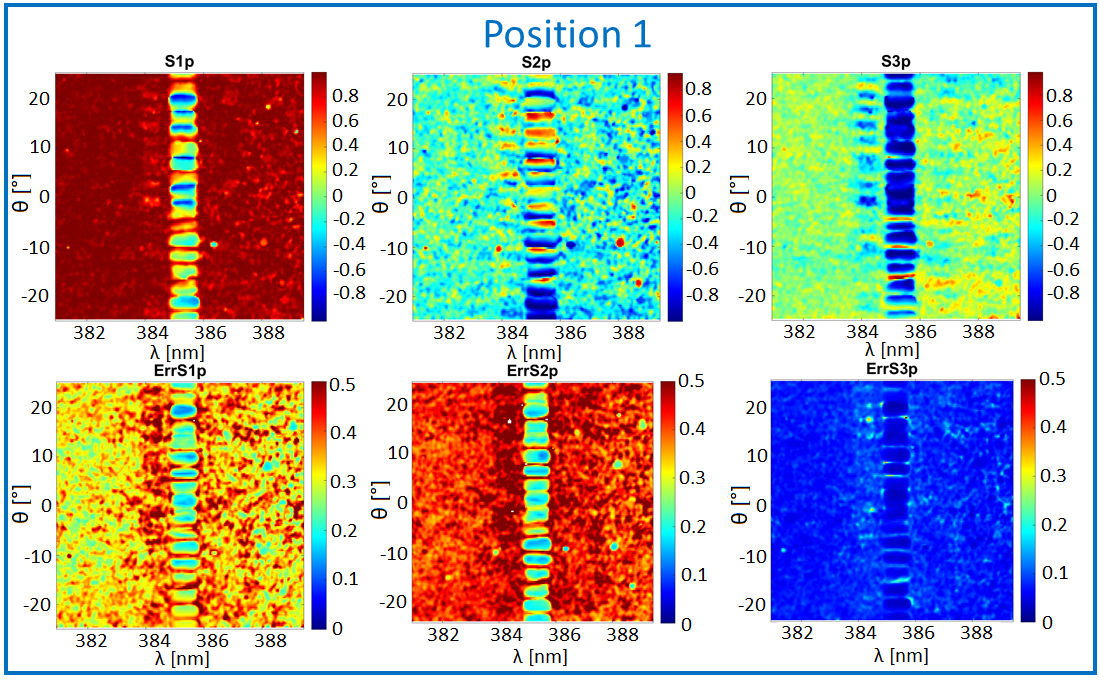
\includegraphics[width=0.8\textwidth]{Bilder/MgO/SpecP1_StokesP_S2_MgO_0}
\caption{Obere Reihe: Darstellung der spektral aufgelösten und auf den
polarisierten Anteil der Emission normierten Stokes-Parameter des Nanodrahtes
aus \autoref{SEM_MgO_S2_0} an Position 1. Zur besseren Vergleichbarkeit sind die
Stokes-Parameter gleich skaliert. Untere Reihe: Die jeweiligen absoluten
Fehler.} \label{SpecP1_StokesP_S2_MgO_0}
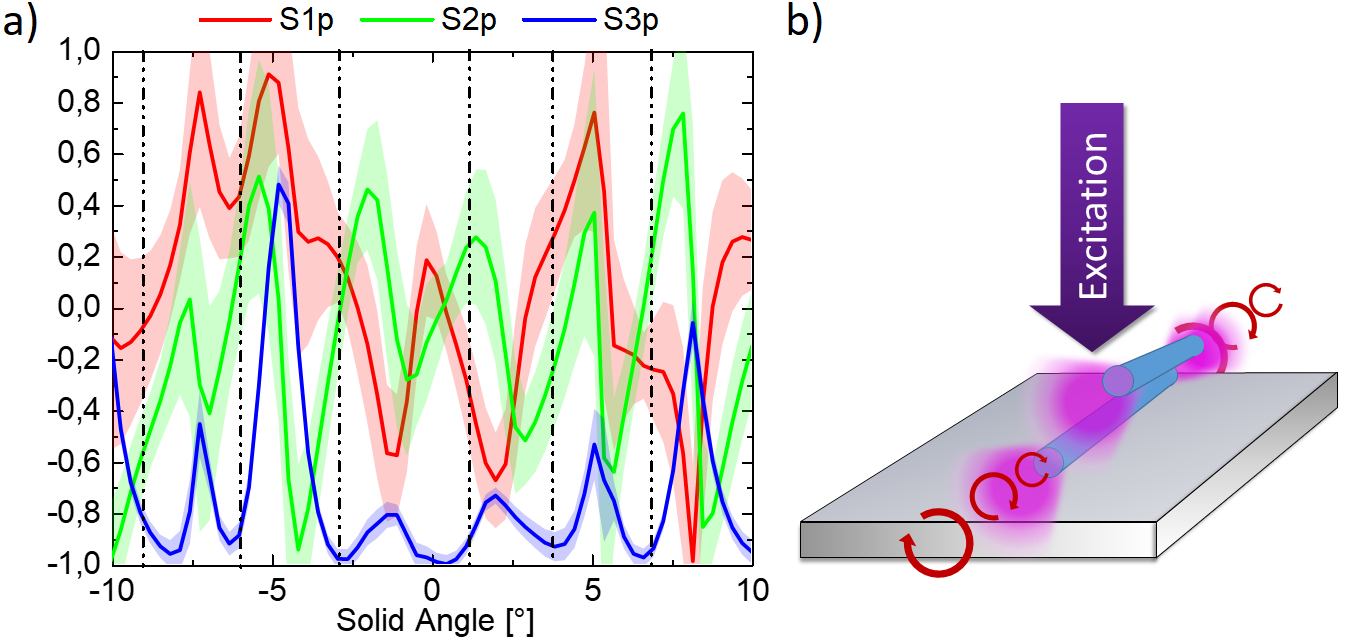
\includegraphics[width=.6\textwidth]{Bilder/MgO/SpecP1_StokesP_Line_S2_MgO_0}
\caption{a) Profile der Stokes-Parameter aus \autoref{SpecP1_StokesP_S2_MgO_0}
der dominanten Mode bei \mbox{$\uplambda=$ 385.3 nm}. Schwarz gestrichelt
dargestellt sind die Positionen der Interferenzmaxima der Gesamtintensität aus
\autoref{S0_S2_MgO_0} b) an Position 1. b) Schematische Darstellung der
linkszirkularen Polarisation der Laseremission des kombinierten Nanodrahtes auf
einem MgO/Co/SiO$_\text{2}$-Substrat.} \label{SpecP1_StokesP_Line_S2_MgO_0}
\end{figure} \chapter{Einfluss eines externen Magnetfeldes auf die
Emissionscharakteristik} In diesem Kapitel soll der Einfluss eines externen
Magnetfeldes auf die Emission von Nanodrähten untersucht werden. Hierzu wurden
Nanostrukturen auf ein magnetisier- bares MgO/Co/SiO$_\text{2}$-Substrat
aufgebracht und zwei davon (s. \autoref{SEM_Mag} a) und b)) zunächst ohne
Magnetfeld untersucht. Danach wurde das Substrat mithilfe der Helmholtzspule (s.
\autoref{Sim}) in orthogonaler bzw. paralleler Ausrichtung zur Nanodrahtachse
$\vec{\textbf{c}}$ magnetisiert. Um das Substrat in die Sättigungsmagnetisierung
zu bringen, wurde die Spule für wenige Sekunden in Betrieb genommen und vor der
PL-Messung wieder ausgeschaltet.\\ \begin{figure} \centering
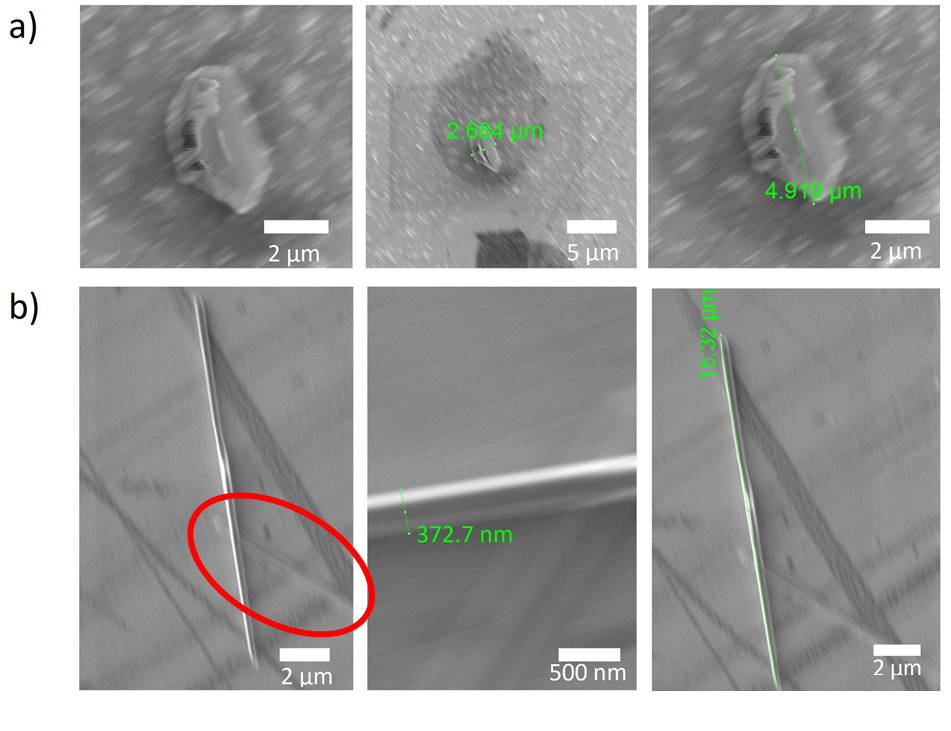
\includegraphics[width=.66\textwidth]{Bilder/Mag/SEM_Mag1} \caption{REM-Bilder
der Nanodrähte a) ``Mag 1'' mit einem Durchmesser von d $\approx$ 2.7 $\upmu$m
und der Länge l $\approx$ 4.9 $\upmu$m sowie b) ``Mag 2'' mit einem Durchmesser
von d $\approx$ \mbox{360.6 nm} und der Länge l $\approx$ 15.3 $\upmu$m. Dabei
wird dieser Nanodraht im Bereich des roten Kreises von einem weiteren Nanodraht
überlagert, der hier defokussiert erscheint.} \label{SEM_Mag} \end{figure} Es
sollen hierdurch auftretende Unterschiede im Spektrum und im Laserschwellwert
diskutiert werden, um danach auf die Stokes-Parameter einzugehen. Hierbei wurden
die Stokes-Parameter der Emission spektral und winkelaufgelöst untersucht, um
NBE und die FP-Moden separiert betrachten zu können. Es wurden dabei die
Erkenntnisse des vorherigen Kapitels berücksichtigt. In der Fehlerbetrachtung
der Stokes-Messungen werden hier sämtliche systematischen Fehler ausgeblendet,
da sie die vergleichenden Messungen in selber Weise verfälschen, aber keine
gesonderten Unterschiede erzeugen. Die Fehler dieser Messungen sind hier
folglich deutlich reduziert.\\ Interessant erscheint ein deutliches
Laserverhalten des Drahtes ``Mag 1'' (s. \autoref{SEM_Mag} a)), der im REM-Bild
eigentlich wenig Ähnlichkeiten mit einem Draht aufwies, aber trotzdem bei
Anregung eine Endfacettenemission und Moden- wie Laserverhalten zeigte. Jedoch
zeigt eine einfache Rechnung nach \autoref{ResBed}, dass der Modenabstand für
Fabry-Pérot-Moden nicht zu der Kavitätslänge passt: \begin{equation} L=(8.2 \pm
1.1)\, \mu m \text{ ,} \end{equation} mit der zentralen Wellenlänge $\uplambda =
\text{386.06 nm}$, dem mittleren Modenabstand $\Updelta \uplambda = \text{1.27
nm}$, den ermittelten Werten für den Brechungsindex n $=$ 2 sowie der Dispersion
$\frac{\text{dn}}{\text{d}\uplambda} = \text{13.26} \upmu\text{m}$, verglichen
mit der gemessenen Länge von l $=$ 4.9 $\upmu$m. Da jedoch kein weiterer
Nanodraht in der Nähe von ``Mag 1'' lag, muss davon ausgegangen werden, dass es
sich um diesen Draht handelt. Der Grund für den zu kleinen Modenabstand konnte
nicht geklärt werden, denn der Modenabstand passt auch nicht für
\textit{Whispering-Gallery-Moden}. \section{Spektrum und Laserschwellwert} In
\autoref{Spectr_Mag} sind die Messungen der beiden Nanodrähte ``Mag 1'' (oben)
und ``Mag 2'' (unten) zusammengefasst. Dabei befindet sich in Spalte a) die
komplette Laserkurve des jeweiligen Drahtes mit einer
Multimoden-Anpassung.\begin{figure}[b] \centering
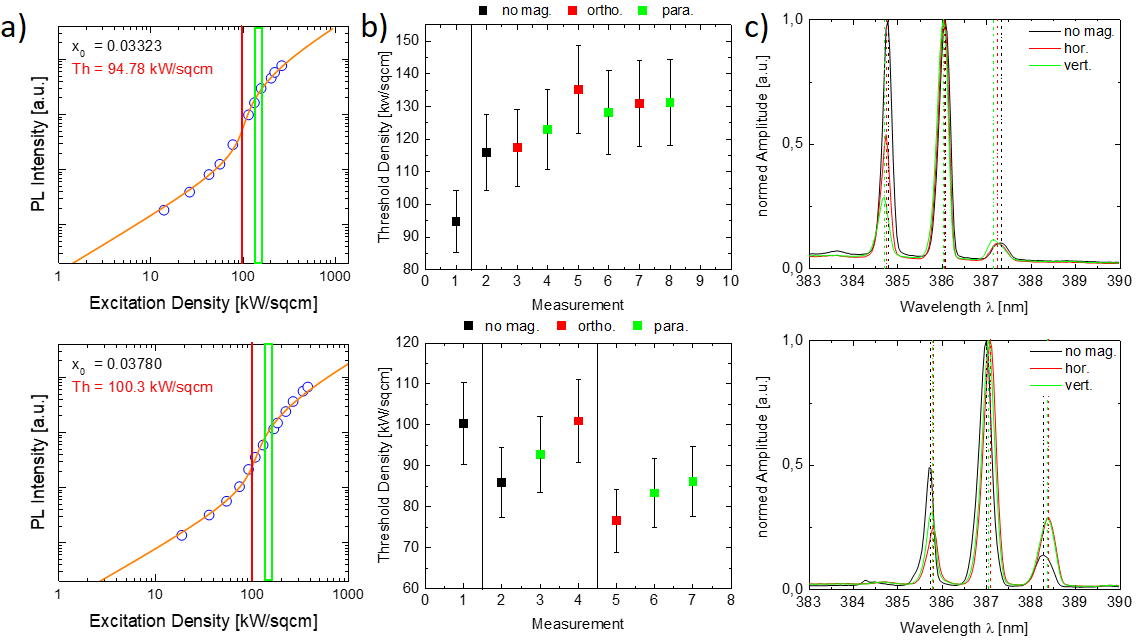
\includegraphics[width=1\textwidth]{Bilder/Mag/Spectr_Mag} \caption{Obere Reihe:
Messungen des Nanodrahtes ``Mag 1''. Untere Reihe: Messungen des Nanodrahtes
``Mag 2''. \textbf{Spalte a)} Integrierte PL-Intensität der Nanodrähte aus
\autoref{SEM_Mag} als Funktion der Anregungsleistung ohne externes Magnetfeld.
Die durchgezogene Linie zeigt die Multimoden-Anpassung des Nanodrahtes mit
eingezeichneter Schwellwert-Intensitätsdichte (rot) und Anregungsbereich der
Fouriermessungen (grün). \mbox{\textbf{Spalte b)}} Laserschwellwert des
jeweiligen Nanodrahtes ohne sowie mit orthogonaler bzw. paralleler
Substratmagnetisierung. Mit schwarzen Linien sind Neuausrichtungen des
jeweiligen Nanodrahtes im Laserspot gekennzeichnet. \textbf{Spalte c)} Spektren
bei ca. 150 kW/cm$^\text{2}$ und Spaltbreite von 200 $\upmu$m für die Messungen
ohne, sowie mit horizontalem und vertikalem Magnetfeld. Die Spektren sind
jeweils auf ihr Maximum normiert. Gestrichelt dargestellt sind die jeweiligen
Maxima der FP-Moden.} \label{Spectr_Mag} \end{figure} Der so ermittelte
Laserschwellwert wird im ersten Bereich der Graphen in Spalte b) (abgegrenzt
durch die erste schwarze Linie) dargestellt. Die Graphen b) zeigen die
Schwellwertdichte des jeweiligen Nanodrahtes ohne und mit orthogonal bzw.
parallel zur Nanodrahtachse angelegtem externen Magnetfeld. Zwischen den
einzelnen Schwellwertmessungen wurden spektral aufgelöste Fouriermessung der
Stokes-Parameter bzw. Stokes-Messungen des Spektrums vorgenommen. Während dieser
Messungen zeigte sich, dass sich die Probe relativ zum Anregungslaser verschob.
Dies wird auch im Ansteigen des Laserschwellwerts mit zunehmender Anzahl
Messungen sichtbar. Dass dieser Anstieg nicht von Degradationsprozessen
herrührt, zeigt ein Absinken des Laserschwellwerts auf den ungefähren
Ursprungswert nach einer Neujustierung (in \autoref{Spectr_Mag} b) unten). Die
Nanodrähte rückten also aus der optimalen Position im Laserspot heraus und
mussten neu positioniert werden, diese Neujustierungen wurden mit schwarzen
vertikalen Linien in den Graphen gekennzeichnet. Innerhalb der Messauflösung
kann nicht bestimmt werden, ob und wie sich der Laserschwellwert durch das
Anlegen der Magnetfelder verändert hat. In Spalte c) sind die Spektren bei ca.
150 kW/cm$^{2}$ dargestellt. Da sich der Laserschwellwert während der Messungen
verändert hat, wurden alle drei Spektren bei unterschiedlichen vielfachen ihres
Laserschwellwerts gemessen. Durch eine Normierung auf das Maximum des jeweiligen
Spektrums zeigen also die anderen Moden unterschiedliche Höhen. Mit
gestrichelten Linien wurden die jeweiligen Maxima der FP-Moden gekennzeichnet.
Beim Anlegen eines externen Magnetfeldes sieht man einen leichten Versatz der
Modenmaxima zueinander. Dieser Versatz liegt aber an der Auflösungsgrenze des
Spektrometers. Weiterhin zeigt der Versatz im Vergleich der Drähte (Reihenfolge
oben: grün, rot, schwarz; Reihenfolge unten: schwarz, grün, rot) beim Anlegen
der verschiedenen Felder keine konsistente Reihenfolge. Diese Verschiebungen
resultieren großteils aus den dynamischen Inhomogenitäten in der Pumpleistung
und -verteilung des Anregungslasers und zeigten sich auch bei Mehrfachmessungen
einer Anregungsdichte ohne Anlegen eines Magnetfeldes. Ein Vergleich der
Intensitäten und der Intensitätsverhältnisse der Moden zueinander war,
wenngleich interessant, leider nicht möglich, da sich die Nanodrähte
zwangsläufig verschoben und sich somit Laserschwellwert und Anregungsprofil
veränderten. Dies führt durch Inhomogenitäten des Laserspots in der Konsequenz
dazu, dass sich die Intensitätsverhältnisse der Moden zwangsweise verändern
mussten – eine Vergleichbarkeit war nicht mehr gegeben. \\ Die Auswertung der
Spektren und des Laserschwellwertes gibt also keine signifikant nachweisbaren
Änderungen  im Lasingverhalten der Nanodrähte durch externe Magnetfelder preis
und ist durch die kurzen Belichtungszeiten und großen Schwankungen innerhalb der
Spektren stark fehlerbelastet. Diese Methode eignet sich also nicht, um im
gewählten Versuchsaufbau effektive Änderungen durch das Anlegen eines
Magnetfeldes nachzuweisen. \section{Polarisationsgrad und Stokes-Parameter} Da
weder Spektrum noch Laserschwellwert hinreichende Änderungen zeigten, sollen nun
die Polarisationseigenschaften der Emission untersucht werden.\begin{figure}[b]
\centering \includegraphics[width=0.8\textwidth]{Bilder/Mag/DOP_Spec_Mag}
\caption{Fourierbilder der DOP des Nanodrahtes ``Mag 1'' (\autoref{SEM_Mag} a))
in erster Beugungsordnung bei 1.3-fachem Laserschwellwert (ca. 150
kW/cm$^\text{2}$) ohne (schwarz) sowie mit orthogonal (rot) und parallel (grün)
ausgerichtetem externen Magnetfeld.} \label{DOP_Spec_Mag} \end{figure} Für den
Draht ``Mag 1'' (aus \autoref{SEM_Mag} a)) sind die Polarisationsgrade für die
drei Magnetfeldmessungen bei ca. 1.3-fachen Laserschwellwert in
\autoref{DOP_Spec_Mag} dargestellt. Um eine bessere Übersicht über die
Polarisationsgrade verschiedener Substratmagnetisierungen zu erlangen, sind
diese als Profil über die vertikalen Raumwinkel in \autoref{DOP_Mag}
dargestellt. Dabei zeigt sich, dass der Polarisationsgrad innerhalb der FP-Moden
innerhalb der Fehlertoleranzen konstant bleibt (s. \autoref{DOP_Mag} Oben: a)).
Für den Nanodraht ``Mag 2'' bei ca. 1.8-fachem Laserschwellwert ergibt sich ein
ähnliches Bild (s. \autoref{DOP_Mag} b) erste Spalte), wobei hier die
Polarisationsgrade innerhalb der Mode nicht signifikant zunehmen. Auch ein
erneuter Vergleich der Polarisationsgrade bei orthogonalem bzw. parallelem
externen Magnetfeld zeigt, dass es zwischen beiden Magnetfeldausrichtungen keine
signifikante Änderung des Polarisationsgrades in der Mode gibt (s.
\autoref{DOP_Mag} b) zweite Spalte).\\\begin{figure}[b] \centering
\includegraphics[width=1\textwidth]{Bilder/Mag/DOP_Mag} \caption{a) Profile über
den Polarisationsgrad der Moden und der NBE der Drähte a) \mbox{``Mag 1''} und
b) ``Mag 2''. Obere Reihe: Profil des Polarisationsgrades der FP-Mode bei a)
$\uplambda_\text{1}=$386 nm bei 1.3-fachem Laserschwellwert bzw. b)
$\uplambda_\text{1}=$ 387 nm bei 1.8-fachem Laserschwellwert, jeweils ohne
externes Magnetfeld (schwarz) sowie bei orthogonal (rot) und parallel (grün)
ausgerichteten Magnetfeldern. Die vertikalen schwarzen Linien markieren die
jeweiligen Maxima des Interferenzmusters der FP-Mode. Untere Reihe: Gemittelter
Polarisationsgrad der NBE bei gleichen Laserschwellwerten und bei
\mbox{$\uplambda=$ 379.5 - 382.5 nm}. Die horizontalen Linien zeigen den
Mittelwert des Polarisationsgrades über die vertikalen Raumwinkel. Bei b) sind
in der zweiten Spalte zusätzlich zwei weitere Messungen der Polarisationsgrade
bei horizontalem und vertikalem externen Magnetfeld dargestellt.}
\label{DOP_Mag} \end{figure} Im Gegensatz hierzu verändert sich bei
unterschiedlichen Magnetfeldern der Polarisationsgrad der NBE stark (s.
\autoref{DOP_Mag} Unten: a) und b)). Hierbei fällt auf, dass sich der
Polarisationsgrad durch das Anlegen eines parallelen Magnetfeldes signifikant
erhöhen lässt. Gleichzeitig sieht es so aus, als würde das Anlegen eines
orthogonalen Magnetfeldes den Polarisationsgrad der NBE senken. Deutlich
erkennen lässt sich jedoch, dass ein paralleles Magnetfeld deutlich höhere
Polarisationsgrade erzeugt als ein orthogonales (s \autoref{DOP_Mag} b) zweite
Spalte unten).\\ Ähnlich wie mit dem Polarisationsgrad verhält es sich auch mit
den Stokes-Parametern. In \autoref{Stokes_Spec_Mag} ist exemplarisch der
S$_\text{3,p}$-Parameter in erster Beugungsordnung abgebildet. Gerade der
S$_\text{3,p}$-Parameter ist interessant, da bei ihm eine Abhängigkeit vom
Magnetfeld zu erwarten wäre. Durch das Vorhandensein eines externen Magnetfeldes
kommt es zur Zeeman-Aufspaltung, die eine gewisse Spinpolarisation bewirkt und
der Spinvektor der Ladungen in eine Larmorpräzession gerät (s. \autoref{Zee}) –
es wird also ein externer Drehimpuls eingebracht, der eine zirkulare
Polarisation der Emission bewirken könnte.\begin{figure}[h] \centering
\includegraphics[width=.85\textwidth]{Bilder/Mag/Stokes_Spec_Mag}
\caption{Fourierbild des S$_\text{3,p}$-Parameters des Nanodrahtes ``Mag 1''
(\autoref{SEM_Mag} a)) in erster Beugungsordnung bei 1.3-fachem Laserschwellwert
(ca. 150 kW/cm$^\text{2}$) ohne (schwarz) sowie mit orthogonal (rot) und
parallel (grün) ausgerichtetem externen Magnetfeld.} \label{Stokes_Spec_Mag}
\centering \end{figure} In \autoref{Stokes_Mag} sind, zur besseren
Vergleichbarkeit, Profile der Stokes-Parameter über die vertikalen Raumwinkel
dargestellt. Es zeigt sich auch hier, dass sich innerhalb der FP-Mode nichts
signifikant ändert. Für beide Drähte bleibt die horizontale Polarisation
(sichtbar im S$_\text{1,p}$ in \autoref{Stokes_Mag}) deutlich dominant, kleine
Abweichungen liegen allesamt innerhalb der Fehlertoleranzen. Ähnlich wie bereits
in \autoref{PolGradSiO2} beschrieben, steigen die anderen Stokes-Parameter nur
zwischen den FP-Modenmaxima. \autoref{Stokes_NBE_Mag} stellt Profile der
gemittelten Stokes-Parameter über die vertikalen Raumwinkel für die NBE dar und
zeigt, dass sich für beide Nanodrähte die Stokes-Parameter stark verändern,
\autoref{Stokes_NBE_repeat}, eine Wiederholungsmessung nach einer
Repositionierung des Nanodrahtes im Laserspot unter zweimaligem
Magnetfeldwechsel spricht dagegen.\begin{figure}[h]
\includegraphics[width=1\textwidth]{Bilder/Mag/Stokes_Mag} \caption{Profile der
normierten Stokes-Parameter in erster Beugungsordnung der Moden a) des Drahtes
``Mag 1''  bei $\uplambda=$ 386 nm bei 1.3-fachem Laserschwellwert und b) des
Drahtes ``Mag 2'' bei $\uplambda=$ 387 nm und 1.8-fachem Laserschwellwert. Beide
Drähte wurden bei verschiedenen Magnetfeldern gemessen, jeweils ohne externes
Magnetfeld (schwarz) sowie bei orthogonal (rot) und parallel (grün)
ausgerichteten Magnetfeldern. Die vertikalen schwarzen Linien zeigen die
jeweiligen Maxima der FP-Moden.} \label{Stokes_Mag} \centering
\includegraphics[width=1\textwidth]{Bilder/Mag/Stokes_NBE_Mag}
\caption{Gemittelte Stokes-Parameter der NBE bei bei \mbox{$\uplambda=$ 379.5 -
382.5 nm} der Drähte a) ``Mag 1'' bei 1.3-fachen Laserschwellwert und b) ``Mag
2'' bei 1.8-fachem Laserschwellwert. Beide Drähte wurden bei verschiedenen
Magnetfeldern gemessen, jeweils ohne externes Magnetfeld (schwarz) sowie bei
orthogonal (rot) und parallel (grün) ausgerichteten Magnetfeldern. Die
horizontalen Linien zeigen den Mittelwert der Stokes-Parameter über die
vertikalen Raumwinkel.} \label{Stokes_NBE_Mag} \end{figure}  Letztendlich geht
aus dem Messungen nicht klar und schlüssig hervor, ob und wenn ja inwiefern sich
die Stokes-Parameter verändern. Um hier eine eindeutige Aussage zu treffen,
wären konsistente Messergebnisse nötig.\\ Es lässt sich also aussagen, dass sich
weder die Polarisation noch die Stokes-Parameter innerhalb der Fabry-Pérot-Moden
ändern. Da diese Emission aus einem Laserprozess resultiert, muss der
Polarisationsgrad DOP $\approx$ 1 sein, und zwar unabhängig von jeweiligen
externen Feldern. Dass sich die Stokes-Parameter innerhalb der Fabry-Pérot-Moden
nicht verändern, liegt an den unterschiedlichen Einschlussfaktoren der
verschiedenen Transversalmoden (s. \autoref{abhd}). Dies führt zur einer
Selektion der stabilsten Transversalmode, die wiederum für die
Polarisationsrichtung bestimmend ist. Dieser Selektionsparameter ist bedeutend
wichtiger für das Ausbilden der Transversalmode als etwaige geringe
Energieverschiebungen unter den verschiedenen Exzitonen aufgrund der
Zeeman-Aufspaltung (s. \autoref{Zee}). Auch die Position der Fabry-Pérot-Moden
im Spektrum muss dieselbe bleiben (s. \autoref{FPModen}), da diese
Longitudinalmoden die Resonanzbedingung der Kavität erfüllen müssen. Andere
spektrale Positionen sind instabil. Somit sind die Energie der Photonen
innerhalb der Longitudinalmoden, der Polarisationsgrad und die
Polarisationsrichtung vordefiniert, unabhängig vom Magnetfeld. Im Falle mehrerer
anschwingender Transversalmoden, also einer Vermischung, könnte sich ein anderes
Verhältnis einstellen, dies konnte hier aber nicht beobachtet werden. Hierzu
wären Messungen in der ``Head-On''-Geometrie, einer Sichtposition direkt in eine
Endfacette des Nanodrahtes, nötig, die im Rahmen dieser Masterthesis nicht
vorgenommen wurden.\\ Die NBE, im Gegensatz zur Tranversalmode der
Laseremission, ist an keinen Einschlussfaktor gebunden. Hier spielen alleinig
die verschiedenen Bandübergänge eine Rolle, die durch Zeeman-Aufspaltung
verändert werden. Das Anlegen eines Magnetfeldes parallel zur Nanodrahtachse
führt zu einer verstärkten Emission horizontal polarisierter Photonen auf Kosten
der vertikal polarisierten. Durch den D'yakonov-Perel'-Mechanismus (s.
\autoref{DPM}) kommt es durch das angelegte Magnetfeld zu einer Erhöhung der
Spinrelaxationszeit der Exzitonen – ein Spinflip wird unwahrscheinlicher (s.
\autoref{DPM_Mag}).\FloatBarrier \noindent Dies führt dazu, dass die geringen
Übergangswahrscheinlichkeiten der X$_\text{A}$- und X$_\text{B}$- Exzitonen für
vertikal polarisiertes Licht (s. \autoref{spinueb}) weiter sinken, da der
Spinflip unterdrückt wird. Eine gleichmäßige Mischung aus horizontal und
vertikal polarisiertem Licht erscheint nach dem Formalismus der Stokes-Parameter
als unpolarisiertes Licht. Da das Magnetfeld nun dafür sorgt, dass mehr
horizontal polarisiertes Licht entsteht, folgt eine Entmischung, die sich als
Steigen des Polarisationsgrades bemerkbar macht. Für ein orthogonal anliegendes
Magnetfeld gilt dies aufgrund des Hanle-Effekts, der den Effekt des Magnetfeldes
umkehrt, nicht (s. \autoref{Hanle}). Entsprechend ist für ein orthogonales
Magnetfeld eine Absenkung des Polarisationsgrades gegenüber dem unmagnetisierten
Zustands zu erwarten. Für eine Bestätigung letzterer These bedarf es aber
weiterer Messungen, die Messdaten liefern hier lediglich Anhaltspunkte. Selbiges
gilt für die Stokes-Parameter der NBE. Hier kann aufgrund widersprüchlicher
Messdaten keine konkrete Aussage getroffen werden. Aufgrund des extern
zugeführten Drehimpulses wäre zumindest theoretisch eine Erhöhung des
S$_\text{3,p}$-Parameters erwartbar gewesen. Die NBE zeigt insgesamt ein großes
Rauschen, das eine Auswertung schwierig und fehleranfällig macht, sodass die
hier erzielten Ergebnisse mit Vorsicht zu betrachten sind. \begin{figure}[h]
\centering \includegraphics[width=1\textwidth]{Bilder/Mag/Stokes_NBE_repeat}
\caption{Wiederholte Messungen der gemittelte Stokes-Parameter der NBE
(\mbox{$\uplambda=$ 379.5 - 382.5 nm}) der Drahtes ``Mag 2'' bei 1.8-fachem
Laserschwellwert und orthogonal (rot) bzw. parallel (grün) ausgerichteten
Magnetfeldern.} \label{Stokes_NBE_repeat} \end{figure} \chapter{Zusammenfassung
und Ausblick} In dieser Masterthesis wurde die Emissionscharakteristik von
ZnO-Nanodrähten auf SiO$_\text{2}$- und MgO/Co/SiO$_\text{2}$-Substraten
winkelaufgelöst in nullter und erster Beugungsordnung des Monochromators
untersucht. Hierzu wurden die Nanodrähte aus der ``Top-View''-Geometrie
betrachtet und das entstehende Interferenzmuster untersucht. Hierzu wurde ein
Fourieraufbau in den $\upmu$-PL Aufbau integriert und die Stokes-Parameter
mithilfe der Methode der rotierenden $\uplambda$/4-Platte bestimmt. Zur
Auswertung wurde das Matlabskript von Max Riediger \cite{Riediger.Master}
erweitert und an die hiesige Messungen angepasst. Zudem wurde eine umfangreiche
Fehlerrechnung implementiert.\\ Wie erwartet zeigte sich, dass es sich bei dem
Interferenzmuster um die Interferenz nach Young handelt, nach der sich die
beiden Endfacetten des Nanodrahtes wie die Öffnungen im Doppelspaltexperiment
verhalten. Es konnte in erster Beugungsordnung, also spektral aufgelöst, gezeigt
werden, dass die Interferenzmaxima benachbarter Fabry-Pérot-Moden aufgrund der
Resonanzbedingung um $\uppi$ phasenverschoben sind. Da die so phasenverschobenen
Fabry-Pérot-Moden ineinander fallen, sinkt der Kontrast des Interferenzmusters
stark. Der Kontrast konnte jedoch in erster Beugungsordnung, durch spektrale
Trennung der Moden, deutlich erhöht werden.\\ Auch zeigte sich, dass die
Intensitätsverhältnisse der Moden zueinander innerhalb der Messauflösung
konstant bleiben und dies überall innerhalb der maximal in diesem Versuchsaufbau
auflösbaren Raumwinkel von ca $\pm \text{25}^\circ$. Gleichzeitig konnte gezeigt
werden, dass die Emission innerhalb der Moden fast vollständig polarisiert und
auch die Polarisation außerhalb der Moden in der NBE mit ca. 50-60\% nicht
vernachlässigbar ist. Dies resultiert aus der Bandstruktur von ZnO, die
bevorzugt eine Emission horizontal polarisierten Lichtes nahe der Bandkante
emittiert. Dieses Resultat unterstützt die Messergebnisse von Jacopin et al.
(2011) \cite{Jacopin.2011}. Ferner zeigte sich für die beiden untersuchten
Substrate eine horizontale Polarisation der NBE.\\ ZnO-Nanodrähte auf einem
SiO$_\text{2}$-Substrat zeigen eine horizontale Polarisation innerhalb der
Fabry-Pérot-Moden, dies deutet auf eine TE-Transversalmode hin und passt somit
zu den FDTD-Simulationen betreffender Nanodrahtdicke (s. \autoref{abhd}). Zudem
sind der Polarisationsgrad und die Stokes-Parameter aller longitudinalen
Fabry-Pérot-Moden gleich, sodass davon ausgegangen werden kann, dass alle
Fabry-Pérot-Moden in derselben Transversalmode oder derselben Überlagerung
verschiedener Transversalmoden schwingen. Sie entspringen also den selben
Nahfeldern. Um dies zweifelsfrei zu verifizieren, bedarf es aber weiterer
FDTD-Simulationen und Messungen.\\ Für das MgO/Co/SiO$_\text{2}$-Substrat zeigte
sich, verglichen zum SiO$_\text{2}$-Substrat, ein erhöhter Laserschwellwert bei
ähnlichen Nanodrahtdurchmessern, gleichzeitig ein flacher Anstieg der Intensität
im Lasingbereich, sodass auf diesem Substrat ausschließlich besonders dicke oder
sich überlagernde Nanodrähte eine ausreichende Emissionsintensität zeigten, um
die Fouriermessungen sinnvoll mit ihnen betreiben zu können.\\ Einer dieser
``kombinierten'' Drähte wurde analysiert und zeigte ein überlagertes
Modenspektrum. Mithilfe von Kalkulationen der Modenabstände über die
Resonanzbedingung konnten zwei Kavitäten separiert werden, von denen die
emissionstärkste der kombinierten Kavität beider Drähte entsprach. Hierzu wurde
die Dispersion von ZnO-Nanodrähten bei Hochanregung und der Brechungsindex der
Nanodrähte auf dem MgO/Co/SiO$_\text{2}$-Substrat berechnet – beide Werte lagen
innerhalb ihrer Fehlertoleranz im Bereich des Erwartbaren. Auch das
Interferenzmuster in erster Beugungsordnung zeigte eine Modulation, die sich als
Überlagerung der Young'schen Interferenzen der verschiedenen Endfacetten
herausstellte.\\ Diese Ergebnisse legen nahe, dass beide Drähte koppeln. Eine
linkszirkulare Polarisation der Mode konnte nachgewiesen werden und wurde darauf
zurückgeführt, dass die Nahfelder beider Drähte phasenverschoben in
unterschiedlichen Transversalmoden schwingen, woraus sich rotierende Felder
ergeben würden, die in der Konsequenz zu zirkular polarisiertem Licht führen
würden. Zu einer Bestätigung dieser Hypothese bedürfte es allerdings
weiterführender Simulationen und weiterer Experimente zur Bestätigung.\\
Weiterhin wurde die Emission bei angelegten externen Magnetfeldern untersucht.
Hierzu wurde eine Helmholtzspule  simuliert, dimensioniert und in den
Versuchsaufbau implementiert. Die Feldlinien der Spule konnten \textit{in situ}
um 90$^\circ$ parallel und orthogonal zur Nanodrahtachse ausgerichtet werden.
Für diese Messungen wurden die ZnO-Nanodrähte auf das magnetisierbare
MgO/Co/SiO$_\text{2}$-Substrat aufgetragen, um höhere lokale Feldstärken zu
generieren. Durch den ``Proximity-Effekt'' sollte eine Spinpolarisation erzeugt
werden und deren Einfluss auf die Emission untersucht werden.\\ Hierzu wurden
zwei Nanodrähte untersucht, die beide eine ausreichende Emissionsintensität
zeigten. In der Auswertung der Spektren und der Laserschwellwerte ergab sich
keine signifikante Änderung innerhalb der Messauflösung. Die Position der
Fabry-Pérot-Moden im Spektrum ist aufgrund der Resonanzbedingung fixiert. Es
zeigte sich in den Laserschwellwerten aber, dass sich die Drähte im Laufe der
Messungen ohne weiteres Zutun verschoben. Die Ursache hierfür konnte nicht
abschließend geklärt werden. Es wird aber vermutet, dass dies durch das
notwendige wiederholte Eingreifen in den Versuchsaufbau zum Messen der
Stokes-Parameter verursacht wurde. Gleichzeitig könnte auch das Schalten des
Magnetfeldes zu einer Verschiebung geführt haben. Dieses Verschieben machte es
notwendig, den Nanodraht immer wieder neu zu positionieren und mag in gewissem
Umfang zu Veränderungen in der Emission geführt haben. Insgesamt traten solche
Veränderungen durch eine Repositionierung in den Hintergrund und führten
lediglich zu einer Senkung des Laserschwellwertes auf das vorherige Niveau.\\ Es
zeigte sich in den winkelaufgelösten Messungen in erster Beugungsordnung, dass
die Emission innerhalb der longitudinalen Fabry-Pérot-Moden konstant blieb.
Innerhalb der Fehlertoleranz konnte beim Anlegen des Magnetfeldes und beim
Wechsel der Magnetisierungsrichtung keine signifikante Veränderung festgestellt
werden, da hier der Einschlussfaktor der bestimmende Faktor für die
Transversalmode ist, der Einfluss des Magnetfeldes scheint zu gering, um eine
Veränderung herbeizuführen.\\ Für die NBE zeigte sich jedoch eine signifikante
und reproduzierbare Erhöhung des Polarisationsgrades für die Ausrichtung der
Spule parallel zur Nanodrahtachse, die auf den D'yakonov-Perel'-Mechanismus
zurückgeführt wurde. Für die orthogonale Ausrichtung des Magnetfeldes zeigen die
Messdaten zumindest eine Tendenz zur Depolarisierung, die aufgrund des
Hanle-Effekts erwartbar wäre. Eine Veränderung der Stokes-Parameter innerhalb
der NBE konnte, aufgrund widersprüchlicher Messdaten, nicht gezeigt werden.\\\\
Insgesamt zeigt diese Masterthesis Ergebnisse, die weiterführender Messungen
bedürfen. Hierzu wäre es sinnvoll ein Objektiv mit höherer numerischer Apertur
NA zu verwenden, um aus dem Interferenzmuster in nullter Beugungsordnung
Informationen über die Longitudinalmode zu erlangen \cite{Saxena.2015}. Dies
würde zwar die Auflösung der Raumwinkel verringern, aber auch mehr Licht
auffangen. So würde sich die Statistik bei gleicher Anregung deutlich verbessern
und damit das Rauschen der normierten Stokes-Parameter vor allem in erster
Beugungsordnung deutlich reduzieren.\\ Interessant wäre, die Kopplung zweier
Nanodrähte genauer zu betrachten, da sich die Laserintensität dadurch deutlich
erhöhen ließe. Durch die Kopplung der Felder beider Drähte wäre es denkbar, über
einen Versatz beider Drähte und einer Verkippung beider Nanodrahtachsen, die
Stokes-Parameter der Emission zu steuern. Hierzu müsste aber eine genaue
Platzierung der Nanodrähte vorgenommen werden. Weiterhin wäre es interessant,
die Polarisation der NBE unter veränderlichen externen Magnetfeldern genauer zu
untersuchen. Hier könnte beispielsweise auf den dauerstrich Helium-Cadmium
(HeCd)-Laser  der $\upmu$-PL zurückgegriffen werden. Dieser erzeugt nicht die
nötige Besetzungsinversion und es bilden sich keine Lasermoden im Nanodraht aus.
Somit wird primär NBE abgestrahlt, die unter viel besserer Statistik untersucht
werden könnte. Gleichzeitig könnte untersucht werden, ob sich die
Wellenleitereigenschaften hierdurch verändern. Dies wäre im Bereich des
denkbaren, vor allem in Bezug auf die plasmonische Kopplung an das Substrat.\\
Um zu untersuchen, ob sich im Falle mehrerer anschwingender Transversalmoden das
Intensitätsverhältnis dieser Moden untereinander unter externen Magnetfeldern
verändert, wären Messungen in der ``Head-On''-Messgeometrie vorzunehmen. Zudem
hätte eine solche Messung entweder mit dickeren Nanodrähten oder einer
Veränderung des Substrates zu erfolgen, um die Nanodrähte in den Laserbereich
anzuregen.\\ In dieser Masterthesis konnte gezeigt werden, dass nur ein
Laserbetrieb von sehr dicken Nanodrähten auf dem MgO/Co/SiO$_\text{2}$-Substrat
möglich ist. Der Ansatz, statt MgO SiO$_\text{2}$ als oberste Schicht zu
verwenden, hat den Vorteil eines höheren Brechungsindexunterschiedes zwischen
Nanodraht und Substrat und könnte dazu beitragen, die Verluste durch das
Substrat einzudämmen. Weiterhin kann überlegt werden, die obere Schicht dicker
zu wählen, hierbei muss jedoch Rücksicht auf die Reichweite des
``Proximity-Effektes'' zur spontanen Spinkohärenz berücksichtigt werden.\\
Anhand spezifischer Merkmale der Transversalmoden lassen sie sich voneinander
unterscheiden \cite{Roeder.Diss}. In der Überlagerung mehrerer Transversalmoden
müssten sich also die Intensitätsverhältnisse der einzelnen Transversalmoden
zueinander verändern. Dies wäre ein klares Indiz für eine magnetfeldinduzierte
Veränderung der Lasereigenschaften, die in dieser Masterthesis nicht gezeigt
werden konnte. Diese Messungen sollten mit weiterführenden FDTD-Simulationen
einhergehen, um die Ergebnisse besser einordnen zu können.
